\documentclass[degree=master,tocarialchapter]{thuthesis}
% 选项
%   degree=[bachelor|master|doctor|postdoctor], % 必选,学位类型
%   language=[chinese|english], % 可选(默认:chinese),论文的主要语言
%   secret,                % 可选(默认:关闭),是否有密级
%   tocarialchapter,       % 可选(默认:关闭),章目录中使用黑体(这项表示同时打开下面两项)
%   tocarialchapterentry,  % 可选(默认:关闭),单独控制章标题在目录中使用黑体
%   tocarialchapterpage,   % 可选(默认:关闭),单独控制章页码在目录中使用黑体

% 所有其它可能用到的包都统一放到这里了,可以根据自己的实际添加或者删除。
\usepackage{thuthesis}
\usepackage{algorithm}
\usepackage{algorithmicx}
\usepackage{algpseudocode}
\usepackage{subfigure}
\usepackage{graphicx}

% 定义所有的图片文件在 figures 子目录下
\graphicspath{{figures/}}
% 可以在这里修改配置文件中的定义。导言区可以使用中文。
% \def\myname{薛瑞尼}

\begin{document}

%%% 封面部分
\frontmatter
\thusetup{
  %******************************
  % 注意:
  %   1. 配置里面不要出现空行
  %   2. 不需要的配置信息可以删除
  %******************************
  %
  %=====
  % 秘级
  %=====
  secretlevel={秘密},
  secretyear={10},
  %
  %=========
  % 中文信息
  %=========
  ctitle={气候系统模式集合预测的关键技术研究},
  %v\version
  cdegree={工学硕士},
  cdepartment={计算机科学与技术系},
  cmajor={计算机科学与技术},
  cauthor={吴利},
  csupervisor={薛巍副教授},
  %cassosupervisor={陈文光教授}, % 副指导老师
  %ccosupervisor={某某某教授}, % 联合指导老师
  % 日期自动使用当前时间,若需指定按如下方式修改:
  % cdate={超新星纪元},
  %
  % 博士后专有部分
  catalognumber     = {分类号},  % 可以留空
  udc               = {UDC},  % 可以留空
  id                = {编号},  % 可以留空: id={},
  cfirstdiscipline  = {计算机科学与技术},  % 流动站(一级学科)名称
  cseconddiscipline = {系统结构},  % 专 业(二级学科)名称
  postdoctordate    = {2009 年 7 月——2011 年 7 月},  % 工作完成日期
  postdocstartdate  = {2009 年 7 月 1 日},  % 研究工作起始时间
  postdocenddate    = {2011 年 7 月 1 日},  % 研究工作期满时间
  %
  %=========
  % 英文信息
  %=========
  etitle={Key Technology Research on Ensemble Prediction of Climate System Model},
  %v\version
  % 这块比较复杂,需要分情况讨论:
  % 1. 学术型硕士
  %    edegree:必须为Master of Arts或Master of Science(注意大小写)
  %             “哲学、文学、历史学、法学、教育学、艺术学门类,公共管理学科
  %              填写Master of Arts,其它填写Master of Science”
  %    emajor:“获得一级学科授权的学科填写一级学科名称,其它填写二级学科名称”
  % 2. 专业型硕士
  %    edegree:“填写专业学位英文名称全称”
  %    emajor:“工程硕士填写工程领域,其它专业学位不填写此项”
  % 3. 学术型博士
  %    edegree:Doctor of Philosophy(注意大小写)
  %    emajor:“获得一级学科授权的学科填写一级学科名称,其它填写二级学科名称”
  % 4. 专业型博士
  %    edegree:“填写专业学位英文名称全称”
  %    emajor:不填写此项
  edegree={Master of Engineering},
  emajor={Computer Science and Technology},
  eauthor={Wu Li},
  esupervisor={Professor Xue Wei},
  %eassosupervisor={Chen Wenguang},
  % 日期自动生成,若需指定按如下方式修改:
  % edate={December, 2005}
  %
  % 关键词用“英文逗号”分割
  ckeywords={集合预测;不确定性量化;代理模式;机器学习;气候系统模式},
  ekeywords={ensemble prediction, uncertainty quantification, surrogate model, machine learning,climate system model}
}

% 定义中英文摘要和关键字
\begin{cabstract}
%气候系统模式集合预测是提升预报能力的重要方法。然而由于物理过程参数和初值的不确定性等原因导致气候预测存在严峻的挑战。降低气候集合预测中的物理参数和初值不确定性对提升预测能力至关重要。
%本文提出了一种基于参数优化的气候系统模式初值集合方法(BGMOPT)。此方法首先对气候系统模式中的不确定性参数进行优化,然后将优化参数后的模式用于初值集合预测。

物理方案参数不确定性量化是减小参数不确定性,提升气候系统模式模拟水平的重要方法,但是当前常用的进化算法等在复杂的气候系统模式上的应用需要极高的时间和计算成本,急需快速高效的参数优化方法。针对此现状,本文提出了一组基于多层感知机神经网络的代理模式参数优化方法,有力支持单目标优化、多目标优化和有约束优化多种模式参数估计场景。本文提出的优化算法与当前常用的优化算法在复杂数学函数和单柱大气模式上的评测结果表明,新提出的算法在精度和收敛性上具有总体优势。在复杂单柱大气模式上,本文的多目标优化方法收敛速度可相对NSGAIII方法提升5倍以上。

初值集合扰动方法对降低初值不确定性,意义重大。然而当前气候预测中常用的滞后平均法(LAF)缺乏较强的理论基础。本文提出了一种面向气候预测的增长模繁殖法(BGM),此方法是在天气预测BGM的基础上结合了气候预测特征对初始繁殖扰动生成,繁殖循环长度选取等关键技术进行了重构,重构后的方法更能适应气候预测中增长最快扰动的获取。为了进一步验证方法的有效性,BGM方法与国家气候中心当前使用的LAF方法在BCC-CSM气候系统模式上进行了15年的对比回报试验,试验结果表明新提出的BGM方法在第一个月的预测结果中相比LAF方法改进明显,500hpa(百帕)位势高度的均方根误差相对于LAF方法预测结果减小了10\%。部分变量的改进效果可延伸至四个月。

融合上述技术,本文设计了一种面向气候预测的集合方法(BGMOPT)并实现了相应的气候预测系统原型,针对国家气候中心的BCC-CSM模式,以热带大气季节内振荡(MJO)和东亚夏季风(EASM)为目标,以辐射平衡为约束对不确定性参数进行优化,将优化后的参数用于BGM初值扰动集合,结果表明BGMOPT方法在2008年12月到2009年3月的气候预测案例中表现良好。四个月全球降水与观测的均方误差相比原LAF方法改进15\%。进一步,本文提出了一种基于机器学习的集合预测集成方法以针对重要的预报指标生成最优的确定性预报结果,此方法结合了观测和模式输出数据的特征,对BCC-CSM模式输出的集合预测结果进行修正与集成,此方法在厄尔尼诺/南方涛动(ENSO)的预测中,海表温度与观测的均方根误差可相对于传统的集合平均法改进32\%.

%另外由于2008年12月为中国几十年难得一见的寒潮现象。本文分析了在中国北方的降水和地表温度等指标,新的方法相比原方法分别改进**倍和**倍。
%此类优化算法与进化算法中以种群为单位更新优化策略的方法不同,而是每一个最新样本都需要调整优化策略,因此提高了收敛速度。而相对于基于插值模型的传统代理模式,此类方法的代理回归精度更高,从而提升了优化策略的决策能力,提升了算法的准确率。
\end{cabstract}

% 如果习惯关键字跟在摘要文字后面,可以用直接命令来设置,如下:
% \ckeywords{\TeX, \LaTeX, CJK, 模板, 论文}

\begin{eabstract}
Parameter uncertainty quantification approaches are used to reduce parameter uncertainty and improve the simulation skill of climate system model. However, the application of current popular evolutionary algorithms in complex climate system models requires long time and high computational cost. For cost expensive climate system models, fast and effective parameter optimization methods need to be further studied. This paper proposes a set of parameter optimization methods based on multilayer perceptron surrogate model targeting single objective optimization, multi-objective optimization and constrained optimization. The evaluation results of the proposed optimization algorithms and the commonly used optimization algorithms with complex mathematical functions and single-column atmospheric modes show that the proposed algorithms have overall advantages in accuracy and convergence. With the complex single column atmospheric model, the convergence rate of the proposed multi-objective optimization method can be improved by more than 5 times compared with the known NSGAIII method.

The initial condition perturbation method of ensemble is of great significance for the study of reducing the initial uncertainty. However, the currently used Lagged Average Forecasting(LAF) method lacks a strong theoretical foundation. This paper proposes a Breeding of Growing Mode(BGM) method for climate prediction, based on the BGM method for weather prediction. And the key techniques in BGM method, such as initial perturbation generation and breeding cycle length, are reconstructed. The reconstructed method is more adaptable to obtain the fastest growing perturbation in climate prediction. This paper compares the proposed BGM method with the LAF method currently used by the National Climate Center in the BCC-CSM climate system model. 15-years hindicast results show that the BGM method is significantly better than the LAF method in the prediction of most climate variables in the first month. The 500hpa potential height is improved by 10\% relative to the LAF method in term of RMSE(root mean square error). The improvement effect of some variables can be extended to four months.

Finally, this paper designs a new climate ensemble method (BGMOPT) for climate prediction, by integration of the proposed parameter optimization method and the BGM, which is compared with the LAF method in the BCC-CSM model. With BCC-CSM model, the Madden-Julian oscillation(MJO) and the East Asian summer monsoon(EASM) are taken as the objectives, the radiation balance at top of model is used as the constraint. The improved BCC-CSM model with optimized parameters is used for ensemble prediction. The results show that the BGMOPT method performs well in the climate simulation experiments. The four-month global precipitation is about 15\% better than the LAF method under the mean square error. Furthermore, this paper proposes a machine learning-based ensemble result improvement method to generate optimal deterministic forecast results for important forecast indicators. This method combines the characteristics of observation and model output data to correct and integrate the ensemble prediction results of the climate system model. In the prediction of the El Niño/Southern Oscillation (ENSO), this method can improve the sea surface temperature RMSE by 32\% relative to the ensemble average method.
\end{eabstract}

% \ekeywords{\TeX, \LaTeX, CJK, template, thesis}

% 如果使用授权说明扫描页,将可选参数中指定为扫描得到的 PDF 文件名,例如:
% \makecover[scan-auth.pdf]
\makecover

%% 目录
\tableofcontents

%% 符号对照表
\begin{denotation}[3cm]
\item[IPCC] 联合国政府间⽓候变化专门委员会
\item[HPC] 高性能计算 (High Performance Computing)
\item[NCEP] 美国国家环境中心
\item[ECMWF] 欧洲气候预报中心
\item[AMIP] ⼤⽓模式⽐较计划
\item[SMBO] 基于代理模式优化
\item[Kriging] 克里金法
\item[RBF] 径向基函数
\item[MLP] 多层感知机
\item[LAF] 滞后平均法
\item[BGM] 增长模繁殖法
\item[SVs] 奇异向量法
\item[TCC] 时间相关系数
\item[BCC-CSM] 北京气候中心气候系统模式
\item[MJO] 热带大气季节内振荡
\item[EASM] 东亚夏季风
\end{denotation}



% % 也可以使用 nomencl 宏包:

% \printnomenclature[3cm]

% \nomenclature{HPC}{高性能计算 (High Performance Computing)}
% \nomenclature{cluster}{集群}
% \nomenclature{Itanium}{安腾}
% \nomenclature{SMP}{对称多处理}
% \nomenclature{API}{应用程序编程接口}
% \nomenclature{PI}{聚酰亚胺}
% \nomenclature{MPI}{聚酰亚胺模型化合物,N-苯基邻苯酰亚胺}
% \nomenclature{PBI}{聚苯并咪唑}
% \nomenclature{MPBI}{聚苯并咪唑模型化合物,N-苯基苯并咪唑}
% \nomenclature{PY}{聚吡咙}
% \nomenclature{PMDA-BDA}{均苯四酸二酐与联苯四胺合成的聚吡咙薄膜}
% \nomenclature{$\Delta G$}{活化自由能 (Activation Free Energy)}
% \nomenclature{$\chi$}{传输系数 (Transmission Coefficient)}
% \nomenclature{$E$}{能量}
% \nomenclature{$m$}{质量}
% \nomenclature{$c$}{光速}
% \nomenclature{$P$}{概率}
% \nomenclature{$T$}{时间}
% \nomenclature{$v$}{速度}



%%% 正文部分
\mainmatter
\chapter{引言}
\label{cha:intro}

\section{论文的背景和意义}

2018年IPCC发布全球升温1.5摄氏度特别报告,报告指出,应该将全球变暖限制在1.5摄氏度以内,而过去的一个世纪,全球已升温约0.8摄氏度~\cite{globalWarming}。在全球变暖的背景下,寒潮、龙卷风、干旱、暴雨、暴雪和火灾等极端气候事件加剧。特别是近几年来,极端事件的频发,对人类的生命和财产都造成了不可挽回的损失。例如2016年我国暴雨频发,共出现46次区域暴雨,26个省(区、市)出现城市内涝;2017年非洲之角1月至2月严重的干燥季节以及3月至5月降雨极少的雨季,索马里超过半数的耕地遭受旱灾;2018年加利福尼亚遭受的毁灭性的野火是美国一个多世纪以来最致命的火灾。这些极端气候事件的出现,使得气候预测问题逐渐凸显对高精度预测日益迫切的需求。

气候系统模式是模拟气候状态中长期变化的数值模型,它通过构建一系列的数学物理方程组来近似模拟真实地球系统中存在的物理、化学和动力等复杂的过程以及地球各圈层之间的水汽、能量和物质的交换等,是预测未来气候的重要工具。它的发展要追溯到20世纪70年代中期,近40年来的研究集结了气象、物理、化学和计算机等多个学科的智慧~\cite{modelprogress}。从前期的只以地球流体为主要的模拟对象的各个分量模块的模拟发展到如今的大气、海洋、海冰、陆面等过程的耦合模拟。另外,随着气溶胶、大气化学、碳氮循环和人类活动等的加入,气候系统模式越来越庞大而精细。其物理过程在不断细化,模拟的分辨率也越来越高,运算代价极高,所需要的计算资源也随之增多,是典型的高性能计算应用。

%例如CESM(Community Earth System Model),世界上著名的气候系统模式之一,2度分辨率全球模拟的AMIP实验180进程,在intel最新处也需要约10小时。

气候系统预测的不确定性是导致气候模拟不准确性的主要原因。IPCC 第四次报告中指出其主要有温室气体等排放场景不确定性、气候系统内部变率不确定性和气候系统模式不确定性~\cite{hawkins2009potential}。IPCC 第五次报告中对排放场景的不确定性的处理是设计多个排放场景,在不同的场景下分别对气候进行预测~\cite{moss2010next},而内部变率的不确定性会随着模拟时间的变长而不断减小,所以目前亟待研究的关键问题是气候系统模式的不确定性。

而气候系统模式的不确定性又有初始条件不确定性和物理参数不确定性等。物理参数的不确定性指的是气候系统模式的次网格物理参数化过程中存在着大量的不确定性参数,这些参数是由专家根据经验而人为设定的。气候系统模式的每个模块中都存在着大量的不确定性参数,研究表明这些不确定性参数决定着模式模拟准确与否~\cite{mastrandrea2011ipcc}。初始条件的不确定性指的是气候模拟初始场的不确定性,因气候模拟存在典型的混沌特征,由洛伦兹提出的蝴蝶效应可知,初始场微小的差异将会引起混沌系统模拟结果的巨大差异,需要开展深入的研究工作来应对这些不确定性并改进气候预测能力。

从单一模块的气候系统模式到耦合气候系统模式,模式自身的不确定性也在不断攀升~\cite{stan2008influence,Evans2013A},针对高代价的不确定性大的耦合气候系统模式做不确定性量化工作是当前气候预测面临的重要问题之一。本文的主要思想是通过降低耦合气候系统模式的参数和初值不确定性来实现更高的气候预测能力。

\section{集合预测方法概述及相关工作}
\label{sec:first}
\subsection{集合预报思想}
集合预报技术由Epstein~\cite{epstein1969stochastic}和Leith~\cite{leith1974theoretical}首先提出,是量化不确定性,提升天气气候模拟水平的重要策略。1992年美国国家环境中心(NCEP)和欧洲气候预报中心(ECMWF)将数值天气集合预报系统投入业务运行。随后,日本、加拿大、中国等许多国家也分别建立了数值集合预报业务系统。但是由于气候系统模式运行代价极高的特性,气候集合预报相对于天气集合预报的研究还处于落后的状态。近年来,得益于高性能计算机的快速发展,气候集合预报也逐渐成为气候预测的重要手段。集合方法的原理是用多个集合预测代替原有的单一预测,利用多个集合成员所携带的大量信息进行天气气候定量预估。
集合预报的目的主要有以下两个方面:
(1)利用集合集成提高确定性预报的结果,当前常用方法是将多个集合成员结果进行集合平均,用平均的结果作为确定性预报结果,增强确定性预报的能力。(2)提供概率预报,分析各个集合成员的结果,计算气候事件出现的概率。通常气候集合预报的思路是对气候系统模式的控制预报进行扰动,得到多组扰动预报,将扰动预报结果和控制预报结果综合在一起得到最后的集合预报结果,集合预报概念示意图如图~\ref{fig:ensenature}所示。
\begin{figure}[H] % use float package if you want it here
  \centering
  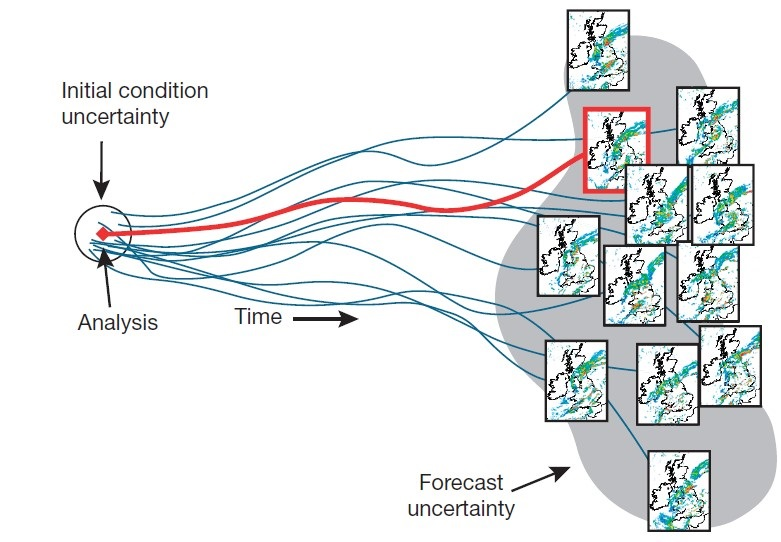
\includegraphics[scale=0.72]{figures/ensembleforecast_nature.png}
  \caption{集合预报概念示意图(摘自文献~\cite{bauer2015quiet})}
  \label{fig:ensenature}
\end{figure} 

\subsection{集合预报的扰动技术}
\subsubsection{初值扰动集合方案}
\label{sec:basictable}
气候系统模式的初值是由多个观测数据或者再分析资料同化得到的,其结果与真实的气候状态总是存在一定的差距。而气候系统模式又是典型的混沌系统,对于初始误差非常敏感。较小的初始误差在数值模拟的过程中,经过非线性叠加都会导致模拟结果具有非常大的差异。这也是著名的蝴蝶效应的由来。针对以上这两点,初值集合方法被用于天气和气候的预测当中。此方法的思想是从不同的初值状态开始启动预报,利用初值集合预报的结果来改善由于单一初值在混沌系统中形成的预测误差。现有的初值集合扰动方案大多数都是针对天气的,面向气候的集合技术研究还仍然在起步阶段。初值扰动方案获取扰动的基本原则有以下两个方面:一是要保证扰动场与用于预测的初始场的误差分布尽可能相似,这样才能保证每一个集合成员的初始场都有可能是真实的天气气候的初始状态,二是每一个扰动场在模式的模拟演进过程中,误差应该得以不断地发散,以保证集合成员最大可能包含实际的天气气候演进过程~\cite{陈静2002集合数值预报发展与研究进展}。

\subsubsection{模式扰动集合方案}
气候系统模式是由动力框架和物理过程共同组成的,次网格尺度的物理过程多是由统计分析得到,每个分量模式的物理过程也是在不断的发展中。模式结构的不确定性催生了模式扰动集合方案。通常的集合方法有:在模式的非绝热强迫项中加入随机噪声~\cite{buizza1999stochastic,berner2009spectral}以及选择不同的物理参数化方案作为集合成员~\cite{houtekamer1996system}等。研究表明,当前模式扰动集合方案最多的还是参数化方案的扰动,而参数化方案的个数毕竟有限,所以通常模式扰动集合方法需要配合初值扰动集合方案一起使用。

\subsection{多模式扰动的超级集合方案}
因单一气候模式在各种气候问题的表征上难以都达到行业前沿的水平,因此目前国际上也在设计多模式扰动集合预报系统以吸收多个优秀气候系统模式的优点~\cite{mylne1999quasi,evans1997joint}。但是相对于单一气候系统模式而言,多模式集合扰动的理论和技术方法还不够成熟,且在长期气候模拟上,多模式集合预报所需要的计算资源更多,计算代价更高。

\subsection{集合预测面临的问题及已有工作}
针对复杂气候系统模式的集合预测技术研究存在着巨大的挑战。主要有以下几个方面:

1. 气候系统模式中不确定参数问题严峻。气候系统模式由不确定性参数而导致的性能变化是多峰,非线性极强的空间~\cite{zhang2015automatic}。IPCC第五次报告中指出仅由参数不确定性变化而导致的气候系统模式模拟的全球平均温度差异可以达到2摄氏度左右。为了准确地模拟气候状态,对气候系统模式进行参数不确定性分析是十分重要的环节。

现有的不确定性分析方法主要分为前向的不确定性分析和反向的不确定性分析。下面将对这两类方法分别介绍。

前向的不确定性分析方法其核心思想是通过设计实验以及定量分析结果的统计特征等增加对问题本身的了解。主要的方法有采样、敏感性分析、构建代理回归模式等等~\cite{neelin2010considerations}。在不确定参数空间中进行采样,通过对采样点的评估,估计参数后验分布可能的情况。其方法可以是蒙特卡罗采样,单参数扰动采样,拉丁超立方采样,以及自适应采样等。敏感性分析是指通过对参数的扰动来获取参数的灵敏度信息,如果一个参数扰动极小的幅度就会对评估结果产生较大的影响,那么就可以判定其为敏感参数。敏感性分析方法主要分为局部敏感性分析和全局敏感性分析。局部敏感性分析主要考虑的是参数的一阶效应。不考虑两个或多个参数之间的交互效应。而全局敏感性分析是要同时考虑一阶效应和交互效应的~\cite{saltelli1995sensitivity,song2015global}。一般在气候系统模式中参数之间的交互效应是极强的。构建代理模式是利用统计回归等方法构建类似原来复杂问题的简单模型,用简单模型代替复杂模型的运行~\cite{xu2018parameter,muller2015ch4}。

反向的不确定性分析方法不考虑问题的统计特征,不要求对问题的后验分布有很好的了解,主要是将每一次模型的运行结果与观测进行对比,用对比结果来指导下一次参数的取值。主要的方法是数值优化方法。数值优化方法有传统的优化方法和进化优化方法等。传统的数值优化方法有单纯形下山方法、鲍威尔(powell)方法等,这些方法是局部优化方法,其特点是优化速度很快,能够快速收敛,但是在复杂多维的问题下容易陷入局部最优~\cite{severijns2005optimizing}。进化方法通过模拟种群进化的策略来不断更新样本,在种群中,根据物竞天择,适者生存的进化理论,只有表现好的样本能够以较大概率保留其基因到下一代。进化算法种类很多,例如协方差自适应调整进化策略(CMA-ES),差分进化(DE)等。它们主要的特点是克服陷入局部最优解的能力变强,但是需要的迭代次数也更多了,收敛性变差~\cite{auger2012tutorial,Storn1997Differential}。

上述提到的方法大都数都是为小应用而设计的,对小应用进行参数不确定性量化时对问题迭代多次求解,在时间和计算资源上也是可以接受的,但是像气候系统模式这种大应用,一次迭代需要很长时间,成百上千次的模拟显然在计算资源和时间上都难以接受。计算代价高的应用的不确定性分析对算法的性能和收敛性都提出了更高的要求~\cite{zhang2015automatic}。

2. 面向气候预测的初值集合扰动方法研究欠缺。初值扰动集合方法在天气预报中的应用已趋向成熟,但是针对更加复杂的气候系统模式来说初值集合预报方法还处在起步阶段。

通常用于天气预报的初始扰动集合方法包括蒙特卡罗随机方法、滞后平均法、奇异向量法和增长模繁殖法等。蒙特卡罗随机方法是对于初值做随机的微小扰动,用扰动后的初值分别进行模拟得到不同的模拟结果,其主要的缺点是随机扰动可能与真实初始场的误差并不相符,不好把握扰动的力度。滞后平均法获取初值扰动的方法是通过将从起报时间往后滞后若干天,例如第一个集合是起报日期,第二个集合就是起报日期往前推3天,第三个集合就从起报日期往前推6天,其他的集合起报日期依次类推。滞后平均法主要是利用了相近时间天气的状态相似性来组成了多个近似的初值扰动~\cite{hoffman1983lagged}。

蒙特卡罗随机和滞后平均法(LAF)实现相对简单,但是都缺乏较强的理论基础。在此基础上奇异向量法(Svs)和增长模繁殖法(BGM)方法相继被提出。奇异向量法由Buizza和Palmer首先提出的,该方法使用切线模型及其伴随向量计算奇异向量。用最大奇异值对应的奇异向量作为增长最快的扰动。该方法从1996年开始在欧洲中期天气预报中心得到使用~\cite{molteni1996ecmwf}。BGM是方法是Kalnay和Toth提出的,此方法在客观分析场上叠加随机扰动,进行预报,将控制预报减去扰动预报的差值调整后,作为下一次计算的扰动量,如此循环反复使用,最终形成初始场。此方法提供了对最快的可持续增长误差的估计,并代表了误差进展的可能方向~\cite{toth1997ensemble}。

尽管BGM和SVs集合方法在天气预报中得到广泛的应用,但它们很少用于气候预报。主要原因是SVs方法生成初始扰动的方法十分复杂,一般需要用到伴随模式,且在气候系统模式中需要极高的计算资源。而BGM方法由于高频噪声增长速度过快,导致增长模的增长率快速达到饱和,无法完全捕获气候系统模式中的一些慢变化过程的特征。因此,在许多国际前沿季节气候预报系统,如NCEP气候预报系统第2版(CFSv2)~\cite{saha2014ncep}以及北京气候中心的季节预报~\cite{liu2014relationships}中的集合策略仍然使用滞后平均法(LAF)。但是由于气候一直处在一个动态变化的过程中,对于初始场误差的表征仅仅用之前的状态来作为扰动显然是不够的。

%近几年,针对亚季节到季节时间尺度的气候预测集合方法的研究相继出现。 Kug等人。 (2010)将经验SVs方法应用于混合耦合模型的ENSO预测,并表明该方法可用于CGCM中的季节预测~\cite{kug2010new}。 Johanna和Piontek表明,与LAF方法相比,在ECHAM5 / MPIOM耦合气候系统模型的模拟中,在海洋组件中实施BGM可以改善温度和盐度的集合扩散~\cite{}。在Hudson等人的研究中。 (2013)和Kang等人。 (2014),通过在气候系统模型的季节预报系统中使用育种方法,改进了Madden-Julian Oscillation(MJO)的预测技巧。
%
气候系统模式本身的复杂度很高,加上集合也是高计算代价的策略,对于气候系统模式集合方案的研究进展相对缓慢。目前的初值集合方案大多数是针对天气模式建立的,在气候系统模式中如何提高集合模拟精度的问题一直存在。


3. 集合集成方法有待改进。因为集合预报多个成员的预报结果有一定的离散度,各个成员的预报分布并不相同,另外由于气候系统模式的系统偏差等原因,集合预报集成结果改进的空间很大。

当前确定性集合集成最常用的方法仍然是集合平均的方法。然而在气候系统业务预报中通常每月都会开始启动向前几个月的气候预测,每次有多个集合成员。如此众多的信息如果只用来做集合平均的话对计算资源是一种浪费。针对这一问题,基于模型数据和观测数据融合的集合集成技术正在悄然发展。其主要思路是将模式的输出结果与观测结果做对比,找出模式出现偏差的趋势,在真正做预测的时候将模式预测结果去掉这个趋势。常用的方法有概率匹配平均法,相似度集成法,最优百分位集成法等。

概率匹配法是将各个成员的空间分布按照优劣排序,空间分布结果越好的其集合权重系数越高,反之权重系数越低~\cite{ebert2001ability}。相似度集成法是将各个集合成员的空间分布的相似性作为评价标准,相似性越高则成员权重系数越高~\cite{陈力强2005短期集合预报中定量降水预报集合方法初探}。最优百分位法是利用历史数据提高不同等级的集成结果。例如不同降水等级有不同的集合成员及其权重系数~\cite{代刊2016中短期数字化天气预报技术现状及趋势}。

由此可见当前的集合集成方法多为统计分析法,随着集合成员数的增多,模式模拟时长的增加,更多的气候数据被积累,数据量越来越大,此时传统的集成方法就力有不逮,不能充分的使用已有数据。所以集合集成方法需要进一步改进。

\section{本文研究的主要内容}
\subsection{本文的研究内容和主要贡献}

针对当前气候预测中集合预报技术面临的问题,本文设计了一种结合参数优化的初值集合方案,其主要流程是针对气候系统模式的参数不确定性对物理过程中的参数进行优化,利用优化参数后的模型为集合预报打下良好的基础。在改善后的模型上设计了初值不确定性方案,并进一步开展集合集成技术的研究以改进确定性预报的性能。本文的主要研究内容和贡献有以下几个方面:

1.面向气候系统模式的高效参数优化方法。本文针对气候系统模式的高计算代价和强非线性等特点设计了基于多层感知机神经网络的代理模式参数优化方法:利用代理模式来估计下一个最优采样点,每增加一个采样都更新寻优策略。该方法相比进化优化算法的种群更新策略能够使得优化过程计算量更小,收敛速度更快,而相对于基于传统统计回归代理方法的模型,基于多层感知机神经网络的代理模式更适合复杂问题代理模型的构建。另外本文利用此优化思路构建了单目标优化算法、多目标优化算法和有约束优化算法并在复杂数学函数和单柱大气模式的优化试验中验证了所提出算法的有效性。

2. 面向气候预测的初值集合方案设计。针对气候系统模式初值集合方案存在的问题,设计了基于增长模繁殖法的集合方案,并对比了该方案与国家气候中心现用的LAF方法的预测效果。基于BCC-CSM(Beijing Climate Center Climate System Model)模式的对比结果显示,新设计的BGM方案比原方法在第一个月的性能提升非常显著。

3.结合参数优化的初值集合方案设计和应用。结合参数优化和初值集合方案,本文设计了一种面向气候预测的BGMOPT集合方法,并将其在BCC-CSM模式2008年12月至2009年3月的降雨预报中与原LAF方法进行对比。结果表明此方法在降雨预测中比原LAF方法更优。

4. 基于机器学习的集合集成技术研究。确定性预报需要对集合成员的结果做集成,但是现在最常用的气候预测集成方法还是集合平均法,本文设计了一种基于机器学习的集成技术,此技术利用了观测数据和已有模式输出的大量数据对模式集合预测结果进行集成修正。修正后的模式预测能力相对原集合平均法改进32\%。

5. 气候集合预测系统设计与实现。综合以上内容,本文设计了面向气候的集合预测系统。此系统中包括了不确定参数的优化、初值扰动方案的设计、集合预测的模拟过程、集合结果集成修正等模块,实现了自动化的气候预测与结果分析。

\subsection{本文的组织架构}
本文共5个章节,每一章的具体内容如下:

第1章首先介绍了研究背景和意义,简述了气候系统模式的工作原理及其发展历程,然后介绍了集合预报的概念及其常用方法。最后针对气候系统模式集合预测存在的问题展开讨论并总结了已有的工作。

第2章首先介绍了气候系统模式参数优化问题,然后描述了各类问题的当前常用方法和本文提出的方法。并将常用方法和本文方法在单柱大气模式和复杂数学函数上进行了测试和对比。最后介绍了各类优化算法的整合和简要的实现过程。

第3章首先介绍了当前面向气候的集合初值扰动方案存在的问题。然后介绍了天气中的常用的初值集合方法BGM的流程,并解释了为何它不适用于气候系统模式。然后针对气候预测的特征,重新设计了面向气候预测的BGM方法,并将其与国家气候中心所使用的LAF在BCC-CSM模式上做了对比。

第4章首先介绍了本文所提出的结合参数优化的初值集合方法,然后针对当前集合集成方法未能充分应用大量已有模式输出数据和观测数据的问题,提出了基于机器学习的集合预测修正技术,最后本文描述了包含自动参数优化、初值扰动生成、集合预报、集合集成等模块的综合集合系统设计与实现,并叙述了该系统在BCC-CSM模式上的应用案例。

第5章是全文的总结,并提出了下一步工作的方向。
%\chapter{地球系统模式面临的不确定性问题}
\label{cha:intro}

\section{论文的背景与意义}
2018年IPCC发布全球升温1.5摄氏度特别报告,报告指出,应该将全球变暖限制在1.5摄氏度,相比之前提出的限制在2摄氏度可以显著减少对气候变化的影响,而过去一个世纪,全球已升温1摄氏度,在全球变暖的背景下,寒潮、龙卷风、干旱、暴雨、暴雪,火灾等极端气候事件加剧。特别是近几年来,极端事件的频发,对人类的生命和财产都造成了不可挽回的损失。例如2016年我国暴雨频发,共出现46次区域暴雨,26个省(区、市)出现城市内涝;在非洲之角,2017年1月至2月严重的干燥季节以及3月至5月降雨极少的雨季,索马里超过半数的耕地遭受旱灾;2018年加利福尼亚遭受的毁灭性的野火是美国一个多世纪以来最致命的火灾。这些极端天气的出现,气候问题的逐渐凸显,如此现状为气候模拟预测提出了严峻的挑战。

地球系统模式作为模拟天气气候的数值模拟模型,是模拟预测未来气候的强有力的工具。它是通过建立数学物理方程组来模拟地球系统中大气、海洋、陆面、海冰和生态等各个圈层内的动力、物理和化学等复杂过程以及圈层间的水汽、能量和物质的交换过程。地球系统模式模拟的过程比一般气候系统模式更复杂,包括了大气环流、太阳辐射、陆面水文、植被、海洋海冰、气溶胶和人类活动等,地球系统模式模拟的准确性决定着气候预测的预报能力。

气候系统预测的不确定性是导致模拟不准确性的主要原因。其主要有地球系统模式的不确定性、温室气体等排放场景的不确定性,以及气候系统的内部变率的不确定性。IPCC会议对排放场景的不确定性的处理是设计多个排放场景,在不同的场景下对气候进行预测,对于内部变率的不确定性会随着模拟的时长而不断减少,所以目前亟待研究的是地球系统模式的不确定。地球系统模式的不确定性是气候模拟准确与否的决定性因素。地球系统模式的不确定性又分为模式结构的不确定性、边界条件不确定性、初始条件不确定性和物理参数不确定性。模式结构的不确定性是由于地球系统模式由大气、海洋、海冰、陆地等多个模块组成,每个模块都在不断的发展过程中,模式在构建的过程中也存在着大量的假设和近似操作,每个模块都还在研究之中,与真实的情况存在着巨大的差异,还有待深入的研究,理论也尚未成熟。边界的不确定性指的是模式的边界情况十分复杂,模拟的边界会对模拟产生巨大的影响,例如大气模式的下边界由地形状况、人类活动、生态环境等构成,而大气模式的上边界也包括太阳活动等。这上下边界都会对大气模式的模拟产生巨大的影响。初始条件的不确定性指的是气候模拟初始场的不确定性,由于洛伦兹提出的蝴蝶效应可知,初始场微小的差异将会引起模拟结果的不同,而物理参数化的不确定性则指的是地球系统模式中的物理参数化过程中存在着很多不确定性参数,这些参数是由专家根据经验而人为设定的,而地球系统模式的每个模块中都存在着大量的不确定性参数,这些不确定性参数也决定了模式准确性与否。

集合预报技术是一种针对地球系统模式不确定性分析的重要策略。其方法的原理是利用多个集合预测来代替原有的单一预报。集合预报已在各大预报中心得到应用。常用的方法有参数集合预报以及初值集合预报。
参数集合是
初值集合预报是

集合预报所面临的问题
(1)地球系统模式中的参数不确定性问题
(2)初值不确定性问题
(3)
本文主要关注的是初始条件的不确定性和物理参数的不确定性,这也是目前阶段最急需解决的不确定性问题。初始条件的不确定性的解决方案是利用同化和集合等方法。

当前针对不确定性分析的方法有前向的不确定性分析方法和反向的不确定分析方法。

\section{当前的不确定性分析方法}
\label{sec:first}
面对参数的不确定性问题,我们可以用现有的不确定分析方法。现有的不确定性分析方法主要分为前向的不确定性分析和反向的不确定性分析。下面将对这两类方法分别介绍

(1)	前向的不确定分析方法

前向的不确定性分析方法其核心思想是通过设计实验以及定量分析结果的统计特征等增加对问题本身的了解。主要的方法有采样、敏感性分析、构建代理回归模式等等。在不确定参数空间中进行采样,通过对采样点的评估,估计在参数空间中后验分布可能的分布情况。其方法可以是蒙特卡罗采样,单参数扰动采样,拉丁超立方采样,以及自适应采样等等。敏感性分析是指通过对参数的扰动来获取参数的灵敏度信息,如果一个参数扰动极小的幅度就会对评估结果产生较大的影响,那么就可以判定其为敏感参数。敏感性分析方法主要分为局部敏感性分析和全局敏感性分析。局部敏感性分析主要考虑的是参数的一阶效应。不考虑两个或多个参数之间的交互效应。而全局敏感性分析是要同时考虑一阶效应和交互效应的。一般在地球系统模式中参数之间的交互效应极为强烈的。构建代理模式是利用统计回归等方法构建类似原来复杂问题的简单模型,用简单模型代替复杂模型的运行。

(2)	反向的不确定性分析方法

反向的不确定性分析方法不考虑问题的统计特征,不要求对问题的后验分布有很好的了解,主要是通过每一次模型的运行结果与观测进行对比,用对比结果来指导下一次参数的取值。主要的方法是数值优化方法。数值优化方法有传统的优化方法有进化的优化方法等。传统的数值优化方法有单纯形下山方法、powell方法等等,这些方法是局部优化方法,其特点是优化速度很快,能够快速收敛,但是在复杂多维的问题下容易陷入局部最优。进化方法通过模拟种群进化的策略来不断更新样本,在种群中,根据物竞天择,适者生存的进化理论,只要表现好的样本能够以较大概率保留其基因到下一代。

进化算法种类很多,例如CMA-ES,DE,GA等等,其主要的特点是克服陷入局部最优解的能力变强,但是其需要的迭代次数也更多了,收敛性变差。

\section{当前的初值集合方法}
\label{sec:basictable}
由于数值气象模式对初始误差非常敏感,较小的初始误差经过数值模拟,误差经过非线性叠加将会导致结果具有非常大的差异。这也是著名的蝴蝶效应的由来。初值不确定性问题目前主要的解决方案是数据同化和集合的方法。数据同化是为天气气候模式提供更高质量的初值的方法。它是通过将不同分分辨率、不同来源、不同误差信息的观测数据融合到初值当中去。通过做初值对观测的不断逼近来获取更优的初值。而初值的不确定性对天气和短期的气候模拟有非常大的影响,初值的质量将影响着最后的预报质量。目前常用的方法有卡尔曼滤波方法。而集合的方法主要是利用多个集合成员从多个不同的初值起报,用多个成员的结果来共同决定预报结果。质量再好的初值都有可能与真实的天气和气候存在着一定程度的差异,这个时候用集合的方法能更好的避免由于初值误差而导致的模拟的不准确定性。

目前用于气候的集合方法比较少见,还处在研究的初级阶段。而对于天气的集合方法主要有蒙特卡罗随机方法、滞后平均法、奇异向量法和增长模繁殖方法。
蒙特卡罗随机方法是对于初值做随机的微小扰动,用扰动后的初值分别进行模拟得到不同的模拟结果,其主要的缺点是随机微小的扰动可能与真实天气存在着较大的误差,不好把握扰动的力度。而滞后平均法主要是通过将从起报时间往后滞后N天,例如第一个集合是起报日期,第二个集合就是起报日期往前推3天,第二个集合就从起报日期往前推6天,其他的集合依次类推。滞后平均法主要是利用了相近时间天气的

\section{面临的主要挑战}
\label{sec:theorem}
对复杂多维高峰的地球系统模式做混合集合方案设计存在着严峻的挑战。主要有以下几条:(1)地球系统模式是运算代价极高的应用程序;(2)地球系统模式本身复杂非线性强;(3)现有的不确定性分析大多数针对小应用;(4)面对气候系统模式的集合方案设计较为欠缺。

(1)地球系统模式包括大气、海洋、海冰、陆面等过程,由复杂的动力学热力学等方程组构成,运行一次需要极高的计算代价。例如CESM,世界上著名的地球系统模式,2度分辨率的AMIP实验的全球模拟180进程,至少需要10小时,而在如此计算代价高的模式上做优化参数后的集合设计十分困难。首先参数优化前面提到的方法大多数也是需要上百次迭代才能寻找到合适的参数组合,而对于初值集合来说,目前的初值集合方案需要的集合成员数大概都在10个成员以上,这又进一步增加了地球系统模式的混合集合集成方案设计的难度。

(2)地球系统模式本身不确定性参数而导致的性能变化是多峰,非线性极强的空间。且在这种不规则的空间内还有很多参数组合可能会导致模型中某些必须要满足的物理约束没有被满足,比如说,在AMIP实验中,大气顶进出的能量应该一致,才能在保证模式长期模拟是在一个能量守恒的前提下进行的。但是不确定参数设置不合理也会导致能量平衡被破坏。在如此复杂的参数空间中进行参数寻
(3)上面介绍了现有的参数不确定性分析工具,这些工具大都数都是为小应用而设计的,对小应用进行参数优化迭代进行多次在时间和计算资源上也是可以接受的,但是大应用如果一次迭代需要很长时间,成百上千次的模拟显然是对计算能力和等待时间上都难以接受,提出了更高的挑战。
(4)气候系统模式的集合方案较为欠缺。集合本身就是高计算代价的方法,加上气候系统模式本身的复杂度很高,对于气候系统模式所做的集合方案研究还处于初级阶段。目前的初值集合方案大多数是针对天气模式建立的,在气候系统模式中如何提高集合模拟的精度的问题一直存在。

\section{本文研究的主要内容和贡献}
\label{sec:bib}
1.基于代理模式的参数优化平台
本文针对地球系统模式的高计算代价和强非线性等特点设计了参数优化平台,参数优化平台包括单目标优化、多目标优化和有约束优化。

2. 一种面向气候系统模式的集合方案设计
针对气候系统模式现存初值集合方案存在的问题,设计了面对气候的BGM初值集合方案,并对比了该方案与国家气候中心现用的LAF方法的差异。并设计了一套自动的集合评比方案。评比结果显示,我们新设计的方案比原来方法在第一个月的提升性能非常显著。气候中的降水、环流场和温度等都有明显的提高。

3. 集合集成方案研究
确定性预报需要对集合成员的结果做集成,但是现在最常用的集合方法还是集合平均法,本文针对不同的集成目标提出了两种集合集成方法,并将两种方法与原有的集合平均法做了详细的比较,证明了新方法比原有方法的集成精度更高。

4. 混合集合集成系统
结合参数优化和初值集合方案,我们设计了混合集合集成系统。该系统包括了不确定参数的调整,初值扰动集合方案的设计,以及最后的集合集成系统。



\subsection{国内外集合预测系统概况}
美国NCEP的集合预测系统由多个
欧洲中心的
日本气象厅的
我国的国家气候中心的气候预测的业务系统主要是由LAF方法


指标相关性分析如下:
\begin{table}[htb]
\centering
\caption{MJO指标独立性检验}  
\begin{tabular}{llll}  
\toprule[1.5pt]
\centering
  & sc\_w & sc\_s & sc\_l  \\  
\hline  
    sc\_w    & 1        & 0.45     & 0.53 \\
    sc\_s    & 0.45     & 1        & 0.32 \\
    sc\_l    & 0.53     & 0.32     & 1 \\
\bottomrule[1.5pt]  
\end{tabular}  
\end{table}



\begin{figure}
\begin{minipage}{0.48\textwidth}
  \centering
  \includegraphics[height=2cm]{figures/cntl.phase-lon.png}
  \caption{并排第一个图}
  \label{fig:parallel1}
\end{minipage}\hfill
\begin{minipage}{0.48\textwidth}
  \centering
  \includegraphics[height=2cm]{figures/cntl.u850.wavefreq.winter.png}
  \caption{并排第二个图}
  \label{fig:parallel2}
\end{minipage}
\begin{minipage}{0.48\textwidth}
  \centering
  \includegraphics[height=2cm]{figures/cntl.olr.wavefreq.winter.png}
  \caption{并排第二个图}
  \label{fig:parallel2}
\end{minipage}
\end{figure}



\begin{figure}[H]
\begin{minipage}{0.28\textwidth}
  \centering
  \includegraphics[scale=0.1]{cntl-phase-lon.png}
  \caption{并排第一个图}
  \label{fig:parallel1}
\end{minipage}\hfill
\begin{minipage}{0.28\textwidth}
  \centering
  \includegraphics[scale=0.1]{cntl-u850-wavefreq.winter.png}
  \caption{并排第二个图}
  \label{fig:parallel2}
\end{minipage}
\end{figure}



边界的不确定性指的是模式的边界情况十分复杂,模拟的边界会对模拟产生巨大的影响,例如大气模式的下边界由地形状况、人类活动、生态环境等构成,而大气模式的上边界也包括太阳活动等。这上下边界都会对大气模式的模拟产生巨大的影响。

模式结构的不确定性是由于地球系统模式由大气、海洋、海冰、陆地等多个模块组成,每个模块都在不断的发展过程中,模式在构建的过程中也存在着大量的假设和近似操作,每个模块都还在研究之中,与真实的情况存在着巨大的差异,还有待深入的研究,理论也尚未成熟。

通常用于天气预报的初始化的集成方法包括奇异向量法和增长模繁殖法。奇异向量法是Buizza和Palmer在1995年提出的,该方法使用线性切线模型及其伴随向量计算奇异向量。用最大奇异值对应的奇异向量作为增长最快的扰动。SVs方法在欧洲中期天气预报中心得到使用(ECMWF, Molteni et al., 1996)。BGM是方法是Kalnay and Toth在1991年提出的,此方法在客观分析场上叠加随机扰动,进行预报,将控制预报减去扰动预报的差值调整后,作为下一次计算的扰动量,如此循环反复使用,最终形成初始场。此提供了对最快的可持续增长误差的估计,并代表了误差进展的可能方向。

尽管BGM和SVs集合方法通常用于天气预报,但它们很少用于季节预报。主要原因是SVs方法的生成初始扰动复杂,一般需要使用伴随模式,而其在气候系统模式中一般较难获得,且其需要极高的计算资源。而BGM方法由于高频噪声的缘故增长模增长速度过快,无法完全捕获气候系统模式中的一些慢变化过程的特征。因此,在许多国际前沿季节预报系统,如NCEP气候预报系统第2版(CFSv2)(Saha等,2014)以及北京气候中心的季节预报(Liu et al.2014)中的集合策略仍然使用滞后平均预测(LAF)。LAF方法从初始条件开始,一直滞后于预测时间的开始一个不同的量(Hoffman和Kalnay,1983)。这种方法在季节性预报中是可行的,特别是对于几十年的后报。然而,使用来自预测期之前的信息可能不够,因为气氛不断变化。

最近,一些研究提出了从亚季节到季节时间尺度预测的集合方法的改进。 Kug等人。 (2010)将经验SVs方法应用于混合耦合模型的ENSO预测,并表明该方法可用于CGCM中的季节预测。 Johanna和Piontek(2014)表明,与LAF方法相比,在ECHAM5 / MPIOM耦合气候系统模型的模拟中,在海洋组件中实施BGM可以改善温度和盐度的集合扩散。在Hudson等人的研究中。 (2013)和Kang等人。 (2014),通过在气候系统模型的季节预报系统中使用育种方法,改进了Madden-Julian Oscillation(MJO)的预测技巧。

目前,基于LAF集合的北京气候中心的季节预测仍然存在不足,特别是在亚洲季风区域(Liu et al。,2014,2015)。在BCC预测系统中应用不同的集成方法是提高其预测技能的解决方案之一。 SVs方法是最快的线性初始误差增长扰动方法(Cheng et al。,2010),但很难用于业务季节预测系统。与SV相比,BGM方法在计算成本上更经济并且更容易实现(Chikamoto等人,2007; Saito等人,2011)。


气候系统模式集合预测是降低气候预测不确定性,提升预报能力的重要方法。然而由于物理过程参数和初值的不确定性等原因导致气候预测存在严峻的挑战。本文提出了一种基于参数优化的气候系统模式初值集合方法。此方法首先对气候系统模式中的不确定性参数进行优化,然后将优化参数后的模式用于初值集合预测。

参数的不确定性严重影响了气候系统模式的模拟水平,但是目前的参数不确定性量化方法在复杂的气候系统模式上的应用需要极高的时间和计算成本,急需要快速高效的不确定性分析方法。本文提出了一组面向气候预测的基于ANN代理模式的参数优化方法,其中包括单目标优化,多目标优化和有约束优化。本文提出的优化算法与当前常用的优化算法在复杂数学函数和单柱大气模式上的评测结果表明,在大多数情况下,新提出的算法在性能和收敛性上具有优势。在单柱大气模式上,本文的多目标优化方法的收敛速度可相对NSGAIII方法的收敛速度提升6倍以上。

初值集合扰动方法的研究对降低初值的不确定性至关重要。然而当前最常用的滞后平均法缺乏一定的理论基础。本文提出了一种面向气候预测的增长模繁殖法,此方法是在面向天气预测的增长模繁殖法的基础上结合气候预测特征对初始繁殖扰动生成,繁殖循环长度等关键技术进行重构。本文将此方法与国家气候中心当前所使用的滞后平均方法在BCC-CSM气候系统模式上进行了评测。2000年到2014年的回报实验结果表明新提出的BGM方法在第一个月的大多数气候变量的预测中相比LAF方法的改进明显。500hpa位势高度相对于LAF方法改进了10\%。少部分变量的提升效果延伸至四个月。

最后本文将新提出的基于参数优化的气候系统模式初值集合方法在BCC-CSM模式上进行测试,以MJO和EASM为目标,以模式顶辐射平衡为约束对不确定性参数进行优化,将优化后的参数用于BGM初值扰动集合。结果表明新的集合方法在2008年12月到2009年3月的气候模拟中表现良好。四个月全球降水MSE相比原方法改进约15\%。另外为了进一步提升确定性预报结果,本文设计了一种基于机器学习的集合预测修正方法,此方法结合了观测和模式输出数据的特征对模式预测结果的进行修正。在13个月的SST预测中此方法可对相对于集合平均法改进10\%.


\begin{figure}[H]
\label{fig:u850freq}
\centering
\subfigure{
\begin{minipage}[t]{0.48\textwidth}
\centering
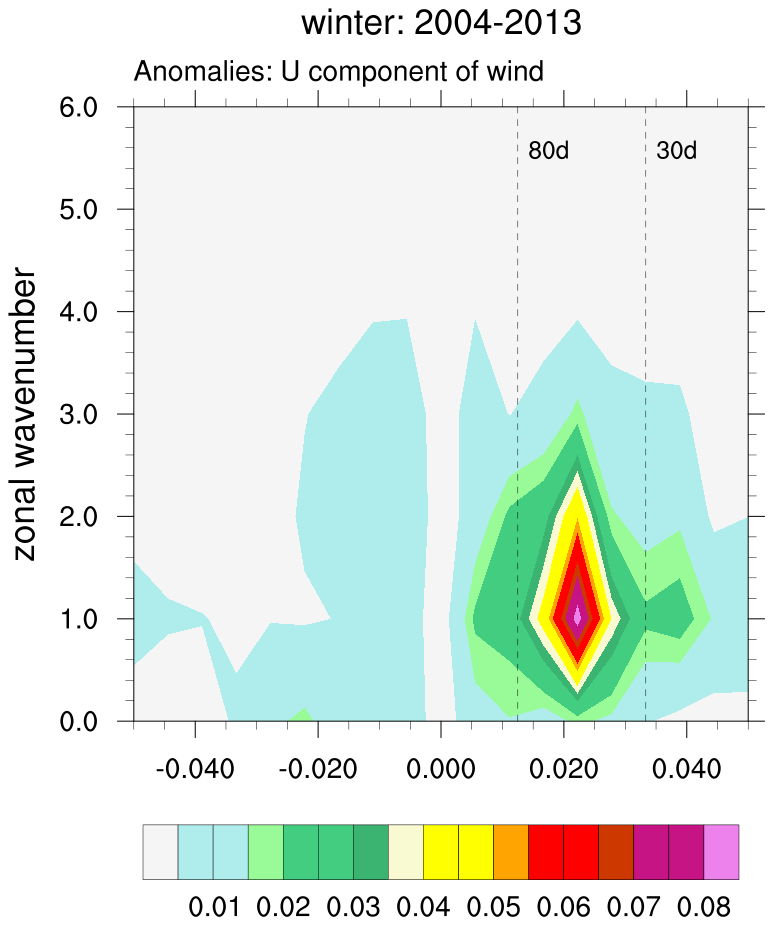
\includegraphics[width=6cm]{figures/obs-u850-wavefreq-winter.png}
\caption{MJO观测冬季U850波谱场}
\end{minipage}
\begin{minipage}[t]{0.48\textwidth}
\centering
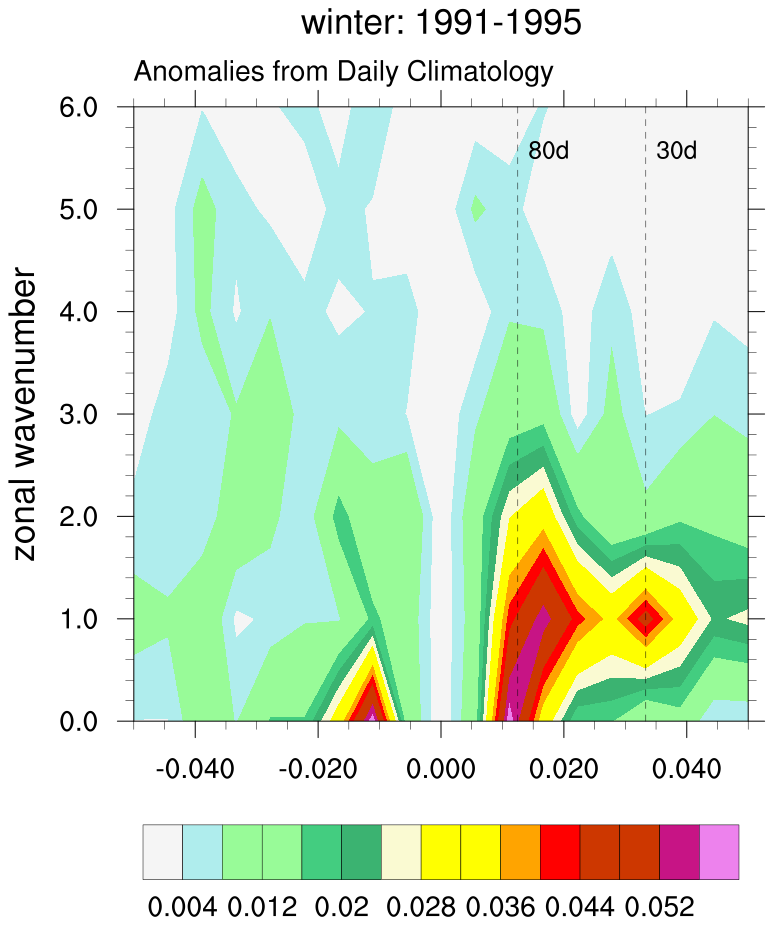
\includegraphics[width=6cm]{figures/cntl-u850-wavefreq-winter.png}
\caption{MJO控制预报的冬季U850波谱场}
\end{minipage}
}
\subfigure{
\begin{minipage}[t]{0.48\textwidth}
\centering
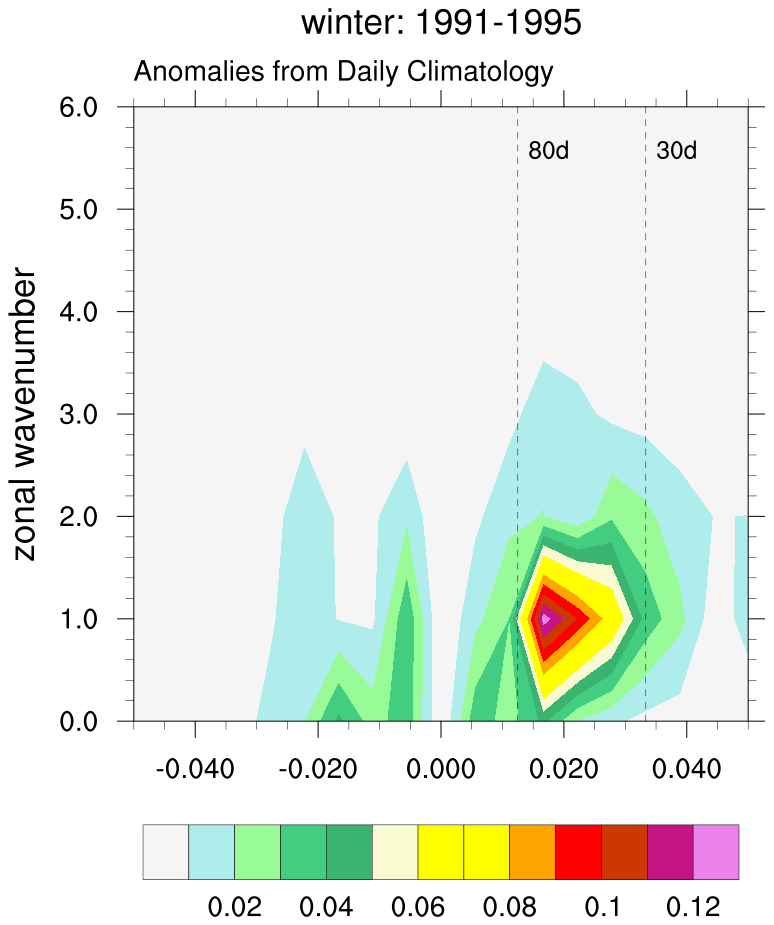
\includegraphics[width=6cm]{figures/runstandrad-u850-wavefreq-winter.png}
\caption{MJO优化参数后的冬季U850波谱场}
\end{minipage}
}
\end{figure}

\begin{figure}[H]
\label{8phase-lon}
\centering
\subfigure{
\begin{minipage}[t]{0.48\textwidth}
\centering
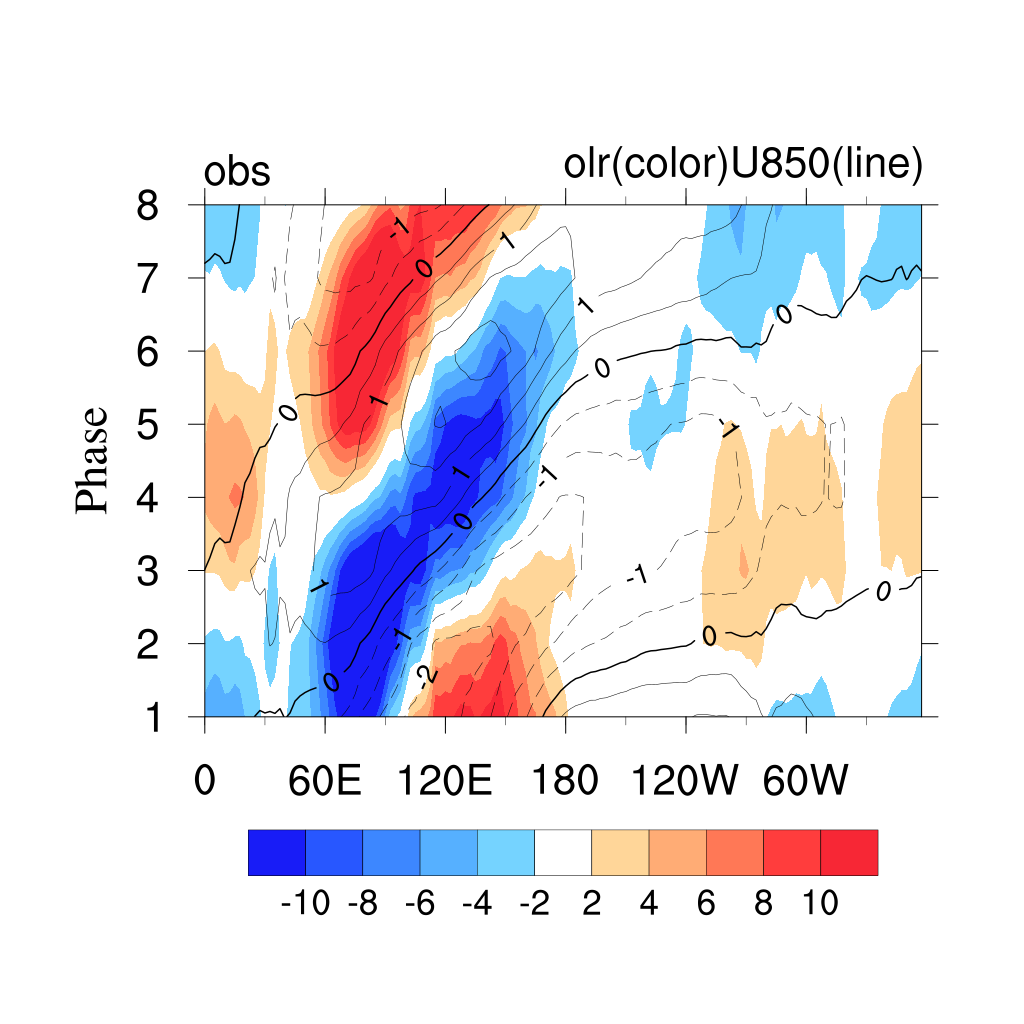
\includegraphics[width=8cm]{figures/obs-phase-lon.png}
\caption{MJO观测8位相合成图}
\end{minipage}
\begin{minipage}[t]{0.48\textwidth}
\centering
\includegraphics[width=8cm]{figures/cntl-phase-lon.png}
\caption{MJO控制预报的8位相合成图}
\end{minipage}
}
\subfigure{
\begin{minipage}[t]{0.48\textwidth}
\centering
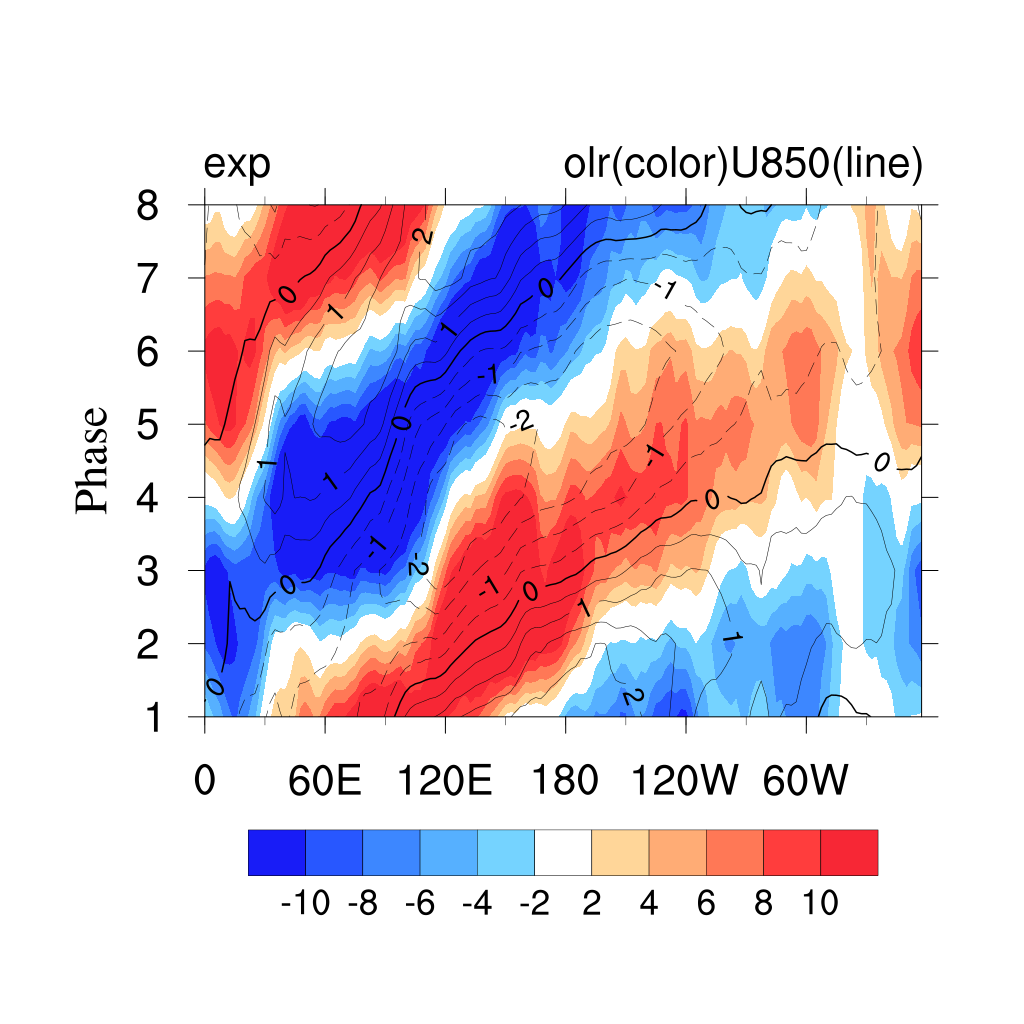
\includegraphics[width=8cm]{figures/runstandrad-phase-lon.png}
\caption{MJO改进参数后的8位相合成图}
\end{minipage}
}
\end{figure}

 \begin{figure}[H]
\centering
\begin{minipage}[t]{0.48\textwidth}
\centering
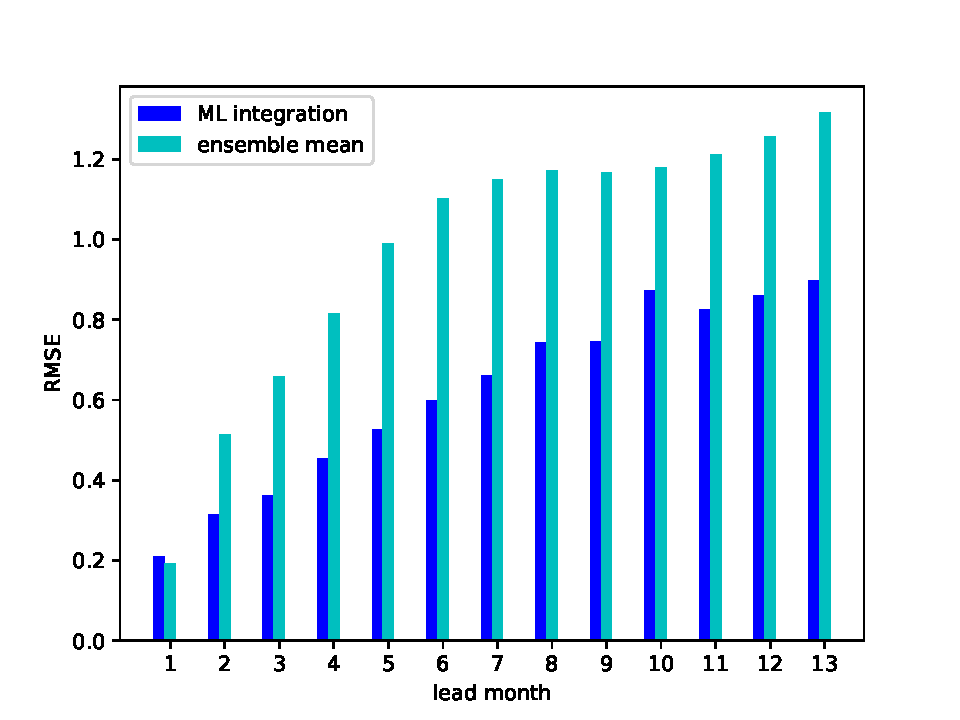
\includegraphics[width=8cm]{figures/RMSEensega.pdf}
%\caption{RMSE对比}
\end{minipage}
\begin{minipage}[t]{0.48\textwidth}
\centering
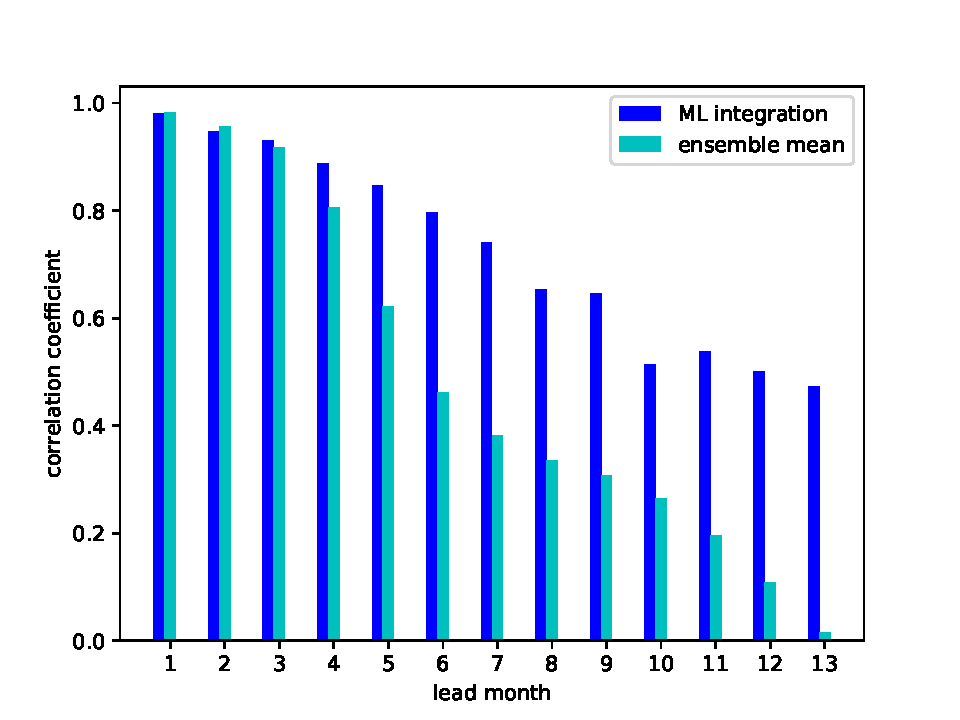
\includegraphics[width=8cm]{figures/RMSEensegacorr.pdf}
%\caption{相关系数对比}
\end{minipage}
\caption{机器学习修正方法与集合平均集成结果对比}
\end{figure}

\begin{figure}[H] % use float package if you want it here
  \centering
  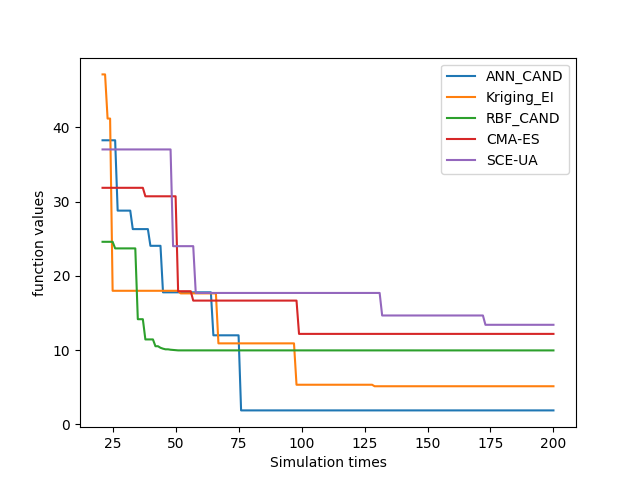
\includegraphics[scale=0.6]{figures/all_Rast4.png}
  \caption{单目标优化算法在Rastrigin函数上的优化结果}
  \label{fig:xfig1}
\end{figure}

\begin{figure}[H] % use float package if you want it here
  \centering
  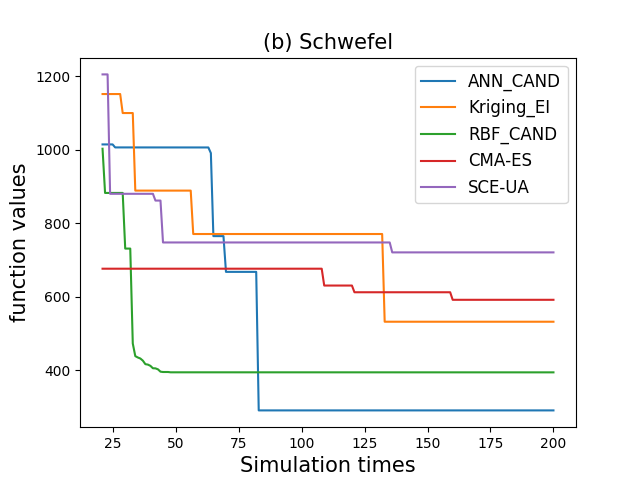
\includegraphics[scale=0.6]{figures/all_schw4.png}
  \caption{单目标优化算法在Schwefel函数上的优化结果}
  \label{fig:xfig1}
\end{figure} 

\begin{figure}[H] % use float package if you want it here
\label{prectresult}
  \centering
  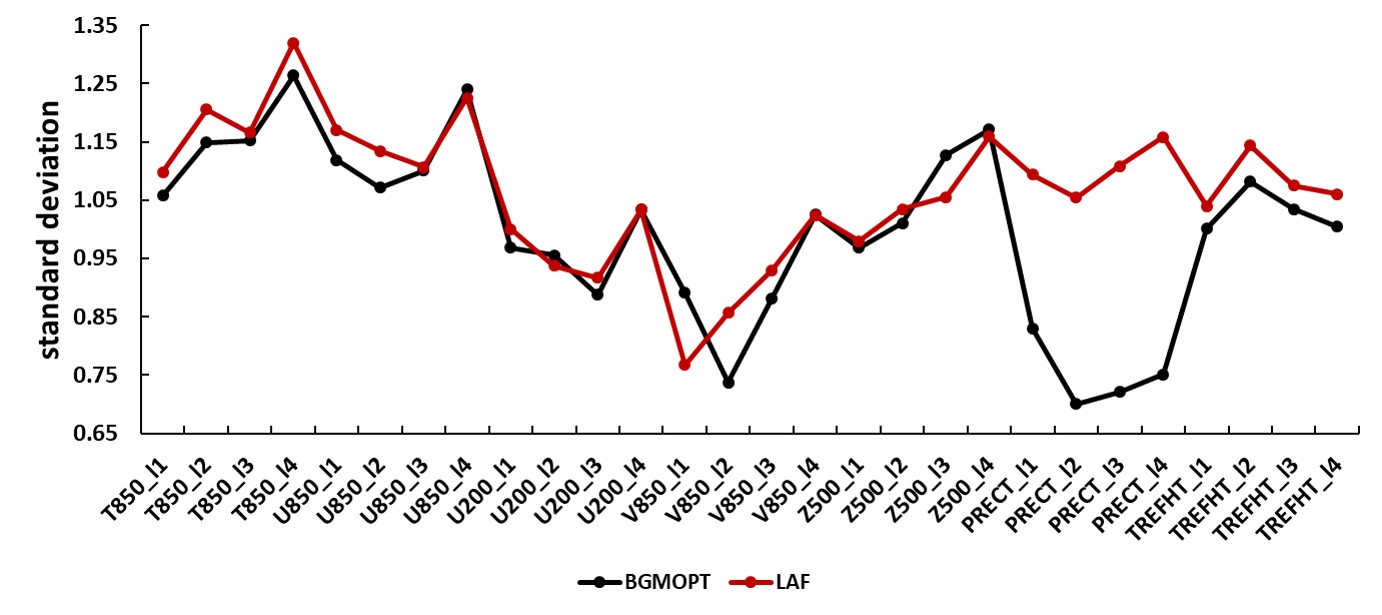
\includegraphics[scale=0.6]{figures/allvar-std.jpg}
  \caption{集合方法针对降水RMSE结果对比}
  \label{fig:xfig1}
\end{figure} 

\begin{figure}[H] % use float package if you want it here
\label{prectresult}
  \centering
  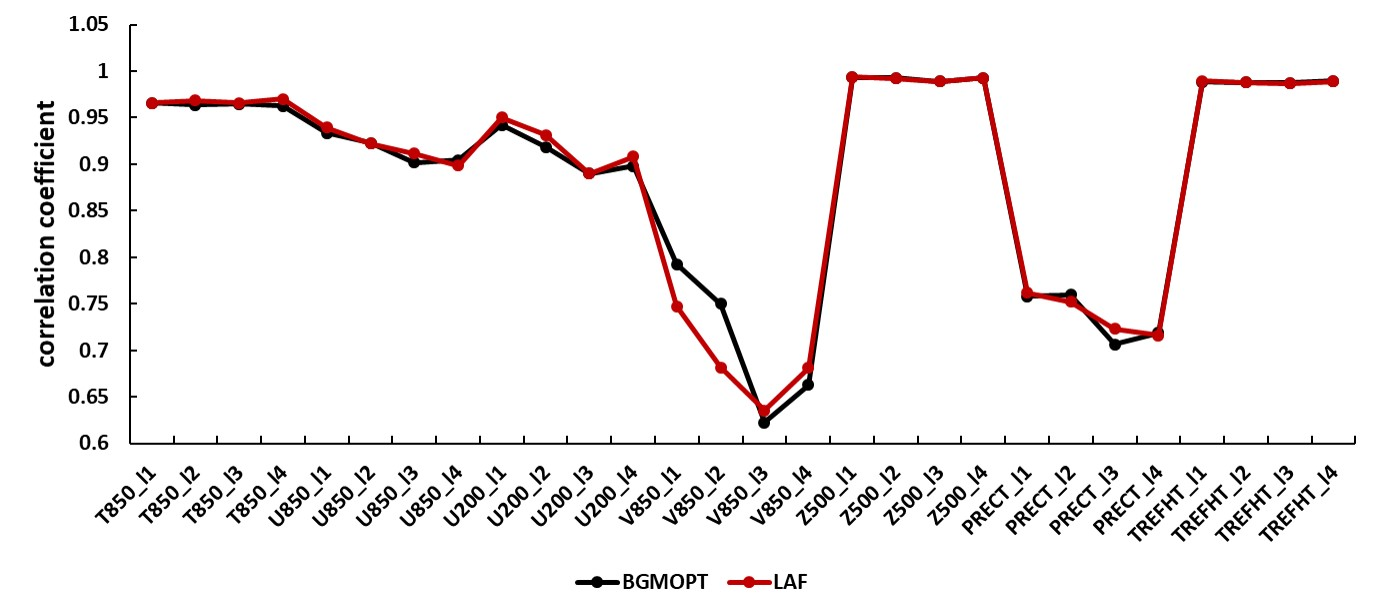
\includegraphics[scale=0.6]{figures/allvar_coef.jpg}
  \caption{集合方法针对降水correlation coefficient结果对比}
  \label{fig:xfig1}
\end{figure} 

\begin{figure}[H] % use float package if you want it here
\label{prectresult}
  \centering
  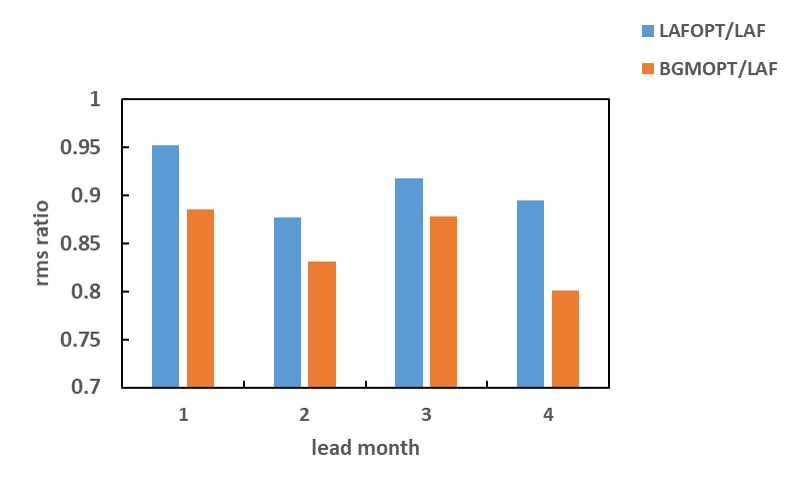
\includegraphics{figures/rmse-precip.jpg}
  \caption{集合方法针对降水RMSE结果对比}
  \label{fig:xfig1}
\end{figure} 

\begin{figure}[H] % use float package if you want it here
\label{prectresult}
  \centering
  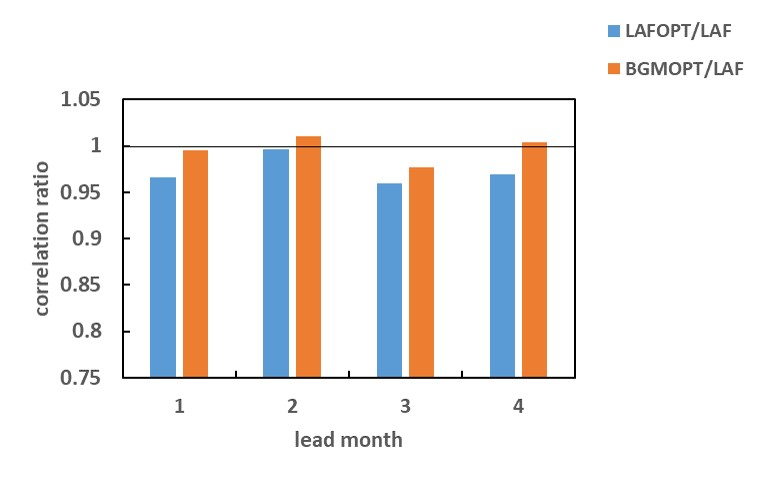
\includegraphics{figures/corr-precip.jpg}
  \caption{集合方法针对降水correlation coefficient结果对比}
  \label{fig:xfig1}
\end{figure} 

\begin{figure}[H] % use float package if you want it here
\label{Fig:easmresut}
 \centering
 \subfigure[集合集成方法的RMSE比较]{
 \centering
    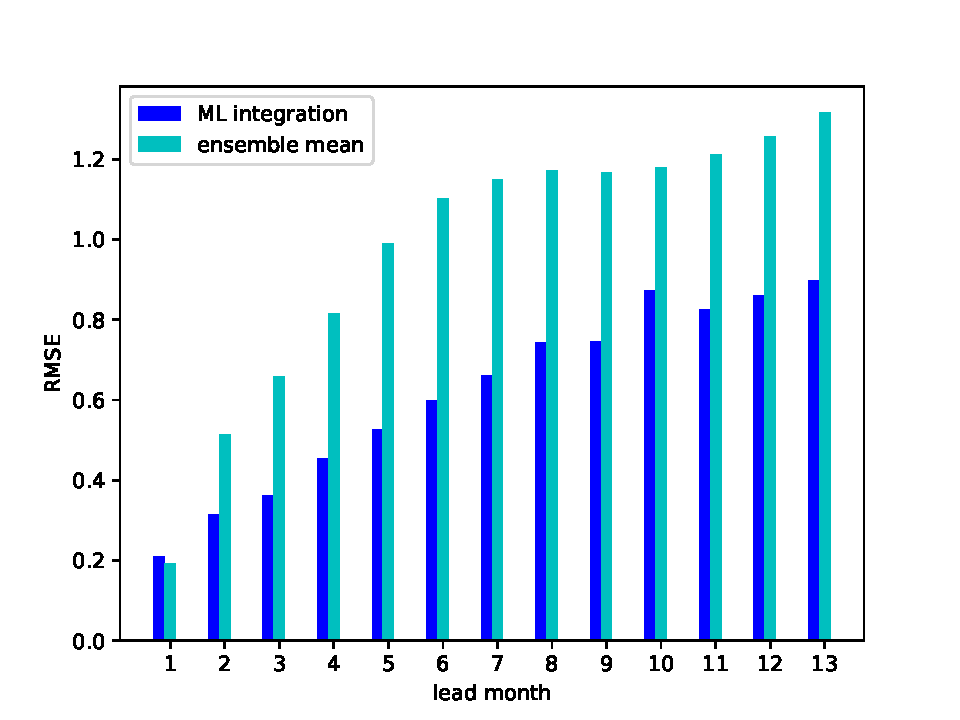
\includegraphics[scale=0.55]{figures/RMSEensega.pdf}
}

 \subfigure[集合集成方法的相关系数的比较]{
 \centering
     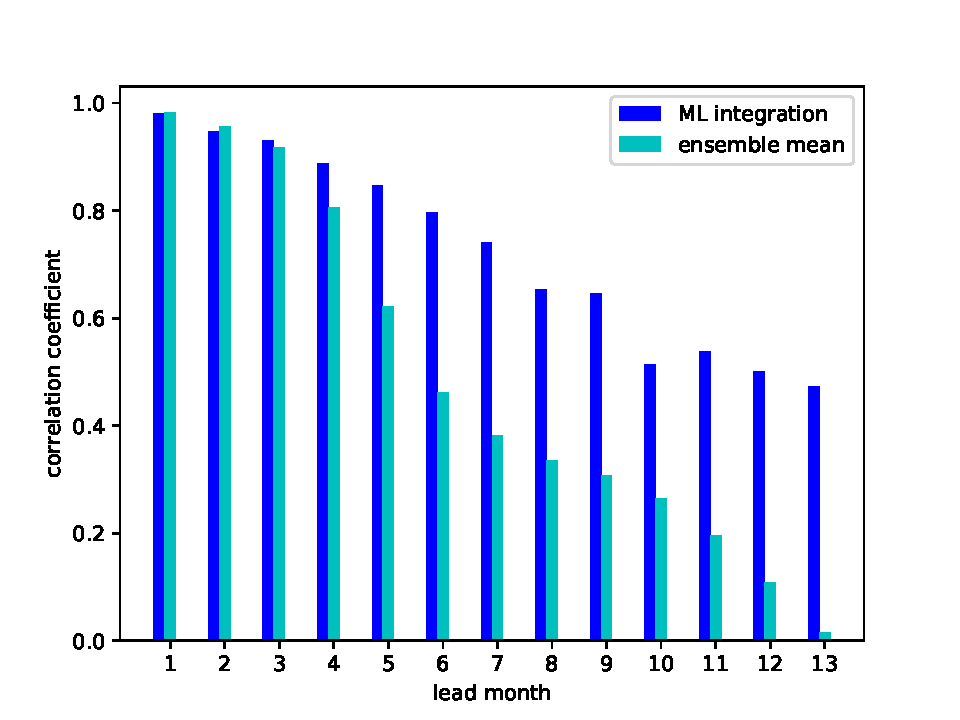
\includegraphics[scale=0.5]{figures/RMSEensegacorr.pdf}
 }
 \caption{机器学习修正方法与集合平均集成结果对比}
 \end{figure}

\begin{figure}[H] % use float package if you want it here
  \centering
  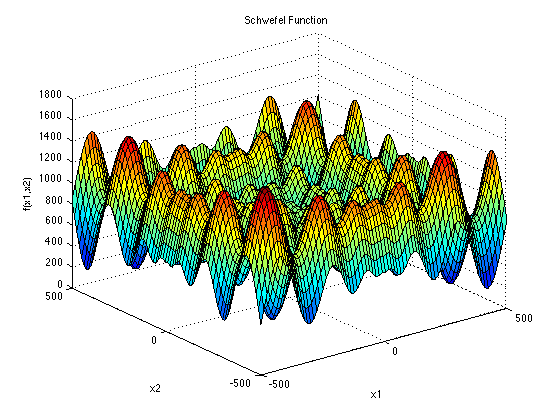
\includegraphics[scale=0.5]{schwef.png}
  \caption{Schwefel函数二维空间图}
  \label{fig:xfig1}
\end{figure}

\begin{figure}[H] % use float package if you want it here
  \centering
  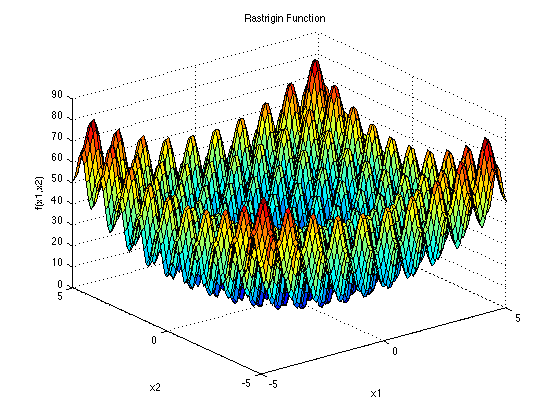
\includegraphics[scale=0.5]{rastr.png}
  \caption{Rastrigin函数二维空间图}
  \label{fig:xfig1}
\end{figure}

\begin{figure}[H] % use float package if you want it here
  \centering
  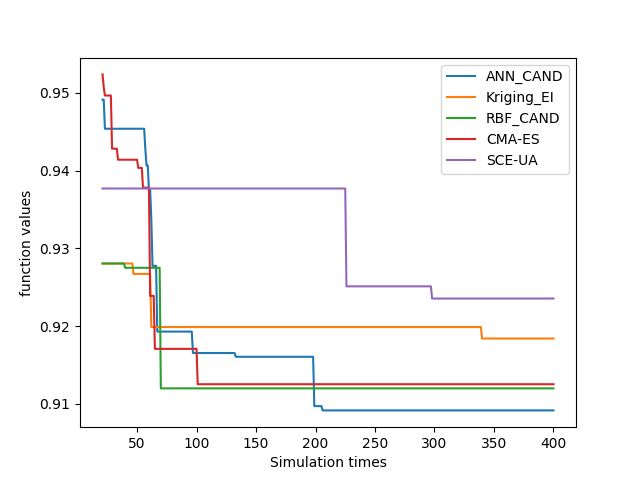
\includegraphics[scale=0.6]{figures/all_scam_new.png}
  \caption{单目标优化算法在TWPSCAM上的优化结果}
  \label{fig:xfig1}
\end{figure} 

\begin{figure}[H] % use float package if you want it here
  \centering
  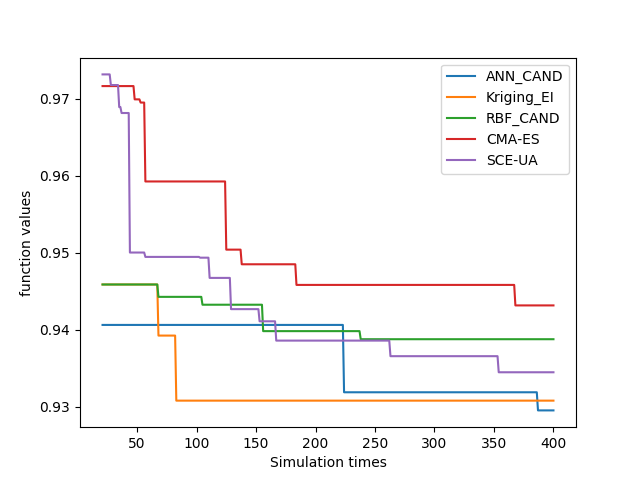
\includegraphics[scale=0.6]{figures/all_scam_ARW.png}
  \caption{单目标优化算法在MPSCAM函数上的优化结果}
  \label{fig:xfig1}
\end{figure}

\begin{figure}[H] % use float package if you want it here
\label{prectresult}
  \centering
  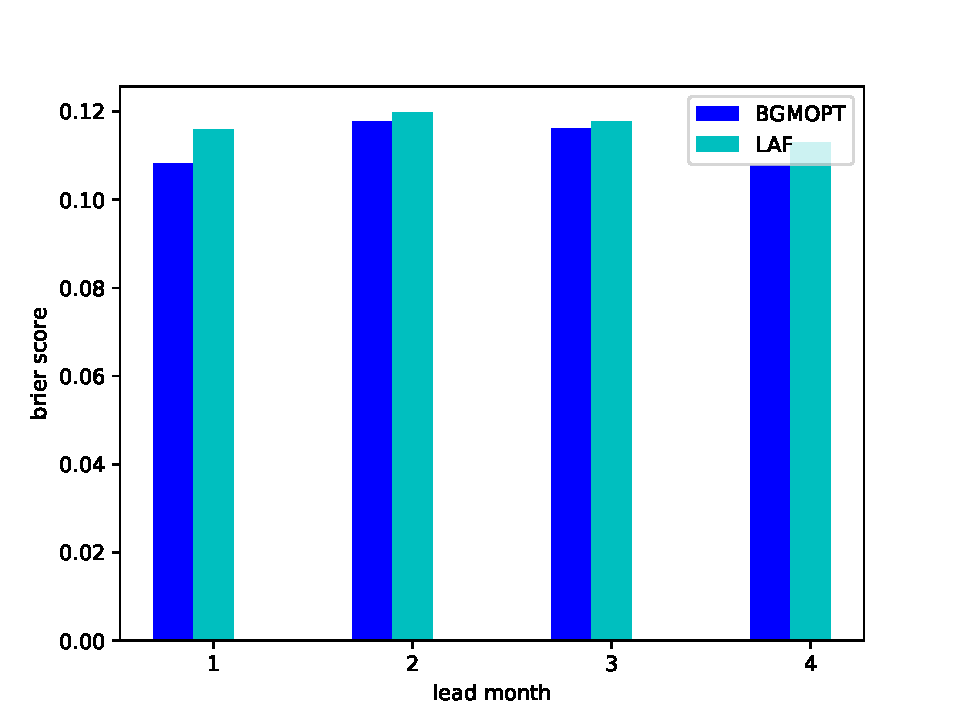
\includegraphics[scale=0.55]{figures/brier.pdf}
  \caption{集合方法关于降水Brier评分结果}
  \label{fig:xfig1}
\end{figure}


\begin{figure}[H] % use float package if you want it here
\label{prectresult}
  \centering
  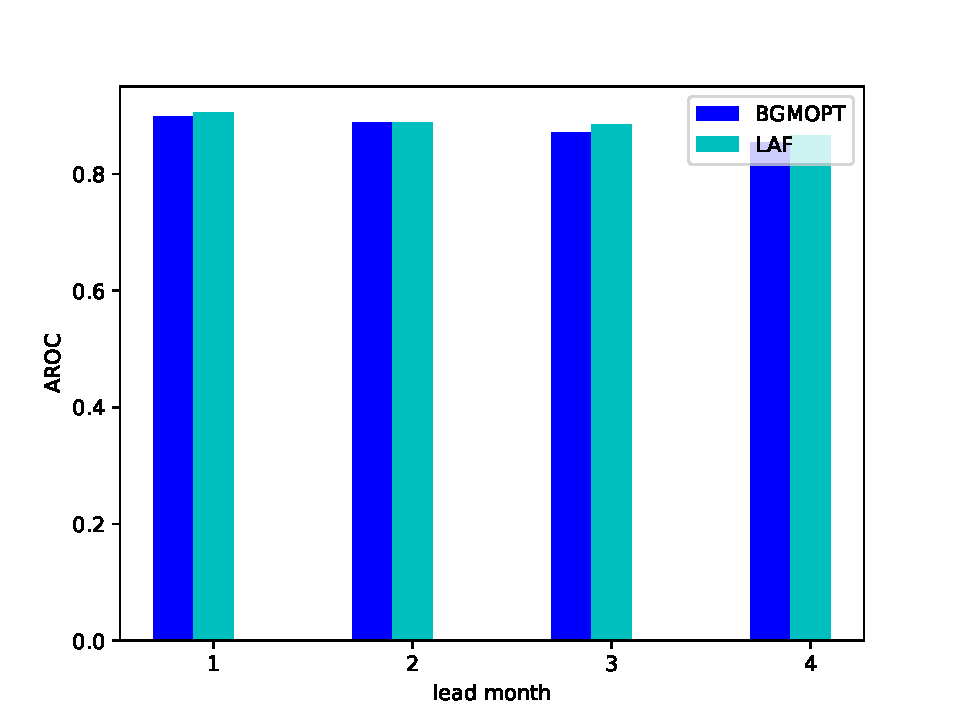
\includegraphics[scale=0.55]{figures/AROC.pdf}
  \caption{集合方法关于降水AROC的评比结果}
  \label{fig:xfig1}
\end{figure}

另外一个经常用来作为集合概率预报的评价的方法是相对操作特征面积ROCA(Relative Operating Characteristics Area)其意义是以假警报率为横坐标,以命中率为纵坐标的ROC曲线下的面积,面积越大则说明预报技巧越高。


\begin{figure}[H] % use float package if you want it here
  \centering
  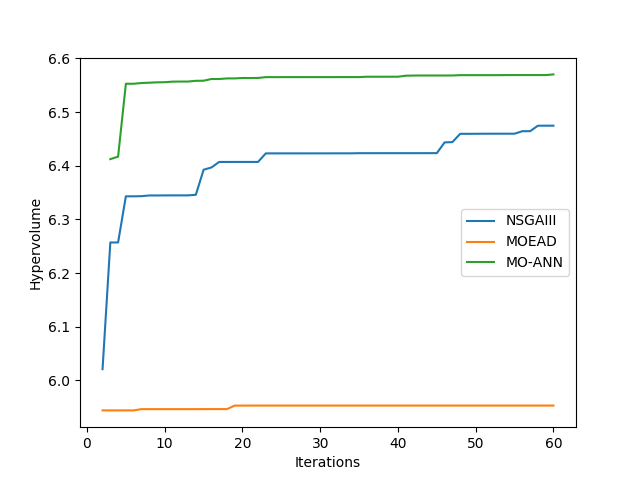
\includegraphics[scale=0.6]{TWPMOnew.png}
  \caption{TWP-ICE单柱大气模型上多目标算法的hypervolume}
  \label{fig:xfig1}
\end{figure} 
\begin{figure}[H] % use float package if you want it here
  \centering
  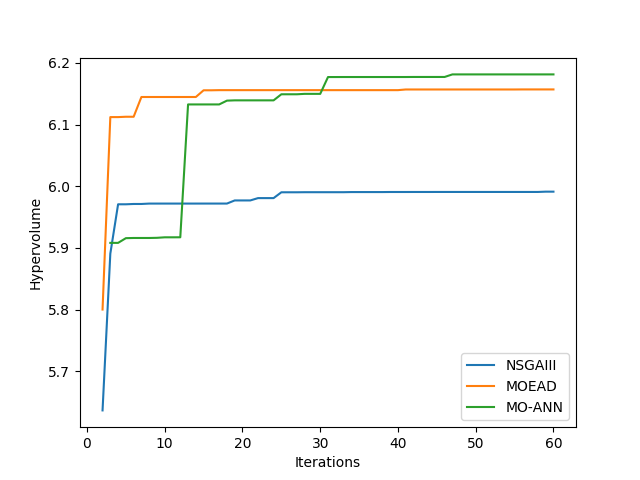
\includegraphics[scale=0.6]{figures/ARW-MO.png}
  \caption{M-PACE单柱大气模型上多目标算法的hypervolume}
  \label{fig:xfig1}
\end{figure} 

\begin{figure}[H] % use float package if you want it here
  \centering
  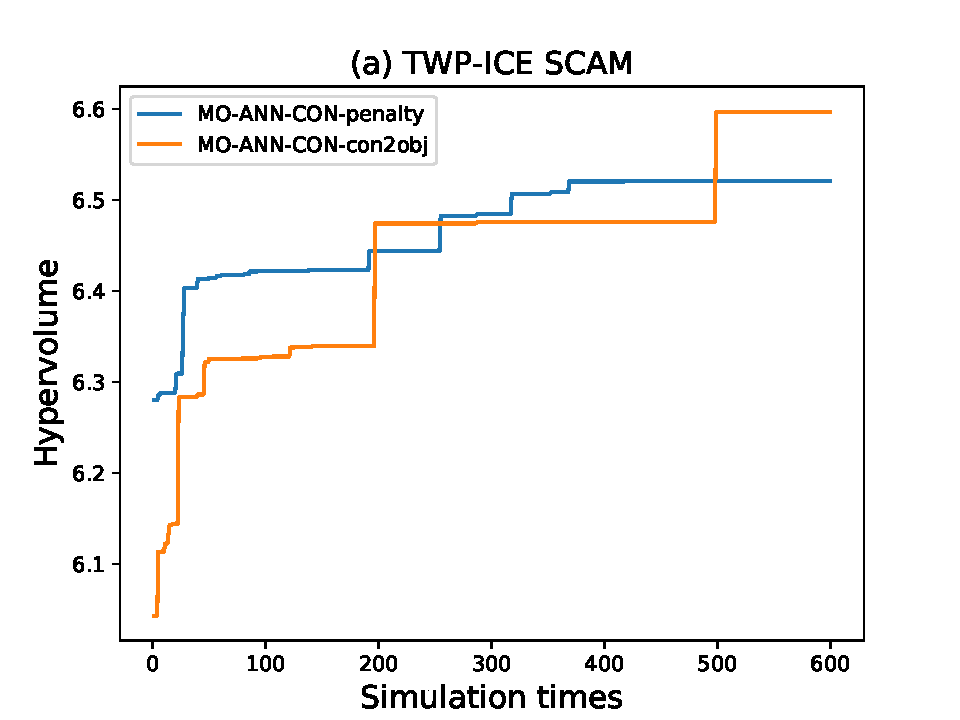
\includegraphics[scale=0.6]{figures/twpconstraint.pdf}
  \caption{TWP-ICE单柱大气模型上有约束多目标算法的hypervolume}
  \label{fig:xfig1}
\end{figure} 
\begin{figure}[H] % use float package if you want it here
  \centering
  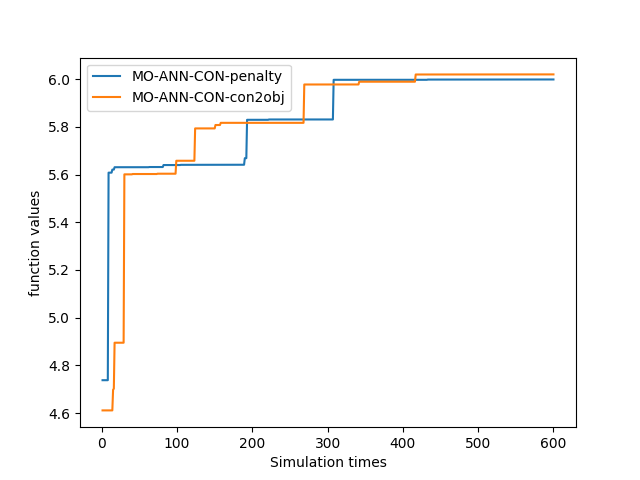
\includegraphics[scale=0.6]{arwconstaint.png}
  \caption{M-PACE单柱大气模型上有约束多目标算法的hypervolume}
  \label{fig:xfig1}
\end{figure}

其典型的例子有基于Kriging模型的EGO(Efficient
Global Optimization)算法~\cite{mohammadi2016kriging}。



\section{面向气候系统模式参数的代理模式优化实现}
\subsection{参数优化准备工作}

参数优化准备工作

1.气候系统模式的移植与验证

2.气候系统模式参数的抽取与验证

\subsection{总体设计}
1.优化问题定义部分。此部分定义问题的输入维度,参数的取值范围,所需要优化的问题。对于气候系统模式的来说,需要优化的是针对某一个评价标准的模式性能表现。这里需要自动化的参数匹配,模式运行和结果评估。如果是多目标优化问题需要利用Hypervolume等指标综合评价非支配解的优劣。

2.代理模式的建立部分。获取参数值与其对应的气候系统模式评价结果样本时需要将样本用来训练代理模式。此模块有MLP的具体实现过程,MLP的总层数以及每一层的隐元个数,激活函数和学习率等超参数的设置。

(1)模型的建立
(2)模型的训练与测试
(2)超参的调优
(3)模型的预测

3.优化算法的优化策略部分。此部分主要是各个代理模式优化算法的最优样本选择策略。在单目标、多目标、有约束优化的实现过程中有些细节上的调整。

4.优化总流程的调度。此部分将面向气候系统模式参数优化的每一个流程串联在一起,包括从一开始的拉丁超立方采样到代理模式的训练再到新的采样点的选取等。
(1)采样
(2)
(2)初始代理模型拟合
(3)新采样点的获取
(4)新采样点的评估

本文中所使用的多层感知机学习率为0.01,隐含层为2,每层隐元数为200,激活函数分别都为sigmoid,输出层的激活函数为Relu,输入层神经元的个数为所需优化参数的维度,输出层神经元的个数为优化目标的个数。在这样一个基础的多层感知机上利用当前所有样本,通过反向传播算法更新神经网络的权重,使其能够很好的拟合当前所有样本。

\begin{figure}[H] % use float package if you want it here
  \centering
  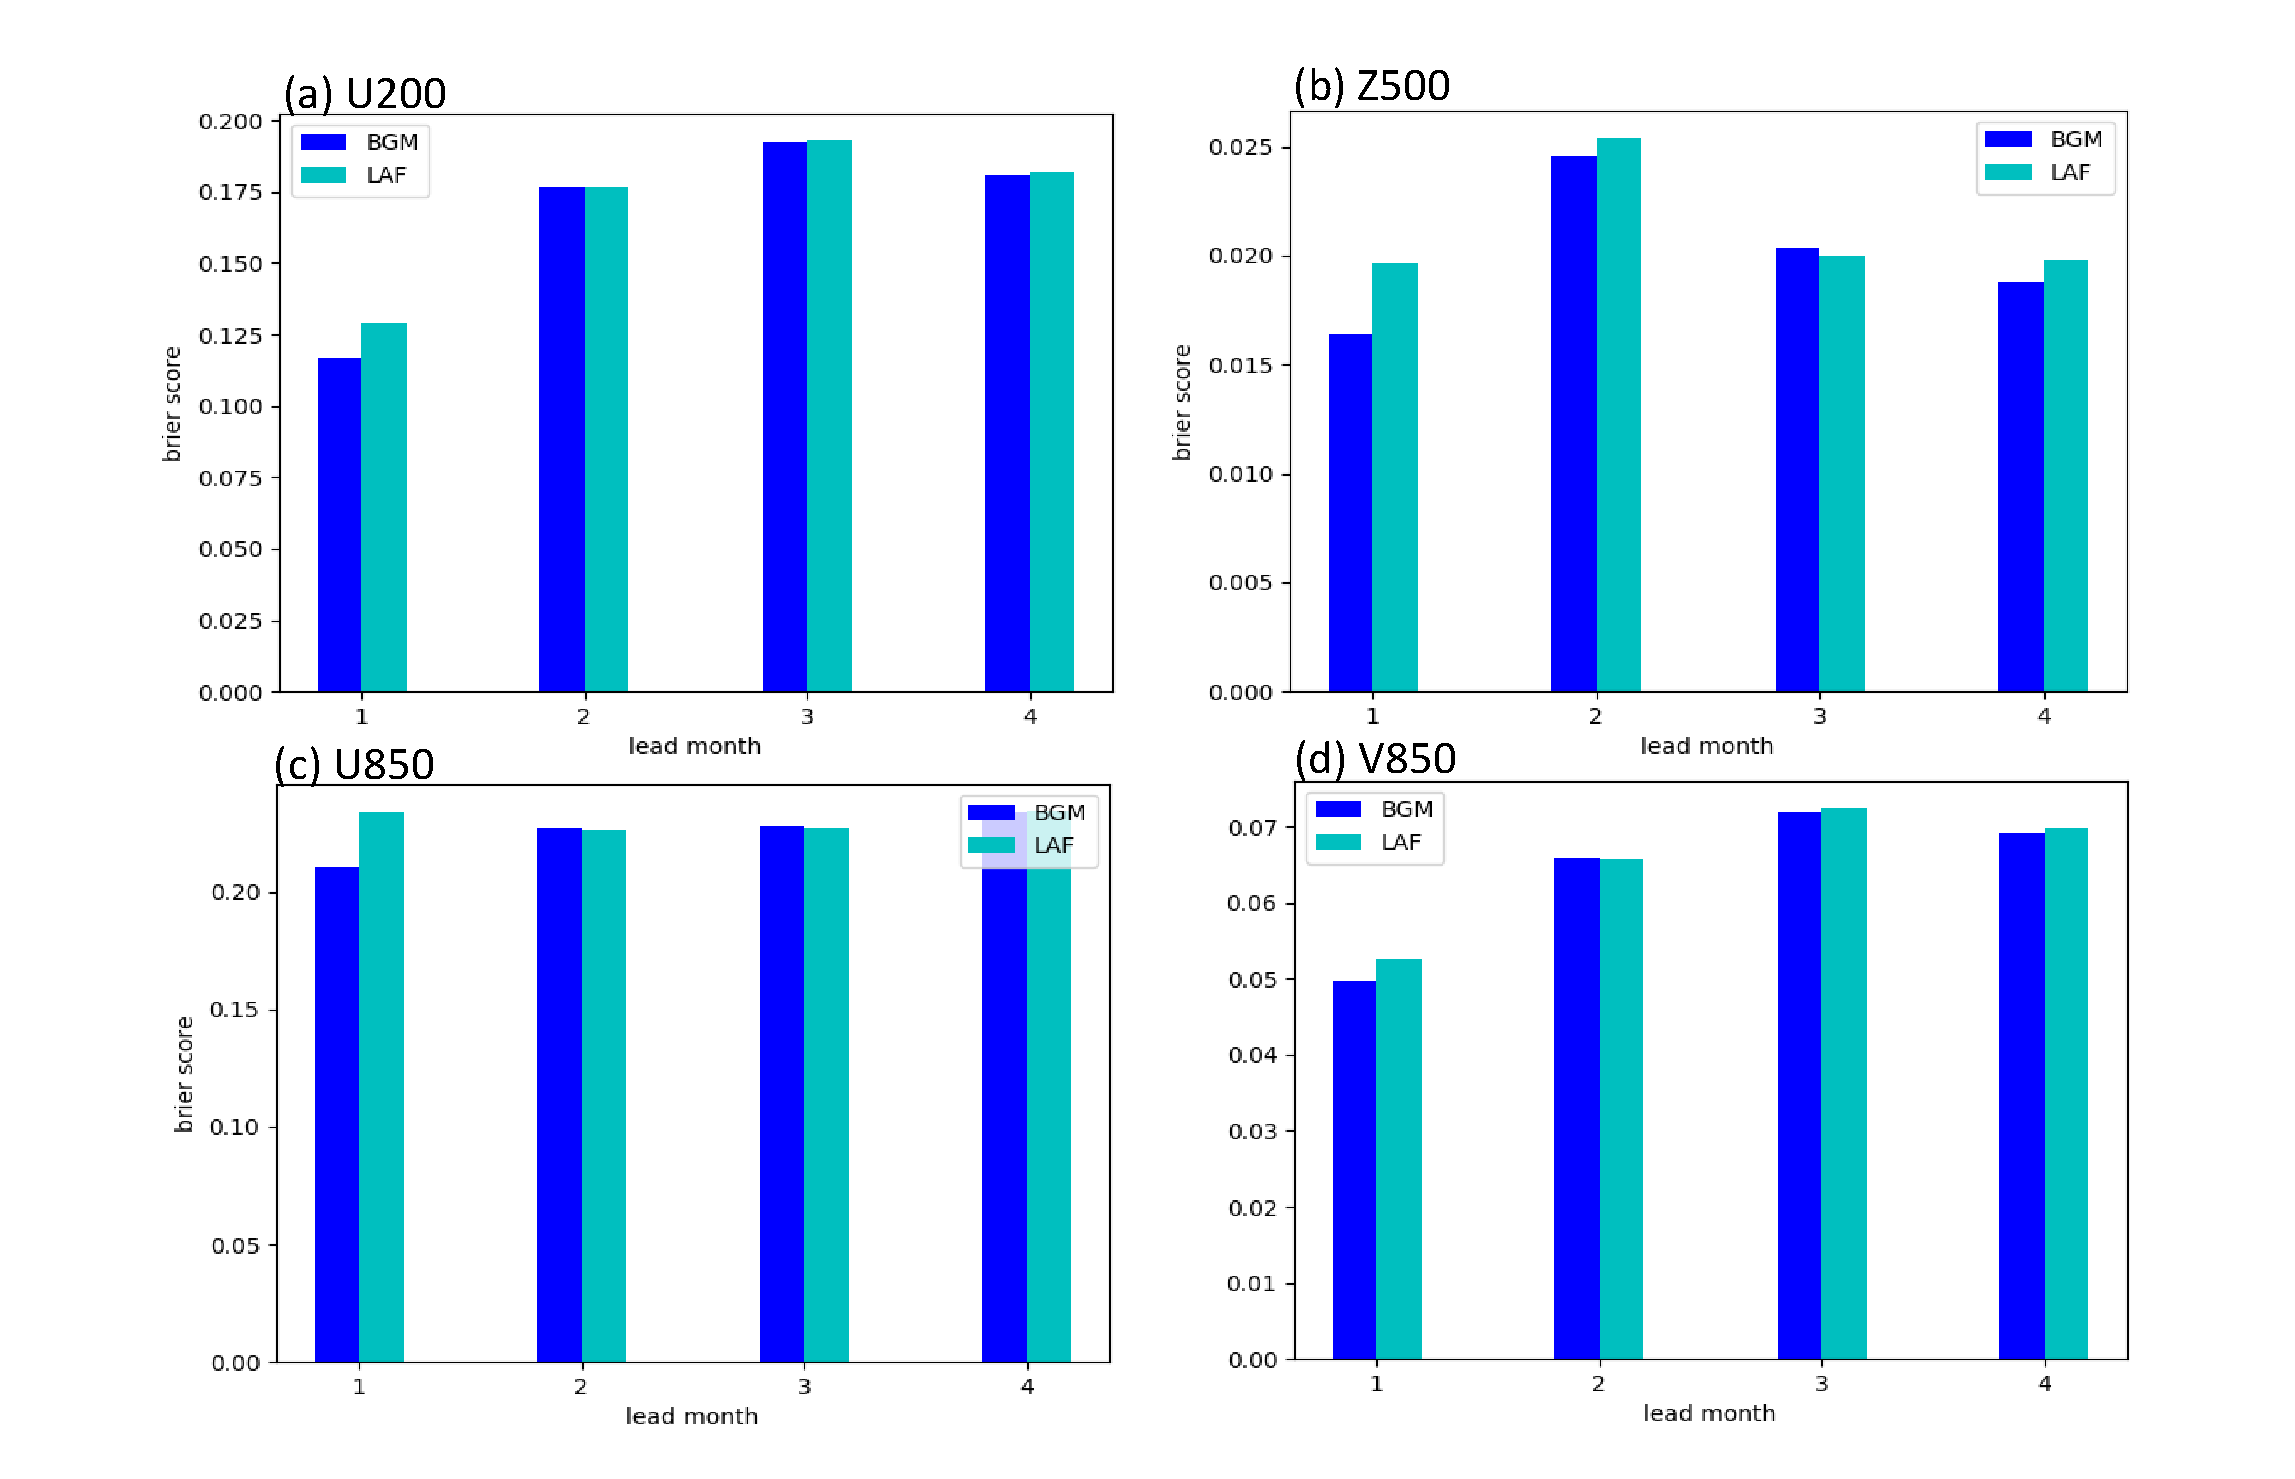
\includegraphics[scale=0.45,trim=60 10 20 10,clip]{figures/allBrier.pdf}
  \caption{U200,Z500,U850,V850全球平均BS评分}
  \label{fig:BS}
\end{figure}




\begin{figure}[H] % use float package if you want it here
  \centering
  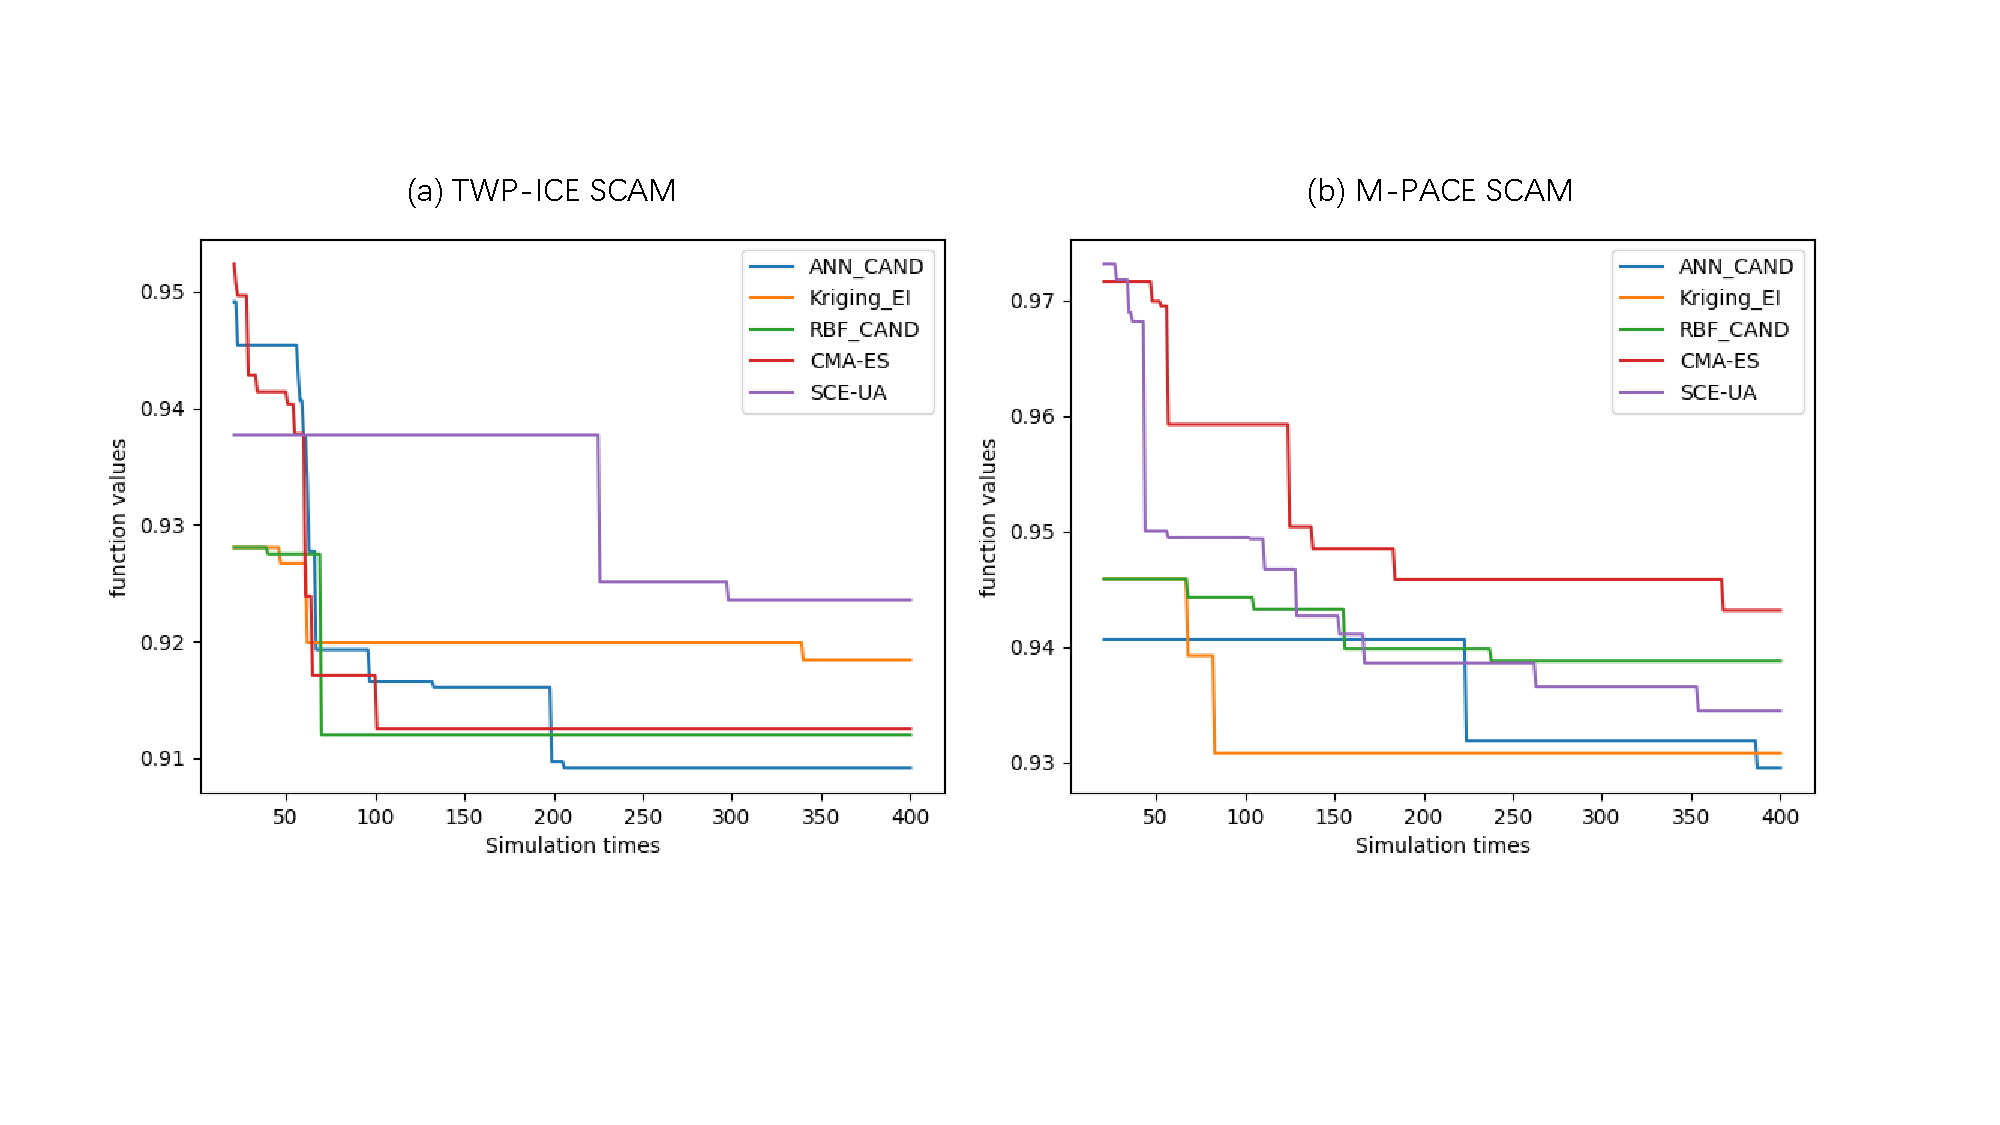
\includegraphics[scale=0.5,trim=10 100 10 85,clip]{figures/soallscam.pdf}
  \caption{单目标优化算法在TWP-ICE和M-PACE单柱大气模式上的优化结果}
  \label{fig:soscam}
\end{figure}

\begin{figure}[H] % use float package if you want it here
  \centering
  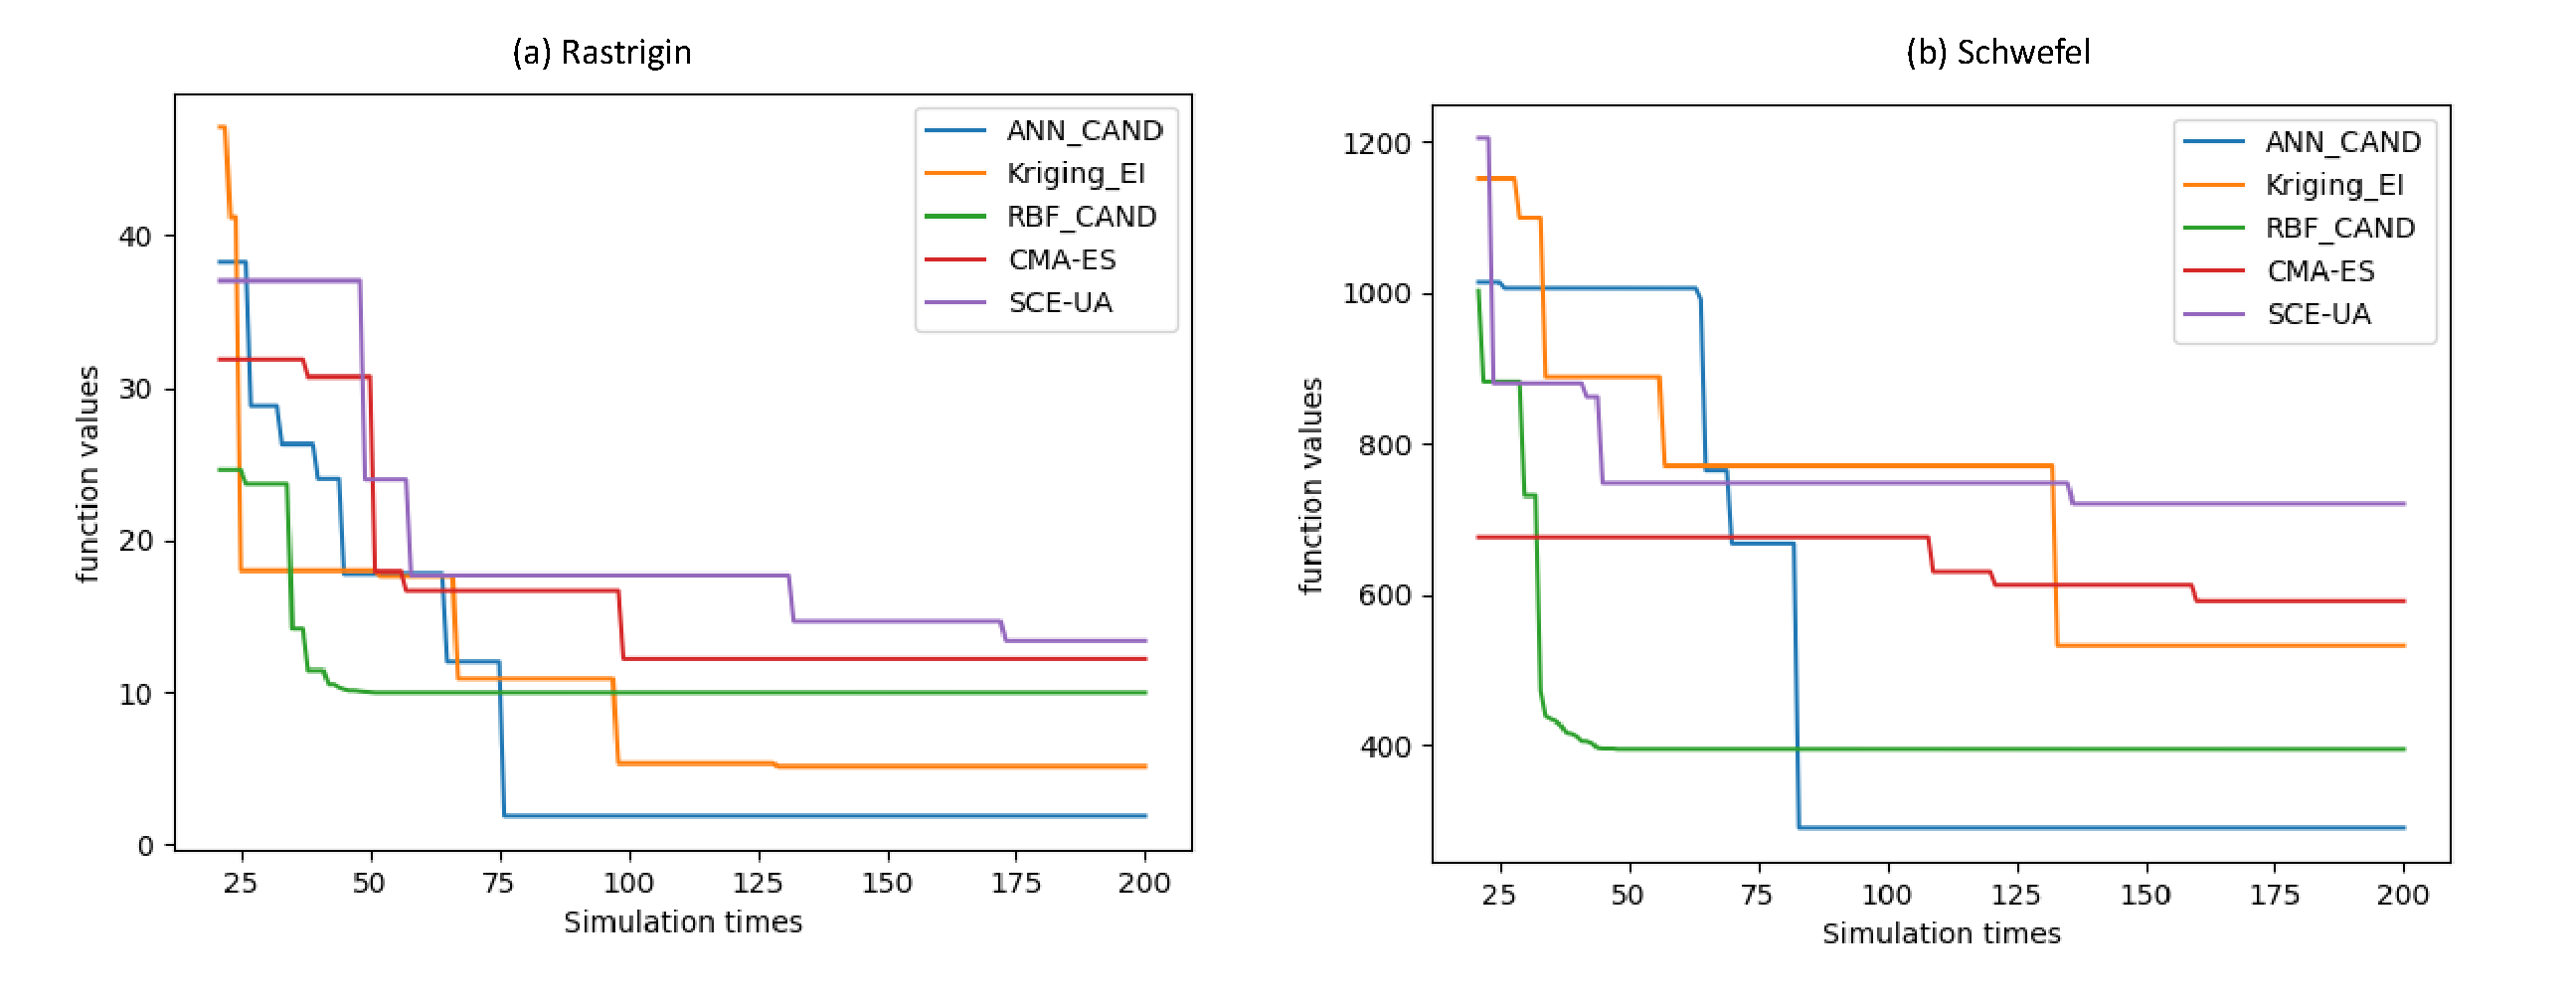
\includegraphics[scale=0.35,trim=0 10 10 10,clip]{figures/SOallfuction.pdf}
  \caption{单目标优化算法在Rastrigin和Schwefel函数上的优化结果}
  \label{fig:sofuction}
\end{figure}










\chapter{气候系统模式不确定参数优化方法设计}
\label{tu:tune}
\section{气候系统模式不确定参数优化问题}

上一章描述了气候系统模式中存在大量的不确定参数,这些参数对气候系统模式的模拟性能有很大的影响,进而影响了预测的准确率。优化算法是一种量化不确定性,校准不确定参数的有效方法。接下来将叙述在气候系统模式不断发展过程中遇到的各种不确定参数优化问题。

气候系统模式中存在一些重要的单一变量,比如降水,它对深对流,云物理等参数化方案中的不确定参数非常敏感。在单一的降水预报时为了提高预测能力需要针对降水对不确定参数进行校准。Yang B等人在中尺度天气预报模型WRF(Weather Research and Forecasting Model)中利用MVFSA(multiple very fast simulated annealing)方法对深对流中的不确定性参数做了校准~\cite{yang2015calibration}。

衡量一个气候系统模式整体性能的时候,通常会将多个变量综合在一起,形成一个较为全面的性能指标,在这个性能指标下优化模型的不确定参数。张涛等人将GAMIL( Grid-point Atmospheric Model of IAP LASG)大气模式中受到关注最多的变量综合成一个用来衡量模式平均态的综合性能指标,并利用改进的单纯形下山方法对GAMIL大气模式中对流和云等参数化方案中的不确定参数进行了调整~\cite{zhang2015automatic}。

上述问题都可以用单目标优化问题来描述,但是在气候系统模式参数优化中多目标优化也不可或缺。例如当模式预报的目标有两个以上,比如降水、温度和湿度等对预测十分重要的变量都需要尽可能得到优化,如果使用上述将多个变量综合成一个目标的方法,则有可能会出现整体的性能得到提升,但其中某个关键变量却变得很差的情况。此时需要利用多目标优化来对不确定参数进行校准。另外在气候系统模式中有很多非常重要的气候现象,例如热带大气季节内震荡(MJO)、东亚季风(EASM)、厄尔尼诺/南方涛动(El Niño–Southern Oscillation)等,这些分别是属于不同物理意义的气候现象,在气候系统模式中都十分重要,如果要找到使这些气候现象模拟结果都变好的优化参数也同样需要使用多目标优化方法。多目标优化在气候系统模式的参数优化中非常重要,但是目前它的应用却不是很多。究其原因还是因为气候系统模式本身运算代价高,此时再对其进行多目标优化更增添了问题的复杂性,且计算量难以接受。

从单目标到多目标优化,气候系统模式的优化方法思路逐渐清晰,但是这些算法都完全将气候系统模式当成一个黑盒问题。不考虑其内部的机理,而这样的优化方法很有可能导致气候系统模式中的一些重要的物理约束条件被打破。例如耦合模式模式顶的辐射平衡,其物理意义是模式进来的太阳的短波辐射和出去的长波辐射总量是一样的,只有这个条件得到满足,耦合模式的能量才能守恒,才能长期稳定的运行。Hourdin等曾提出,耦合模式大气顶的辐射偏差超过1W/m$^2$将会导致地表温度改变0.5-1.5K以上~\cite{hourdin2017art}。Wild等也指出辐射偏差在GCMs(General Circulation Models)模型中可能会影响气候敏感性,这将会导致对未来气候预测的扭曲~\cite{wild2008short}。

综上所述,在气候系统模式中急需高效、收敛快的单目标和多目标优化算法。与此同时要密切关注所优化的问题中是否有物理条件约束,如果有,则需要提出针对性的有约束优化算法。

本章接下来先将详细说明单目标、多目标、有约束代理模式优化方法是如何设计的,然后将新设计方法与已有算法在复杂的数学函数和单柱模式上进行了测试和对比以验证新提出算法的有效性,最后叙述了如何将本文提出的各类基于多层感知机神经网络的代理模式优化方法进行整合以适应所有气候系统模式的物理参数优化问题。

%\section{从单目标到多目标的气候系统模式参数优化方法}

\section{气候系统模式不确定参数的单目标优化方法}
\subsection{单目标优化方法设计}
目前可以用于气候系统模式参数优化问题的单目标优化算法主要有以下几类。一是传统的局部优化算法,例如单纯型下山、鲍威尔法(powell)等,这一类算法容易过早陷入局部最优,因此本文没有对其进行测试。

第二种方法是智能进化算法,它是目前最重要的单目标优化方法类型之一,也是在气候系统模式中被广泛应用的方法。其思想是模拟自然界中生物种群进化的过程,每一代种群中,表现最好的个体将有更大可能保留他们自己的基因到下一代,如此循环迭代,直到满足优化的条件。常用的进化算法有模拟退火(SA)、遗传算法(GA)、差分进化(DE)、粒子群优化算法(PSO)、协方差自适应调整进化策略(CMA-ES)和单纯多边形进
化算法(SCE-UA)等。其中CMA-ES和SCE-UA因为其良好的收敛性和全局性被广泛应用于多个领域。例如CMA-ES被应用于机器人以及强化学习中~\cite{wang2010optimizing,salimans2017evolution},SCE-UA被应用于水文和气象领域的参数优化~\cite{duan1993shuffled,江净超2017知识驱动下的水文模型参数智能化设置方法,ma2006application}。

第三种是基于模型的时序优化方法,这一类方法通常被称为代理模式优化,它的思路是利用当前所有样本构建一个统计回归模型称为代理模式,然后利用代理模式去估计下一个更优参数的位置。将此处得到的最优参数代入真实模式中运行,获得新的真实的采样点,将此采样点加入原有样本,一起构建新的代理模式。如此反复迭代,直到新估计的采样点满足优化条件。代理模式优化在对高计算代价的问题上应用广泛。其算法思想如算法1所示。

\floatname{algorithm}{算法}
\renewcommand{\algorithmicrequire}{\textbf{输入:}}
\renewcommand{\algorithmicensure}{\textbf{输出:}}
\begin{algorithm}
        \caption{基于代理模式的优化方法思路}
        \begin{algorithmic}[1] %每行显示行号
            \Require 原模型$F$, 待调参数$X$, 采集函数$AF$, 代理模型$M$
            \Ensure 优化参数
            \State $S \gets InitSamples( F, X )$
            \For{$i = 0 \to T$}
                \State $p( y| x, S ) \gets FitModel(M, S)$
                \State $xnew_i \gets argmax_{x\in X}AF(x,p(y|x,S))$
                \State $ynew_i \gets F(x_i)$  //expensive step
                \State $S \gets S \cup (xnew_i,ynew_i)$
            \EndFor
        \end{algorithmic}
\end{algorithm}

其中$F$为真实的复杂的代价高的问题,例如本文这里的气候系统模式,$X$为待调整参数,$AF$为采集函数,即为如何选取下一个新的采样点的策略。代理模型$M$是作为一个低代价的对于原问题的回归模型。

常用的代理模式的模型选择有克里金法(Kriging),径向基函数(RBF)和多元⾃适应回归样条(MARS)等~\cite{xu2018parameter}。其中Kriging和RBF应用最为广泛。采集函数有随机策略,EI( Excepted improvement)策略,构建最优点附近的随机扰动候选样本集策略(本文中称之为CAND)等。下文将分别简单介绍常用代理模型Kriging和RBF以及采集函数EI和CAND。

1.克里金(Kriging)方法:它是一种多项式和随机过程叠加的回归方法,最早是由南非的地质学家Krige在1951年提出来的,一开始主要用于地质领域。其一般形式如下:
\begin{equation}
\label{equ:Rasfuc}
Y ( \mathbf { x } ) = \mu + \varepsilon ( \mathbf { x } )
\end{equation}
其中$\mu$为多项式项,$\varepsilon ( \mathbf { x } )$是随机过程项,对于简单的以高斯过程作为随机项的普通Kriging模型来说,$\mu$是高斯过程的平均值,$\varepsilon ( \mathbf { x } )$是高斯过程的误差项,通常$\varepsilon ( \mathbf { x } )$是一个均值为0,方差为$\sigma ^ { 2 }$的正太分布。
%根据此空间相关性构建预测模型误差项,
%Kriging模型预测公式如下所示:
%\begin{equation}
%\hat { y } ( \mathbf { x } ) = \hat { \mu } + \mathbf { I } ^ { \mathrm { T %} } \mathbf { C } ^ { - 1 } ( \mathbf { y } - \mathbf { 1 } \hat { \mu } )    
%\end{equation}
%\begin{equation}
%s ^ { 2 } ( \mathbf { x } ) = \hat { \sigma } ^ { 2 } \left[ 1 - %\mathbf { c } ^ { \mathrm { T } } \mathbf { C } ^ { - 1 } \mathbf %{ c } + \frac { \left( 1 - \mathbf { 1 } ^ { \mathrm { T } } %\mathbf { C } ^ { - 1 } \mathbf { c } \right) ^ { 2 } } { \mathbf %{ 1 } ^ { \mathrm { T } } \mathbf { C } ^ { - 1 } \mathbf { 1 } } %\right]    
%\end{equation}

2.径向基函数(RBF):RBF中的径向函数是一种以待测点和样本点之间的欧式距离为自变量的函数,径向基函数是以径向函数为基函数线性叠加而成。它构造模型的公式如下所示,其主要思想是利用径向基函数和全局倾向函数共同来构建一个插值回归模型。它在图像处理,函数逼近等多个领域内得到广泛的应用。
\begin{equation}
y = \sum _ { i } ^ { n } \omega _ { i } \dot \varphi \left( \left\| x - x _ { i } \right\| _ { 2 } \right) + g ( x )
\end{equation}
其中$\varphi$为径向基函数,$g (x)$由$\varphi$所决定。

采集函数为估计下一个最佳采样点的方法,常用的方法有随机策略,EI( Excepted improvement),构建当前最优点附近的随机扰动候选样本库策略(本文中称之为CAND)等。EI策略就被用在EGO(Efficient Global Optimization)算法中,CAND策略也经常被用于构建代理模式。接下来分别介绍这两种策略。

1. EI策略:它的思想主要是通过最大化期望函数$I(x)$,即找出使得$I(X)$最大化的$X$取值。
\begin{equation}
I ( \mathbf { x } ) = \max \left( f _ { \min } - Y ( \mathbf { x } ) , 0 \right)   
\end{equation}
其中$ f _ { \min }$为当前所有采样点中$y$的最小值。即当前获得的最佳的真实模型上的优化结果,$Y(X)$为代理模型预测的采样点$X$处的$Y$值。

2. CAND策略:它的思想是通过找出当前使得目标Y结果最好的输入X,然后在X附近进行扰动,获取一系列扰动点,将这些扰动点分别在已有的代理模式上进行评测,评测结果最优的扰动点即为真实模式上的下一个采样点。

目前最常用的两种代理模式优化方法为基于Kriging模型和EI采集函数的EGO算法~\cite{mohammadi2016kriging},以及基于RBF模型和CAND采集函数SRBF~\cite{regis2007stochastic}算法。这两种方法被广泛应用于多个领域的建模及参数优化工作。
%最优样本估计策略是EI方法。其算法流程图如下所示:

%RBFSBO算法是由于2012年提出的,其思路是利用

%本文新提出算法1的流程如下
%\begin{figure}[H] % use float package if you want it here
%  \centering
%  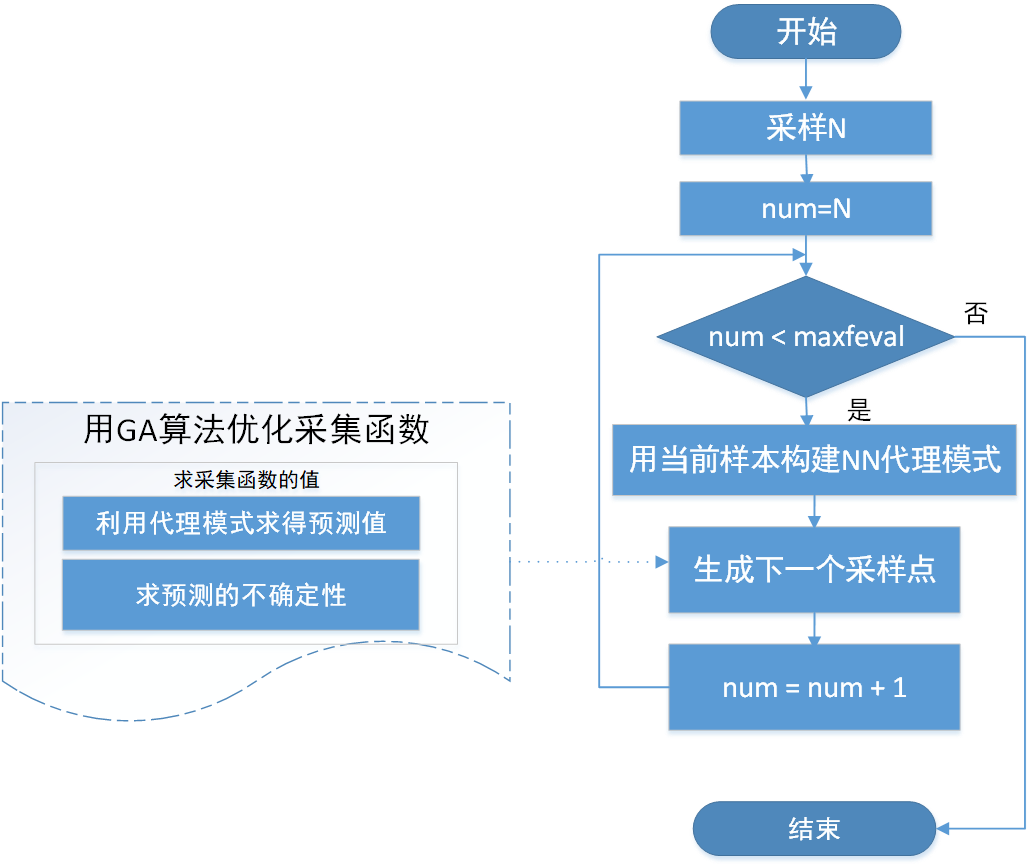
\includegraphics[scale=0.6]{ANN_Kriging流程图.png}
%  \caption{ANNKriging流程图}
%  \label{fig:xfig1}
%\end{figure}
综合前文所述,当前最常用的单目标算法在处理复杂气候系统模式参数优化中面临的主要问题有以下几点:

1.进化算法的种群更新策略慢,优化迭代步数多。在复杂的气候系统模式上进行参数优化是一件高代价的事情,如果优化算法迭代步数多则意味着更多次的模式运行,更多的计算资源被消耗。

2.基于传统代理模式的优化方法代理精度不足。在传统的代理模式优化中,代理模型的选择通常为统计回归方法,这些方法对复杂多峰的气候系统模式的代理精度不足,这将会导致基于代理模式的最优参数估计不够精准,进一步影响优化算法的精度。

面对以上问题,本节设计了基于多层感知机代理模式的优化方法ANN\_CAND。它的主要思想是:(1)利用传统代理模式优化的快速更新策略,ANN\_CAND在初始采样后每一个最优采样点的选取都需要更新优化策略,以期望实现快速的算法收敛过程;(2)利用神经网络的强回归能力弥补现有代理模型在气候系统模式上的代理精度不足的问题,以实现更高的优化精度。

本文中提出的单目标ANN\_CAND优化方法如算法2所示。重要步骤的详细解释如下。

1.初始采样。初始采样有两个重要的目的。其一是为了初步探索参数空间使得优化算法对参数空间有一个基本的了解。其二是为了初始化代理模式。如引言中所介绍,采样方法有很多,这里选择的拉丁超立方采样,它的思想是在参数空间中分层随机抽样。因为有了分层的策略,采样在参数空间中较为全面,能够将优化算法建立在一个良好的基础上。

2.构建基于多层感知机的代理模式。根据气候系统模式的参数到性能的复杂特性,此算法中选择的建模方法是具有更强非线性表达能力的多层感知机神经网络。它是一种前向的人工神经网络(ANN),可以看成一组输入向量到一组输出向量的映射。它由多个节点层所构成,层与层之间全连接,且除了输入层之外,其他的节点层都是带有非线性激活函数的神经元。多层感知机神经网络在非线性回归上十分受欢迎,研究表明多层感知机是通用的函数逼近器,甚至适合非光滑和分段连续回归问题,且其相对于传统的机器学习算法而言,它具有更高的拟合精度~\cite{selmic2002neural}。

3.通过采集函数获取下一个采样点。采集函数为改进后的CAND策略。其主要思想是构建两组候选采样点集合,第一组为在当前最优点处的随机扰动,第二组为在全参数空间中的随机扰动。然后利用两种评价相结合的方法对所有候选集采样点进行评价。第一种评价方法是利用代理模式对采样点进行估计,估计结果好的,被选取的机会大,第二种评价方式是根据候选集中的采样点与当前已有采样点的距离来衡量的,距离越近,估计的结果越准确。另外为了平衡这两个评价策略,引入了一个权重参数weight,weight的值越大,对当前代理模式预测的信任度越高。两组候选集独立选取,平衡了优化过程中的探索与利用。两种评价方式的综合也更加全面地估计了一个候选采样点可能的结果。

4.在真实的模型上评估新采样点的结果。最后将此CAND策略选出的最优样本点带入真实模型中运行,得到真实的采样结果。这一步在复杂函数中为函数值的计算,在气候系统模式中则为一次模型运行和评估的过程。

5.将新采样点加入样本集,重新拟合代理模式。将这一对结果加入已有样本库,重新构建模型。依此重复,直到算法收敛或者是达到规定的迭代步数。

\floatname{algorithm}{算法}
\renewcommand{\algorithmicrequire}{\textbf{输入:}}
\renewcommand{\algorithmicensure}{\textbf{输出:}}
\begin{algorithm}
        \caption{ANN\_CAND单目标优化方法}
        \begin{algorithmic}[1] %每行显示行号
            \Require 原模型$F$, 待调参数$X$, MLP神经网络$M$,利用率$weight$
            \Ensure 优化参数
            \State $S \gets InitSamples( F, X )$
            \For{$i = 0 \to T$}
                \State $FitMLP(M, S)$
                \State $xnew_i \gets \Call {CandMethod}{X,Y,MLP,weight}$
                \State // 将最优估计样本带入真实问题中求解
                \State $ynew_i \gets F(x_i)$
                \State // 将新样本加入已有样本库
                \State $S \gets S \cup (xnew_i,ynew_i)$
            \EndFor
            \Function{CandMethod}{$X,Y,MLP,weight$}
              \State // 获取当前最优结果对应的$X$
              \State $index \gets argmin(Y)$
              \State $current\_bestX \gets X(index)$ 
              \State // CandPoinSet作为下一个采样点的候选集,分为两组,第一组为在当前最优点$X$附近的扰动,另一组为在$X$全空间内的随机扰动
              \State $CandPointSet \gets [RandPerturbatio(current\_bestX),Xrandom]$
              \State // 利用当前训练好的$MLP$模型预测所有的采样候选集
              \State $CandValueSet \gets MLP.predict(CandPointSet)$
              \State // 计算候选集中的点与当前X的距离
              \State $dis\_metrics(CandPointSet) \gets distance(CandPointSet,X)$
              \State // 关于候选集$X$的评价策略分为两部分,第一部分为$MLP$模型对其的预测值,另外一个部分为其与当前采样点的距离
              \State $metrics \gets weight * CandValueSet + (1-weight) * dis\_metrics(CandPointSet)$
              \State  // 选取上述metrics评价最小的点作为下一个最优采样点
              \State $indict \gets argmin(metrics)$
              \State $CandPoint \gets CandPointSet(indict)$
            \EndFunction
        \end{algorithmic}
\end{algorithm}

%\begin{figure}[H] % use float package if you want it here
%  \centering
%  \includegraphics[scale=0.6]{all_SCAM.png}
%  \caption{SCAM在二维参数的变化下导致的性能变化}
%  \label{fig:xfig1}
%\end{figure} 


%对比传统算法,新算法在理论上有以下几点优势。
\subsection{单目标优化方法性能评估}
 为了验证上述单目标优化方法的有效性,分别在复杂数学函数和单柱大气模式(SCAM)上对各类单目标算法进行了测试。因为在真实的气候系统模式中希望以尽可能少的模式运行次数来确定最优参数,以下评比所遵循的规定是对数学函数的计算次数在200次以内,在单柱大气模式上的模拟次数在400次以内,查看在此范围内各类优化算法的表现情况。其中Kriging\_EI是以Kriging为建模模型,以EI为采集函数的代理模式优化方法。RBF\_CAND是以RBF为建模模型,本文中的CAND方法为采集函数。
 
   1.在复杂函数上的测试
   
     为了尽可能模拟复杂的气候系统模式的特点,在这里选择的测试函数是有多个局部最优解,非线性变化较强的Rastrigin和Schwefel~\cite{pohlheim2007examples}函数。Rastrigin公式表达如下所示,
\begin{equation}
\label{equ:Rasfuc}
f ( \mathbf { x } ) = A n + \sum _ { i = 1 } ^ { n } \left[ x _ { i } ^ { 2 } - A \cos \left( 2 \pi x _ { i } \right) \right]
\end{equation}     
     其中$A = 10$,$x _ { i } \in [ - 5.12,5.12 ]$,它在二维参数情况下的函数值变化如图~\ref{fig:sofunctionspace} (a)所示。
Schwefel函数表达式如下:
\begin{equation}
\label{equ:Rasfuc}
     f ( \mathbf { x } ) = 418.9829 d - \sum _ { i = 1 } ^ { d } x _ { i } \sin \left( \sqrt { \left| x _ { i } \right| } \right)
\end{equation} 
其中$x _ { i } \in [ - 512,512 ]$,它在二维参数情况下的函数值变化如图~\ref{fig:sofunctionspace} (b)所示。

\begin{figure}[H] % use float package if you want it here
  \centering
  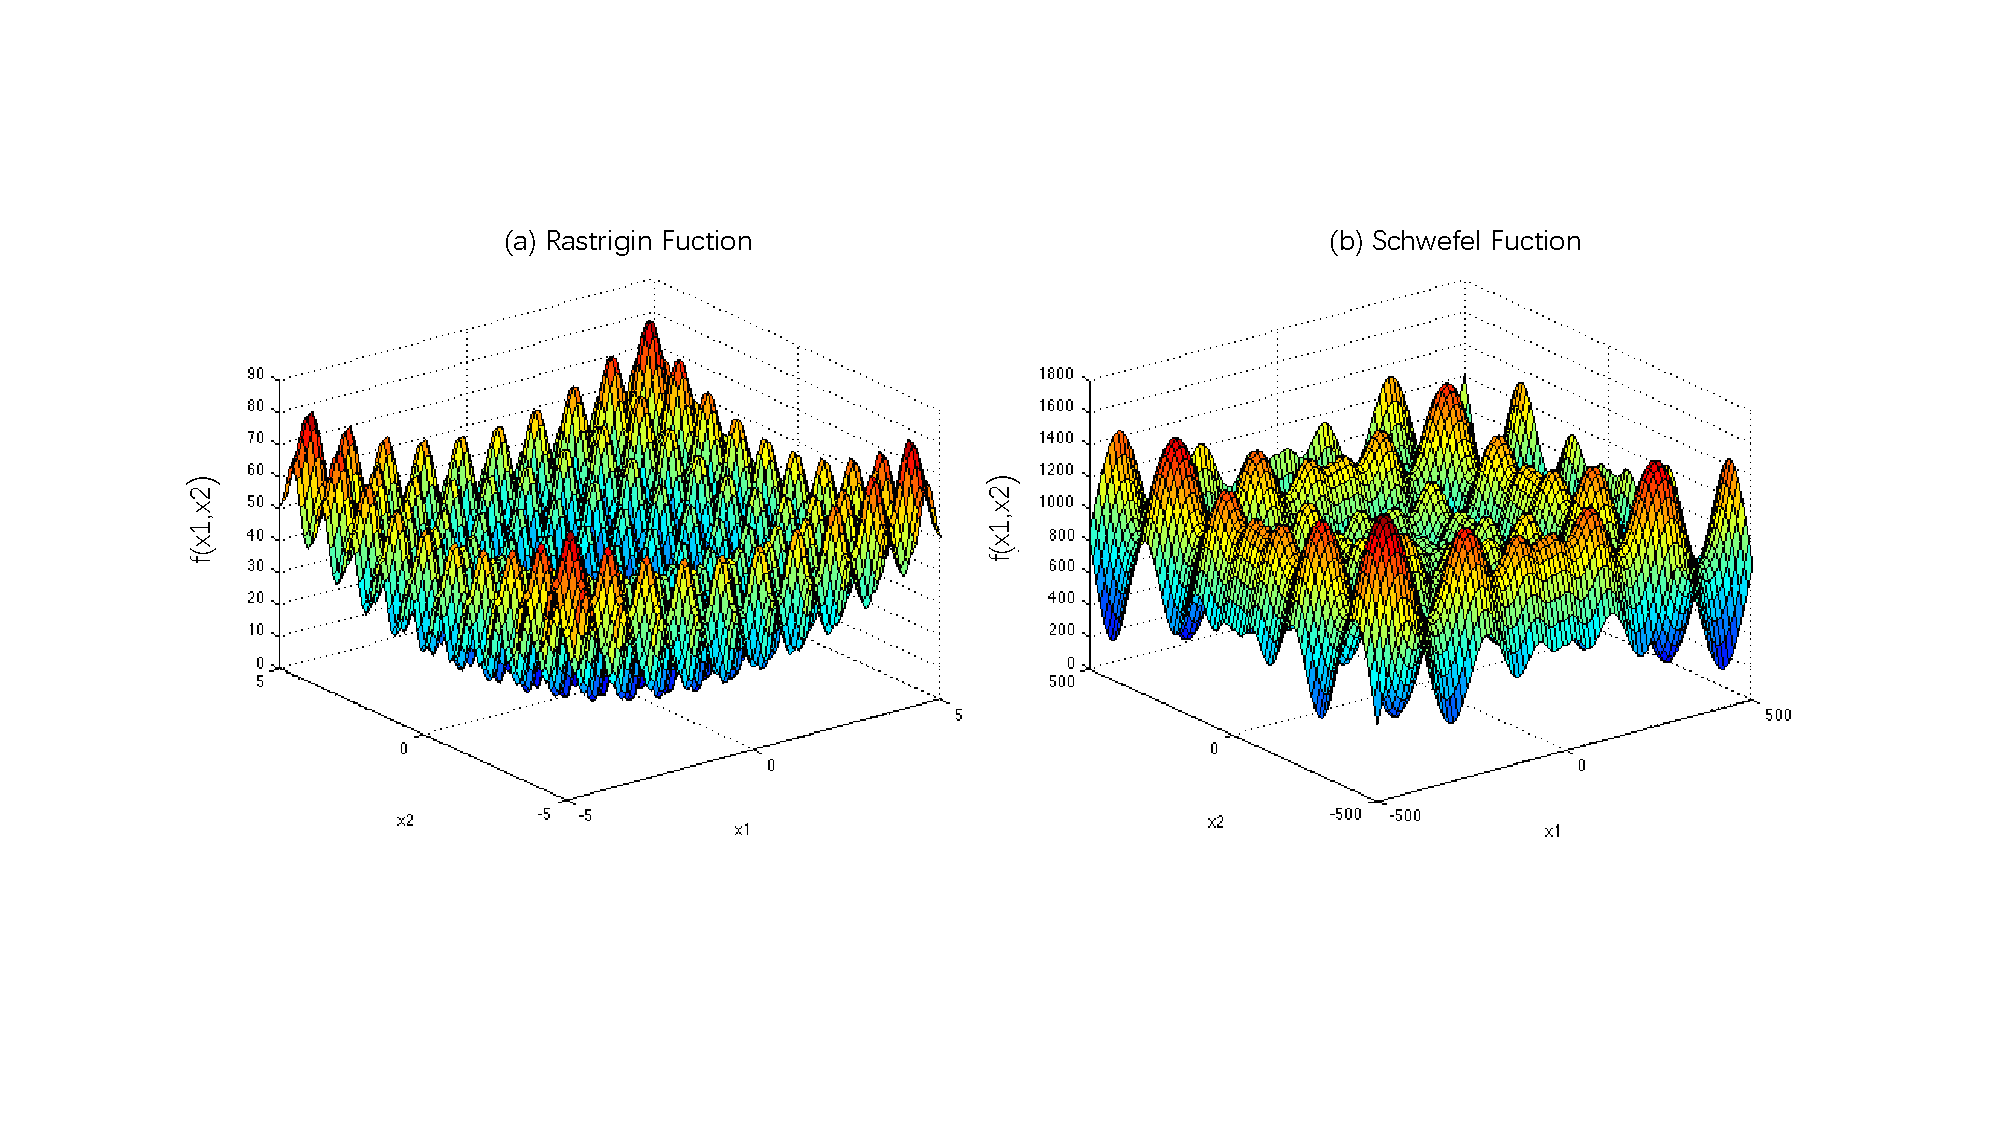
\includegraphics[scale=0.5,trim=10 90 10 100,clip]{figures/fuctionspace.pdf}
  \caption{Rastrigin和Schwefel函数二维空间图(摘自文献~\cite{optfun1,optfun2})}
  \label{fig:sofunctionspace}
\end{figure}

 %   为了验证新算法在参数空间为低维和高维的情况下的性能,这里针对Rastrigin有两组实验,实验1的参数维度为4,实验2的参数维度为12。
 这里将新算法和进化算法以及传统的Kriging和RBF等方法进行比较的结果如图~\ref{fig:sofuction}所示。在Rastrigin和Schwefel函数的优化中基于MLP代理模式的优化算法ANN\_CAND表现较好,和Kriging\_EI,RBF\_CAND一样它相对进化算法能够快速获得较好的优化结果。另外由于选用了更加精准的代理回归方法,它相比于Kriging\_EI和RBF\_CAND而言又能进一步在精度上有所提高。
\begin{figure}[H]
\centering
\begin{minipage}[t]{0.48\textwidth}
\centering
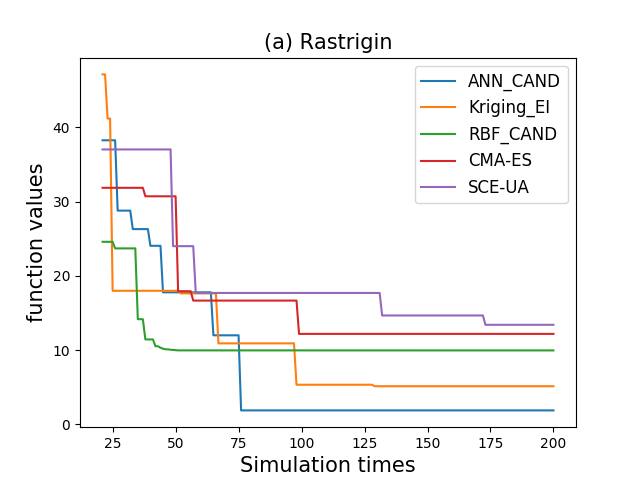
\includegraphics[width=8cm]{figures/all_Ra4.png}
%\caption{ZDT2 hypervolume}
\end{minipage}
\begin{minipage}[t]{0.48\textwidth}
\centering
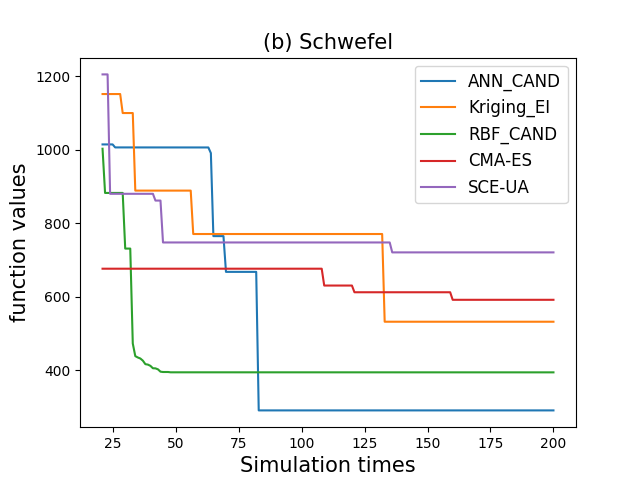
\includegraphics[width=8cm]{figures/all_schw4.png}
%\caption{ZDT2 IGD}
\end{minipage}
\caption{单目标优化算法在Rastrigin和Schwefel函数上的优化结果}
\label{fig:sofuction}
\end{figure}

   2.在单柱大气模式上的测试
   
复杂函数的测试只能证明新算法对于一般复杂的数学问题上的有效性,为了进一步验证其是否能在气候系统模式的不确定性参数调整的实际应用中有较好的表现,本文选择了SCAM( Single Column Atmosphere Model )模式进行测试。SCAM是固定在某个经纬度的单柱大气模式,它是由的特定的边界场和强迫场驱动的,是专门为了研究物理参数化方案而开发的工具,对气候系统模式的发展有重要意义。本文选择的是TWP-ICE~\cite{lin2012twp}和M-PACE~\cite{verlinde2007mixed}实验。TWP-ICE实验的模拟时间是从2006年1月18日至2月13日。M-PACE实验的模拟时间是从2004年10月06日至10月22日。两SCAM个实验性能评价指标是大气模块中最受关注的一些变量,具体的变量选择如表2.1所示。

%%%%table1

%%%%table2
\begin{table}[H]
\centering
\caption{目标变量及其含义}  
\begin{tabular}{ll}
\toprule[1.5pt]
变量名称 & 变量含义 \\  
\hline  
FLUT     & Upwelling longwave flux at top of model   \\
    FSNTOA   & Net solar flux at top of atmosphere   \\
    PRECT    & Total precipitation rate   \\
    Q850     & Specific humidity at 850hPa   \\
\bottomrule[1.5pt]  
\end{tabular}  
\end{table}  
%%%%table3
%\begin{table}[htb]
%\centering
%\caption{相关性分析}  
%\begin{tabular}{llllll}
%\toprule[1.5pt]
%    & FLUT & FSNTOA & PRECT &Q850 &T850 \\  
%\hline  
%FLNT     & 1        & -0.34247 & 0.22897  & 0.03541  & %0.29663 \\
%    FSNT     & -0.34247 & 1        & -0.17576 & -0.18705 & %-0.38863 \\
%    PRECT    & 0.22897  & -0.17576 & 1        & 0.637693 & %0.826208 \\
%    Q850     & 0.03541  & -0.18705 & 0.637693 & 1        & %0.634543 \\
%    T850     & 0.29663  & -0.38863 & 0.826208 & 0.634543 & %1 \\
%\bottomrule[1.5pt]  
%\end{tabular}  
%\end{table}  

     关于如何综合这些变量成为一个评价模式性能的综合目标,本文参考的是文献~\cite{zhang2015automatic}中提出的评价标准。公式如下所示:
\begin{align}
& \left( \sigma _ { \mathrm { m } } ^ { F } \right) ^ { 2 } = \frac{1}{T}\sum _ { i = 1 } ^ { T }  \left( X _ { \mathrm { m } } ^ { F } ( i ) - X _ { \mathrm { o } } ^ { F } ( i ) \right) ^ { 2 }  \label{eq:rel1} \\
& \left( \sigma _ { r } ^ { F } \right) ^ { 2 } = \frac{1}{T}\sum _ { i = 1 } ^ { T }  \left( X _ { r } ^ { F } ( i ) - X _ { \mathrm { o } } ^ { F } ( i ) \right) ^ { 2 }  \label{eq:rel1} \\
& \chi ^ { 2 } = \frac { 1 } { N ^ { F } } \sum _ { F = 1 } ^ { N ^ { F } } \left( \frac { \sigma _ { \mathrm { m } } ^ { F } } { \sigma _ { r } ^ { F } } \right) ^ { 2 }  \label{eq:singleindict}
\end{align}
其中$T$为模拟总时间步,$N ^ { F }$为目标变量的个数。$X _ { \mathrm { m } } ^ { F } ( i )$为模型对于变量$F$在第$i$时间步的模拟结果,$X _ { \mathrm { o } } ^ { F } $为变量$F$在第$i$时间步的观测结果,$X _ { r } ^ { F } ( i ) $为模型对于变量$F$在第$i$时间步的默认实验模拟结果。$\chi ^ { 2 }$越小模式模拟性能越好,如果它小于1,则表明调整参数后的模拟性能比默认实验更优。

不确定参数和取值范围是根据之前的研究来确定的\cite{qian2015parametric,zhang2015automatic}。具体的参数见表2.2,其中zmconv\_c0\_lnd和zmconv\_c0\_ocn是对降水和辐射关系很大的参数~\cite{qian2018parametric},zmconv\_tau是对流降水中最敏感的参数~\cite{yang2013uncertainty},cldsed\_ai也被证明为是对辐射有很强影响的参数~\cite{mitchell2008impact}。
     
\begin{table}[H]
\centering
\caption{待调整的参数及其范围}  
\begin{tabular}{llll}  
\toprule[1.5pt]
\centering
参数名称 & 参数含义 &取值范围  & 默认值 \\  
\hline  
zmconv\_c0\_lnd & Deep convection precipitation efficiency over land & 2.95e-3 ~ 8.85e-3 & 0.0059 \\
    zmconv\_c0\_ocn & Deep convection precipitation efficiency over ocean & 2.25e-2 ~ 6.75e-2 & 0.045 \\
    zmconv\_tau & Timescale for consumption rate deep CAPE & 1800 ~ 5400 & 3600 \\
    cldsed\_ai & Fall speed parameter for cloud ice & 300 ~ 1100 & 700 \\

\bottomrule[1.5pt]  
\end{tabular}
\end{table}  

为了说明SCAM中当前不确定性参数在给定的目标下的调优是否是高峰复杂的优化问题,本文以TWP-ICE为案例,在zmconv\_c0\_lnd和zmconv\_c0\_ocn两维参数空间中进行采样,将每次采样的性能指标(公式~\ref{eq:singleindict})计算出来,得到的空间变化如图~\ref{fig:soscamspace}所示,由图可见,此优化问题十分复杂,非线性很强,适合用来作为气候模式物理参数优化的评价工具。

SCAM上的单目标测试结果如图~\ref{fig:soscam}所示。从图中可以看出在TWP-ICE和M-PACE单柱大气模式上ANN\_CAND算法都表现较好,且在TWP-ICE单柱大气模式中ANN\_CAND相对于其他优化算法的提升更为明显,在M-PACE上Kriging\_EI与ANN\_CAND算法精度表现较为相似。ANN\_CAND优化算法主要是针对复杂、高计算代价的优化问题而提出的,TWP-ICE的模拟时间相对于M-PACE模拟时间较长,模拟的复杂度更高,非线性更强,因此ANN\_CAND在它上的优化效果更为明显。   
\begin{figure}[H] % use float package if you want it here
  \centering
  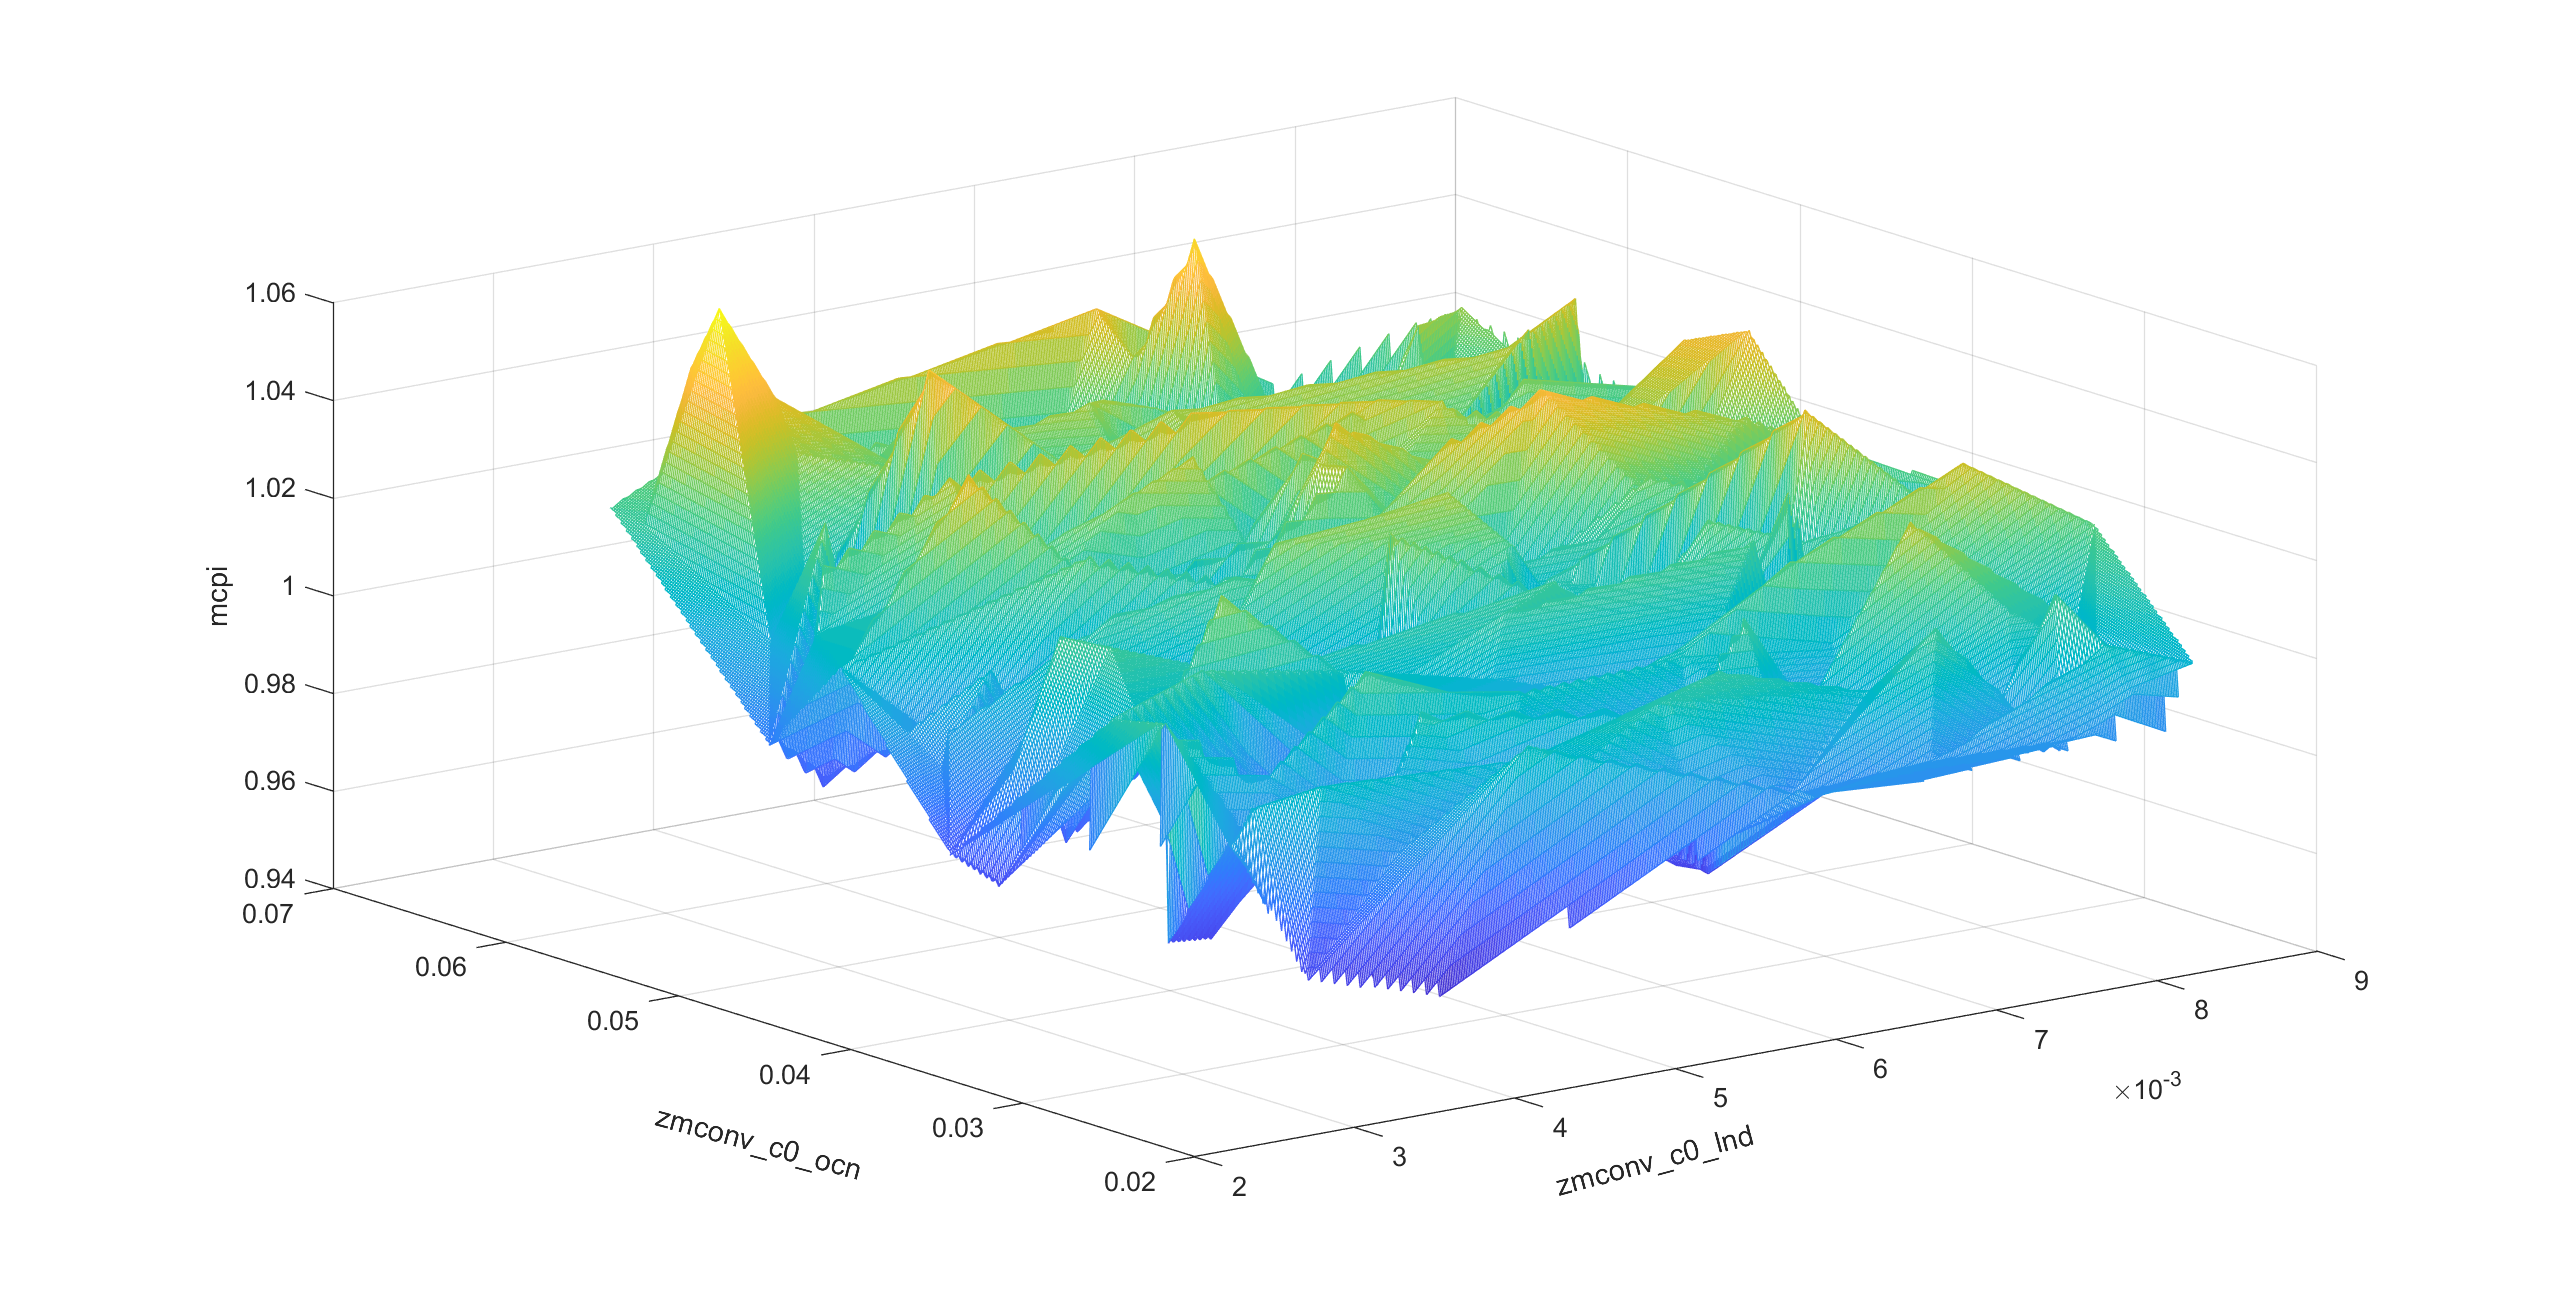
\includegraphics[scale=0.2]{space_SCAM.png}
  \caption{SCAM在二维参数的变化下导致的性能变化}
  \label{fig:soscamspace}
\end{figure}    

\begin{figure}[H]
\centering
\begin{minipage}[t]{0.48\textwidth}
\centering
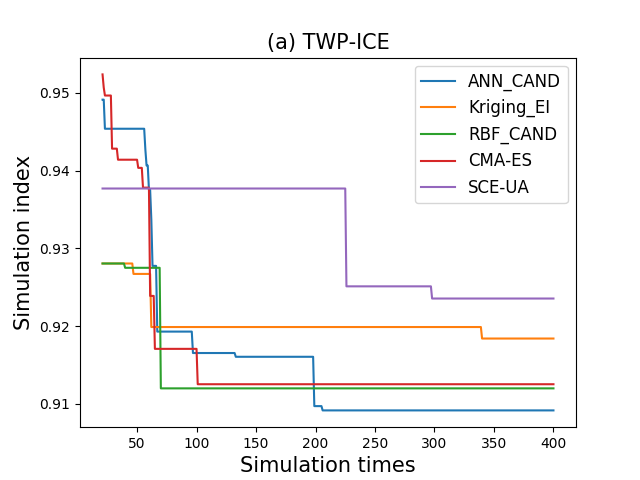
\includegraphics[width=8cm]{figures/twpicescam.png}
%\caption{ZDT2 hypervolume}
\end{minipage}
\begin{minipage}[t]{0.48\textwidth}
\centering
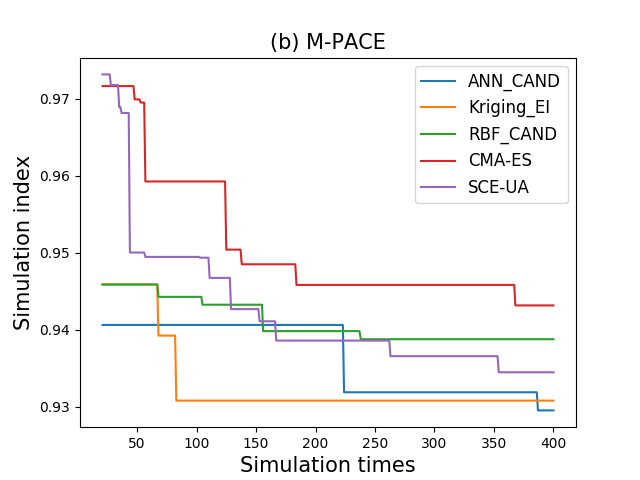
\includegraphics[width=8cm]{figures/mpacescam.png}
%\caption{ZDT2 IGD}
\end{minipage}
\caption{单目标优化算法在TWP-ICE和M-PACE单柱大气模式上的优化结果}
\label{fig:soscam}
\end{figure}

\section{气候系统模式不确定参数的多目标优化方法}
\subsection{多目标优化方法设计}
本文的第一节中叙述了在气候系统模式不确定参数优化中常有多个目标需要同时优化的情况,上文中对单目标代理模式优化和进化算法优化的对比可以看出代理模式优化在复杂问题上大多数情况下都能比进化算法更快地取得相对更好的优化结果,而在Kriging\_EI、RBF\_CAND、ANN\_CAND三个代理模式的评比中本文提出的ANN\_CAND方法在复杂问题中表现较好。在此基础上本小节对上述单目标的ANN\_CAND方法进行扩展,并将扩展后的算法与常见的进化多目标进行对比。另外为了便于下文叙述,在描述多目标优化算法之前,对相关术语进行定义。

定义1 : 非支配解

假设S1,S2为多目标解集中的任意两个点,若对于多目标中的任何一个目标而言,S1的结果都优于S2,则S1支配S2。若S1没有被解集中任何其他的解所支配,则S1为非支配解。

定义2 :  帕累托前沿

帕累托前沿是所有非支配解组成的解集。

多目标优化问题目前最常用的方法是进化多目标算法,例如有NSGAIII (Non-dominated Sorting Genetic Algorithm III)、MOPSO (Multi-objective particle swarm optimization)、MOEA-D (Multi-objective evolutionary algorithm based on decomposition)等算法,其中NSGAIII和MOEA-D算法应用较为广泛。NSGAIII算法是一种带有精英策略的遗传多目标算法,其主要思想是利用hypervolume指标对非支配解进行快速排序,快速获得更全面、更优的非支配解集~\cite{deb2014evolutionary}。MOEA-D算法的主要思想是使用聚合函数将多目标问题转化为多个标量子问题,通过对子问题的优化,不断提高整体优化效果。

面向气候系统模式参数优化,当前多目标算法所存在的问题有:

1.优化迭代步数多。进化多目标算法相比于进化单目标算法,优化收敛性慢,迭代步数多的问题更加显著。从单目标优化问题变成多目标优化问题,所需要的迭代步数是成指数级增长的。

2.基于代理模式的多目标优化算法有待进一步研究。因为传统统计回归方法难以实现高精度的从多个输入向量到多个输出向量之间的回归,所以基于代理模式的多目标优化算法相对欠缺。

%\subsection{多目标优化算法}
本文将ANN\_CAND算法扩展成多目标优化算法(MO-ANN)的伪代码如算法3所示。其主要思想是:(1)应用代理模式优化的思路同时结合进化中多目标优化算法的非支配解排序策略。MO-ANN在每一次寻找当前最优采样点时必须在非支配解中寻找,这样的选择防止选取到的采样点出现一个目标特别好,而另外一个目标极差情况;(2)基于多层感知机神经网络的代理模式能够相对传统的回归方法更好地实现多个输入到多个输出的回归问题。MO-ANN多目标方法的关键步骤解释如下:

1. 非支配解的获取。每一步寻找最优参数将当前所有样本进行比较,找出其中的非支配解。

2. 最优采样点的选择策略。求出非支配解后再对非支配进行排序。非支配解中最好的采样点作为当前已有最优采样点。然后利用文中的扰动方法在已有最优采样点的附近获取更多的候选采样集。

3. 多目标代理模式的应用。多目标代理模式的输入是多维不确定参数,输出为多个目标变量的预测结果。在下一个采样点估计中利用代理模的输出结果和采样点之间的距离为候选集评分。代理模式的多个输出结果的综合如前面在真实采样点中的目标综合方法相同,都默认每个目标的重要程度相当,取多个目标值的平方和再开方。

\floatname{algorithm}{算法}
\renewcommand{\algorithmicrequire}{\textbf{输入:}}
\renewcommand{\algorithmicensure}{\textbf{输出:}}
\begin{algorithm}
        \caption{MO-ANN优化方法}
        \begin{algorithmic}[1] %每行显示行号
            \Require 原模型$F$, 待调参数$X$, MLP神经网络$M$,利用率$weight$
            \Ensure 优化参数
            \State $S \gets InitSamples( F, X )$
            \For{$i = 0 \to T$}
                \State $FitMLP(M, S)$
                \State // 获得当前的非支配解集$X$及其对应的$Y$
                \State Get the current non-dominated solution set $NonDominateX$,$NonDominateY$   
                \State // 利用非支配解集获取下一个最优采样点
                \State $xnew_i \gets \Call {MoCandMethod}{NonDominateX,NonDominateY,MLP,weight}$
                \State $ynew_i \gets F(x_i)$
                \State $S \gets S \cup (xnew_i,ynew_i)$
            \EndFor
            
            \Function{MoCandMethod}{$NDX,NDY,MLP,weight$}
              \State // 将所有的目标综合起来,获取非支配解中最好的$X$
              \For{$i=0 \to nObj$}
                  \State $Y \gets NDY(i)^2 $
              \EndFor
              \State $Y \gets Sqrt(Y)$
              \State $index \gets argmin(Y)$
              \State $current\_bestX \gets X(index)$ 
              \State $CandPointSet \gets [RandPerturbatio(current\_bestX),Xrandom]$
              \State $NobjCandValueSet \gets MLP.predict(CandPointSet)$
              \For{$i=0 \to nObj$}
                  \State $CandValueSet \gets NobjCandValueSet(i)^2 $
              \EndFor 
              \State $dis\_metrics(CandPointSet) \gets distance(CandPointSet,X)$
              \State $metrics \gets weight * CandValueSet + (1-weight) * dis\_metrics(CandPointSet)$
              \State $indict \gets argmin(metrics)$
              \State $CandPoint \gets CandPointSet(indict)$
            \EndFunction
        \end{algorithmic}
\end{algorithm}

多目标的评价标准有很多,例如离散度,世代距离,hpervolume和反世代距离(IGD)等~\cite{riquelme2015performance},其中hypervolume为一个关于非支配解离散度和收敛性的综合指标,因其可以同时考量这两个重要的性能而成为近年来多目标评价指标中最常用的指标之一。IGD指标衡量的是当前获得的假设帕累托前沿与真实的帕累托前沿的距离,是对算法收敛性最好的衡量方法之一,通常hypervolume和IGD配合使用来判断多目标优化方法的优劣。

hypervolume的值为reference point和当前的非支配解围成的超立方体体积,体积越大,说明当前非支配解越接近于真实的帕累托前沿。其公式如下所示:
\begin{equation}
\label{equ:Rasfuc}
H v ( p ) = L e b m \left( \bigcup _ { X \in p } \left[ f _ { 1 } ( X ) , r _ { 1 } \right] \cdot \left[ f _ { 2 } ( X ) , r _ { 2 } \right]  \cdots  \left[ f _ { M } ( X ) , r _ { M } \right] \right)
\end{equation}
其中$M$为多目标的目标个数,$p$为当前获得的近似帕累托前沿,$\left[ f _ { 1 } ( X ) , r _ { 1 } \right] \cdot \left[ f _ { 2 } ( X ) , r _ { 2 } \right]  \cdots  \left[ f _ { M } ( X ) , r _ { M } \right]$为受X支配而不受Reference Point支配的所有点共同围成的超立方体。$Lebm$为勒贝格测度,即在高维空间中的超立方体体积。超立方体体积越大则说明当前获得的近似帕累托前沿与真实的帕累托前沿越相似,优化的效果越明显。

反世代距离评价指标的含义为当前估计的帕累托前沿与真实帕累托前沿的距离,距离越小则说明估计的帕累托前沿越准确。但是在一些复杂的真实应用中,真实的帕累托前沿往往是并不知道的。其公式如下所示。
\begin{equation}
\label{equ:Rasfuc}
\mathrm { IGD ( P , Q ) } = \frac { \sum _ { v \in P } distance ( v , Q ) } { \left| P \right| }
\end{equation}
其中$P$为均匀分布在真实的帕累托前沿上的点,$\left| P \right|$为$P$点集的个数。$Q$为当前算法找到的近似帕累托前沿,$distance ( v , Q )$为$P$中的个体$v$到种群$Q$的欧式距离。

%\begin{figure}[H] % use float package if you want it here
%  \centering
%  \includegraphics[scale=0.6]{all_SCAM.png}
%  \caption{SCAM在二维参数的变化下导致的性能变化}
%  \label{fig:xfig1}
%\end{figure} 
\subsection{多目标优化方法性能评估}
为了评价多目标优化算法的性能和效率,本文将其在ZDT2~\cite{zitzler2000comparison},DTLZ7函数~\cite{deb2002scalable}以及上文提到的SCAM模式上做了以下评测。接下来先简单介绍着两个函数,并叙述了测试结果。

ZDT2优化问题的公式如下所示:
\begin{equation}
\begin{array} { l } { F _ { 1 } = x _ { 1 } } \\ { F _ { 2 } = G ( \vec { x } ) \cdot \left[ 1.0 - \left( x _ { 1 } / G ( \vec { x } ) \right) ^ { 2 } \right] } \\ { G ( \vec { x } ) = 1 + \frac { 9 } { n - 1 } \left( \sum _ { i = 2 } ^ { n } x _ { i } \right) } \\ { 0 \leq x _ { i } \leq 1 , i = 1 , \ldots , n } \end{array}    
\end{equation}

DTLZ7公式如下所示:
\begin{equation}
\begin{aligned} F _ { 1 } ( \vec { x } ) & = x _ { 1 } \\ F _ { 2 } ( \vec { x } ) & = \left( 1 + G ( \vec { x } ) H \left( F _ { 1 } ( \vec { x } ) , G ( \vec { x } ) \right) \right. \\ G ( \vec { x } ) & = 1 + \frac { 9 } { | \vec { x } | } \sum _ { x _ { i } \in \mathbb { T } } x _ { i } \\ H \left( F _ { 1 } ( \vec { x } ) , G ( \vec { x } ) \right) & = M - \frac { F _ { 1 } ( \vec { x } ) } { 1 + G ( \vec { x } ) } \left( 1 + \sin \left( 3 \pi F _ { 1 } ( \vec { x } ) \right) \right) \\ 0 & \leq x _ { i } \leq 1,1 \leq i \leq n \end{aligned}
\end{equation}

多目标问题及其对应的reference point选择如表2.3所示:
\begin{table}[H]
\centering
\caption{多目标优化问题及其reference point选择}  
\begin{tabular}{llll}
\toprule[1.5pt]
样例 & X维度 & 目标维度 & Reference point\\  
\hline  
ZDT2    & 12 & 2 & (11,11)   \\
DTLZ7 & 12 & 3 & (40,40,40)  \\
SCAM & 4 & 4 & (2.5,2.5,2.5,2.5)   \\
\bottomrule[1.5pt]  
\end{tabular}  
\end{table}  

ZDT2,DTLZ7函数的测试结果如图~\ref{fig:mofunctions}。其中NSGAIII和MOEA-D算法的种群数都设置为10,因此图中每一次迭代为10次函数计算。总函数模拟次数也为200次。每10次函数计算之后,进化多目标算法和MO-ANN算法计算一次非支配解的hypervolume和IGD。如前文所述,多目标评价中hypervolume值越大越好,IGD值越小越好,因此本文提出的MO-ANN代理模式多目标优化方法相对于NSGAIII和MOEA-D来说能够更快地提升ZDT2和DTLZ7函数优化效果。
\begin{figure}[H]
\centering
\begin{minipage}[t]{0.48\textwidth}
\centering
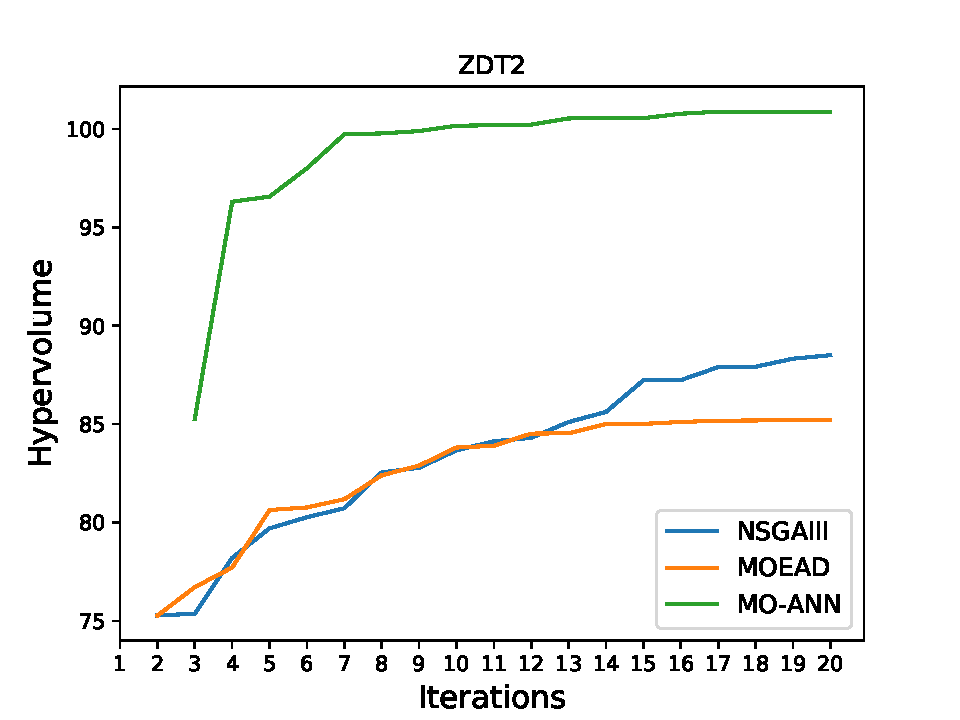
\includegraphics[width=8cm]{figures/hyper_ZDT2.pdf}
%\caption{ZDT2 hypervolume}
\end{minipage}
\begin{minipage}[t]{0.48\textwidth}
\centering
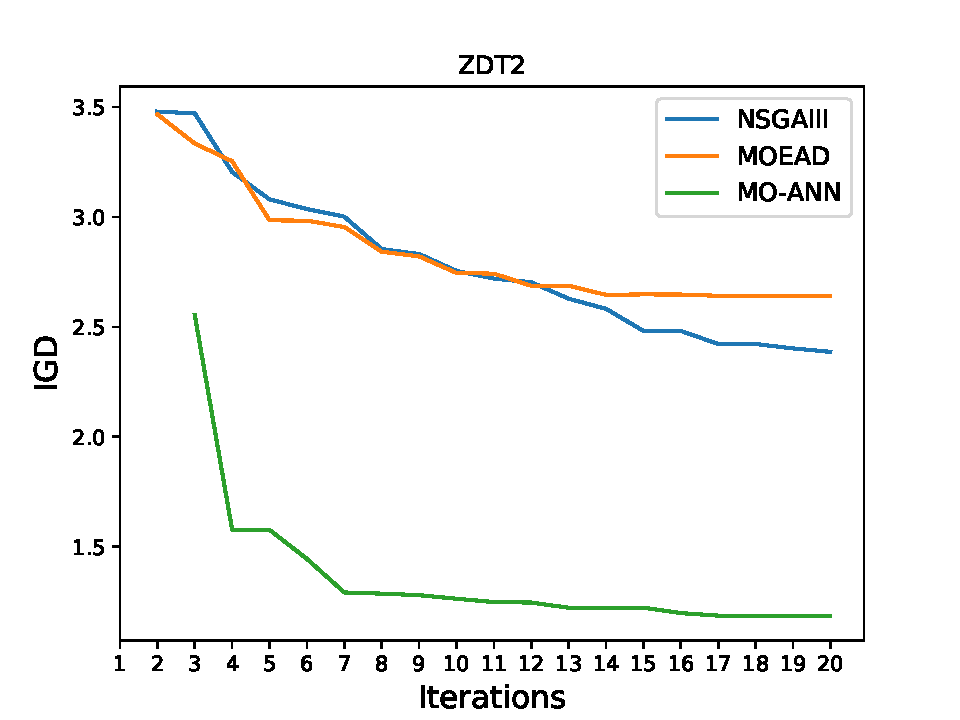
\includegraphics[width=8cm]{figures/igd_ZDT2.pdf}
%\caption{ZDT2 IGD}
\end{minipage}
%\caption{ZDT2函数上多目标优化算法对比}
\\
\centering
\begin{minipage}[t]{0.48\textwidth}
\centering
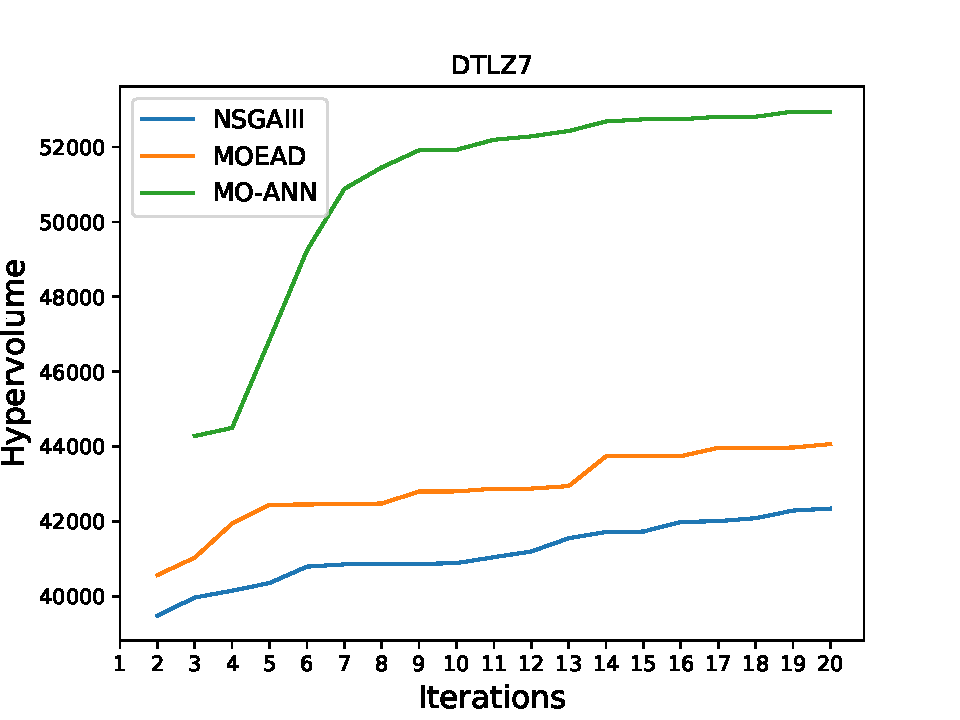
\includegraphics[width=8cm]{figures/hyper_DTLZ7.pdf}
%\caption{DTLZ7 hypervolume}
\end{minipage}
\begin{minipage}[t]{0.48\textwidth}
\centering
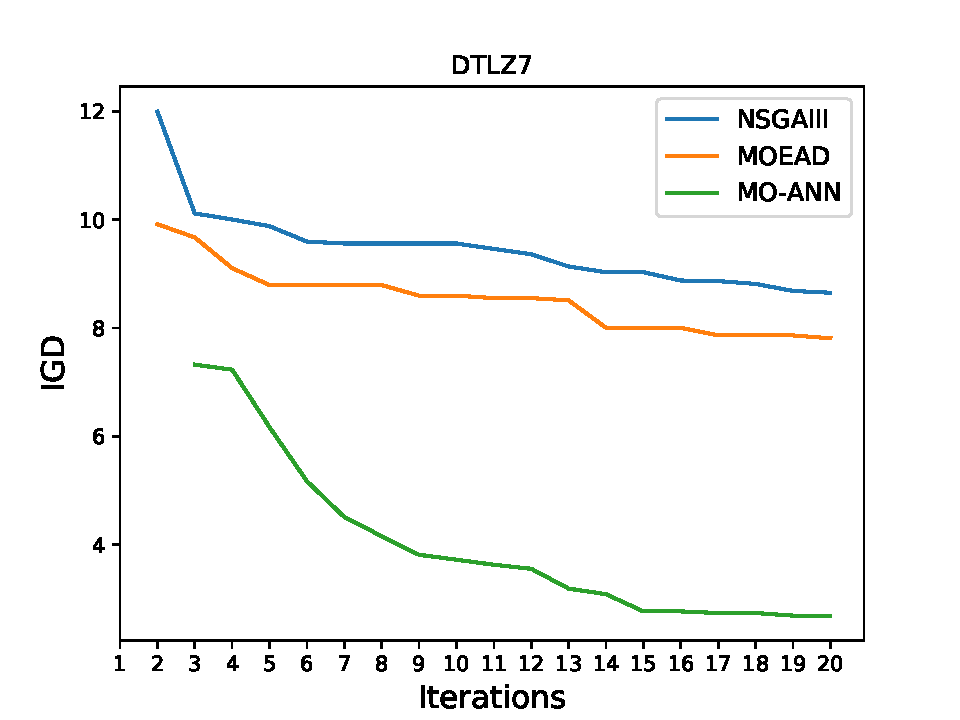
\includegraphics[width=8cm]{figures/igd_DTLZ7.pdf}
%\caption{DTLZ7 IGD}
\end{minipage}
\caption{ZDT2和DTLZ7函数上多目标优化算法对比}
\label{fig:mofunctions}
\end{figure}

为了进一步测试多目标算法在单柱大气模式中的效率,本文接下来将表2.1中的每一个变量的模拟性能作为单独的目标。对表2.2中的不确定参数进行调整,多目标算法评比结果如图~\ref{fig:moscam}。

\begin{figure}[H]
\centering
\begin{minipage}[t]{0.48\textwidth}
\centering
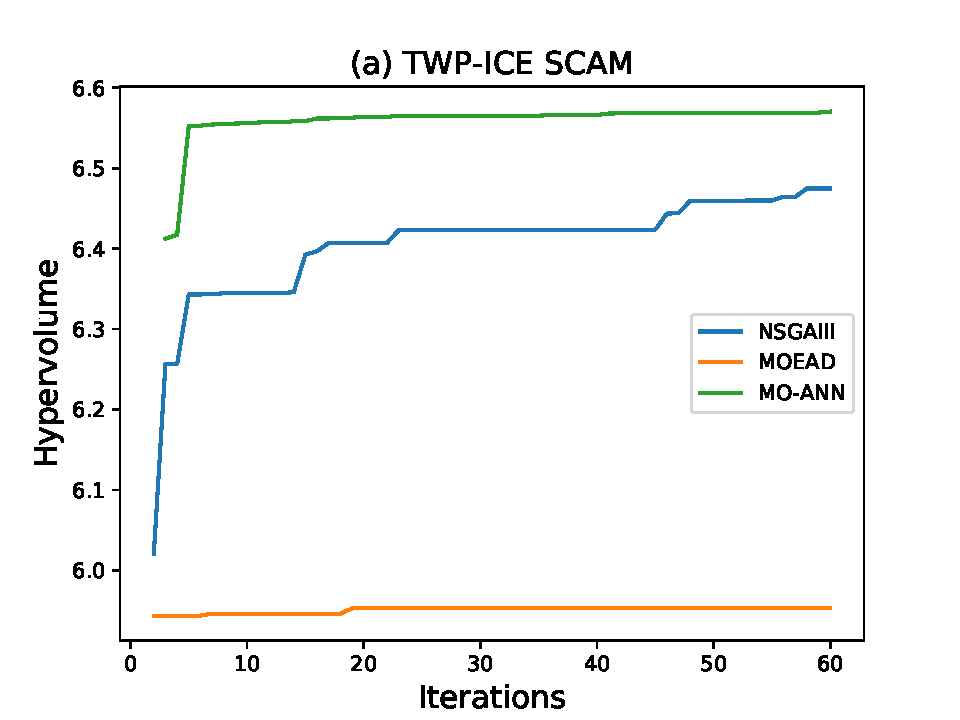
\includegraphics[width=8cm]{figures/MO-TWP.pdf}
%\caption{ZDT2函数上多目标算法的hypervolume}
\end{minipage}
\begin{minipage}[t]{0.48\textwidth}
\centering
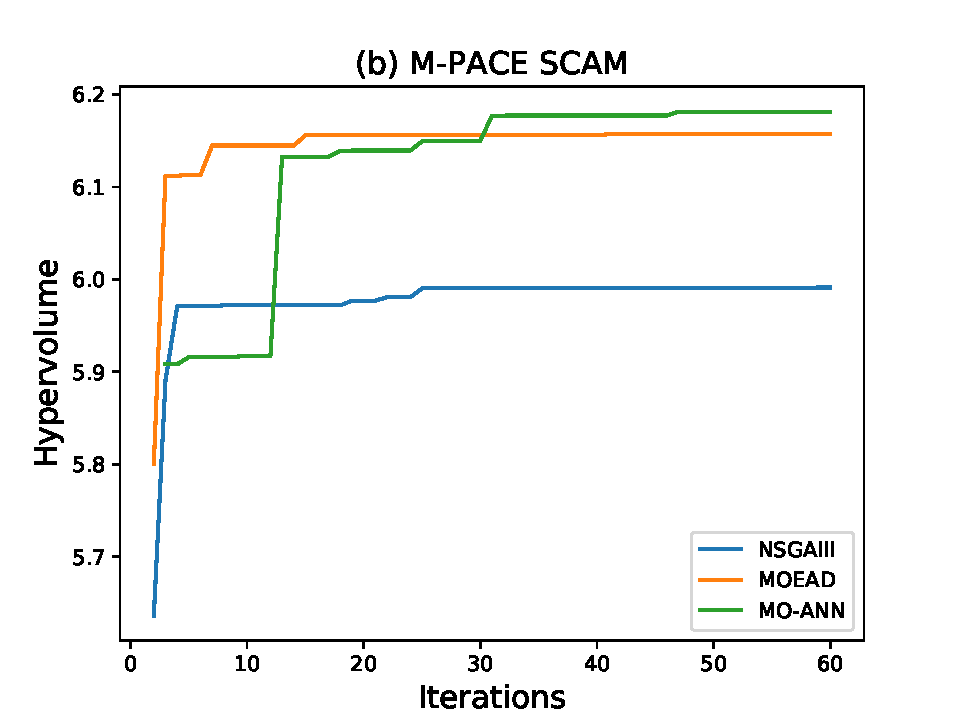
\includegraphics[width=8cm]{figures/ARW-MO.pdf}
%\caption{ZDT2函数上多目标算法的IGD}
\end{minipage}
\caption{TWP-ICE和M-PACE单柱大气模式上多目标优化算法的hypervolume比较}
\label{fig:moscam}
\end{figure}

单柱大气模式无法求出真正的帕累托前沿,因此对于多目标优化算法在SCAM上的评价,本文以hypervolume作为标准。与在ZDT2和DTLZ7上的优化测试相同,这里也将每10次模式运行作为1次迭代,计算一次hypervolume。从图~\ref{fig:moscam}中可以看出在TWP-ICE上MO-ANN能够更快更好地获取更优的非支配解集。在第10次迭代时已经取得较优的结果,而NSGAIII进化多目标算法则优化速度相对缓慢,在第60次迭代时依旧没有完全收敛,MO-ANN收敛速度是它的5倍以上。在M-PACE上的MO-ANN多目标算法的优势虽未能有TWP-ICE上显著,但是也是三个多目标算法中精度最高的算法。

\subsection{基于物理约束的参数优化方法}
如本章第一节中所述,在气候系统模式内有很多物理原理需要遵循,例如大气顶的辐射平衡等,这些物理条件对气候系统模式的模拟性能和模拟稳定性有一定的影响。因此在必要情况下,气候系统模式的参数优化需要考虑物理条件约束的影响。为了使优化算法适应在有约束优化情况下的优化,本节将基于MO-ANN算法进一步设计有约束多目标优化方法。处理有约束优化问题可以分为两大类,第一类是罚函数法,这种方法简单有效,但是针对不同问题,选择合适的罚因子比较困难。第二类方法是将约束问题作为另外一个优化问题,这种方法增加了优化问题的目标,为优化问题带来了一定的难度,但也可以更好的权衡目标和约束之间的关系。

1.罚函数法。罚函数法的思路是如果当前约束得不到满足的话,就将约束乘以一个很大的值加到目标函数上,这样让优化算法记住,此处自变量的选择并不合适。这里根据MO-ANN设计了一个利用罚函数思想的有约束多目标优化算法(MO-ANN-CON-penalty),此算法对于每一个进入代理模式的样本首先计算其约束条件,若约束条件没有满足,则选择一个远大于优化算法因变量的罚因子,将其加到每一个目标变量中。算法的其他部分和MO-ANN保持一致。

2. 约束转化为目标方法。约束转化为目标方法的思路是将约束条件也作为另外一个优化目标。但是在每一次进行非支配排序之前将不满足约束的点从样本中去掉,不让它进入非支配排序。此处的做法也是为了防止迭代在不断进行但是最终没有找到可行解的情况。在对前文MO-ANN算法进行扩展后,转化约束为目标的有约束多目标优化算法(MO-ANN-CON-con2obj)如算法4所示。
重要步骤的解释如下:

(1)可行解进入非支配解排序。每一次在选取当前真实最优采样点时都从当前可行样本中选取非支配解。

(2)目标和约束代理模式的建立。分别为目标和约束构建代理模式,这一点对于气候系统模式的有约束优化问题来说非常重要,因为气候系统模式的约束和输入参数虽关系密切,但并不是一个简单的数学函数表达式,而是一个复杂的经过模式运行和评估所得到的结果,所以为约束也构建代理模式更方便估计输入参数与模式模拟结果之间的关系。


(3)约束转化为目标的最优参数估计。分别用目标代理模式和约束代理模式预测采样候选集中的样本,然后将对应的预测目标和约束组合,然后和前文的MO-ANN一样,选取多目标综合效应好的采样点作为下一个真实采样点。

\floatname{algorithm}{算法}
\renewcommand{\algorithmicrequire}{\textbf{输入:}}
\renewcommand{\algorithmicensure}{\textbf{输出:}}
\begin{algorithm}
        \caption{MO-ANN-CON-con2obj优化方法}
        \begin{algorithmic}[1] %每行显示行号
            \Require 原模型$F$, 待调参数$X$, MLP神经网络$M$,利用率$weight$
            \Ensure 优化参数
            \State $S \gets InitSamples( F, X )$
            \For{$i = 0 \to T$}
            \State //分别为目标和约束建立MLP代理模式
                \State $FitObjMLPModel(M, S)$
                 \State $FitConMLPModel(M, S)$
                 \State Get the non-dominated solution $NonDominateX$,$NonDominateY$ of the feasible solution 
                \State $xnew_i \gets \Call {MoCandConMethod}{NonDominateX,NonDominateY,MLP,weight}$
                \State $ynew_i \gets F(x_i)$
                \State $S \gets S \cup (xnew_i,ynew_i)$
            \EndFor
            \Function{MoCandConMethod}{$NDX,NDY,MLP,weight$}
              \For{$i=0 \to nObj$}
                  \State $Y \gets NDY(i)^2 $
              \EndFor
              \State $Y \gets Sqrt(Y)$
              \State $index \gets argmin(Y)$
              \State $current\_bestX \gets X(index)$ 
              \State $CandPointSet \gets [RandPerturbatio(current\_bestX),Xrandom]$
              \State //利用代理模式估计样本集中的目标和约束
              \State $CandValueSet \gets ObjModel.predict(CandPointSet)$
               \State $CandConSet \gets ConModel.predict(CandPointSet)$
              \State $dis\_metrics(CandPointSet) \gets distance(CandPointSet,X)$
              \State //将约束作为另一个目标,利用代理模式对每个样本集中的样本进行评估
              \State $metrics \gets weight * [CandValueSet$,$Con] + (1-weight) * dis\_metrics(CandPointSet)$
              \State $indict \gets argmin(metrics)$
              \State $CandPoint \gets CandPointSet(indict)$
            \EndFunction
        \end{algorithmic}
\end{algorithm}
\subsection{约束多目标优化方法性能评估}
假设单柱大气模式的模式顶辐射偏差不超过默认实验,辐射偏差的定义为模式顶净短波辐射(FSNT)和净长波辐射(FLNT)之差的绝对值。则上述两种方法在SCAM上的测试结果如下所示。
%\section{自动化的基于ANN代理模式的参数优化平台实现}
\begin{figure}[H]
\centering
\begin{minipage}[t]{0.48\textwidth}
\centering
\includegraphics[width=8cm]{figures/twpconstraint.pdf}
%\caption{ZDT2函数上多目标算法的hypervolume}
\end{minipage}
\begin{minipage}[t]{0.48\textwidth}
\centering
\includegraphics[width=8cm]{figures/constaint3.pdf}
%\caption{ZDT2函数上多目标算法的IGD}
\end{minipage}
\caption{TWP-ICE和M-PACE单柱大气模式上有约束多目标算法的hypervolume比较}
\label{fig:moconscam}
\end{figure}
从图~\ref{fig:moconscam}可以看出在MO-ANN算法上扩展而成的有约束优化算法MO-ANN-CON-penalty和MO-ANN-CON-con2obj在M-PACE上的性能表现较为相似,但是在更复杂的TWP-ICE上,MO-ANN-CON-con2obj方法表现更好。

\section{气候系统模式不确定参数优化方法整合}
前文叙述了在气候系统模式的单目标、多目标以及有约束参数优化情景下,各类基于多层感知机神经网络的代理模式优化方法是如何设计的以及它们与传统代理模式优化以及常用进化算法在复杂数学函数和单柱大气模式上的评估。本节将介绍各类优化算法整合与总体设计。
\begin{figure}[H] % use float package if you want it here
  \centering
  \includegraphics[scale=0.7]{figures/surrogateprocess.pdf}
  \caption{面向气候系统模式的代理模式参数优化方法类图}
  \label{fig:optclass}
\end{figure}   
整合以上单目标、多目标以及有约束优化方法将优化算法通用化,使其能够根据优化场景自动选择合适的优化算法。整合后的优化方法类图如图~\ref{fig:optclass},主要分为以下几个部分。

1.优化总流程的调度(Optimization)。此部分将气候系统模式参数优化的每一个流程串联在一起,包括从一开始的拉丁超立方采样到当前最优采样点的评估,再到下一个真实采样点位置的选取等循环过程,从所选的优化问题可以得出当前是需要单目标优化,多目标优化还是有约束优化,分别选择不同的优化算法对优化问题不断进行探索。

2.优化问题定义部分(Problem)。此部分定义问题的输入维度,输出维度,参数的取值范围,所需要优化问题的评估等,在数学函数上此评估仅为一次函数值的计算,但是对于气候系统模式参数优化来说,这意味着一次模式的运行,模式输出结果的后处理与优化评价标准的获取。在气候系统模式中的一次评估(evaluation)具体步骤有:将当前参数取值匹配到模式中的参数输入文件如namelist中,然后自动启动模式的运行(run\_model),根据优化评价标准设计模式的评估函数(get\_metrics)并获取优化指标的值。

3.通用的代理模式部分(Generalizer)。初始采样所获取的采样点赋值给sample\_x和samples\_y,后续每添加一个采样点都利用incorporate\_new\_sample将其加到已有样本库中。每一个最新样本点的位置都是由它调用优化策略模块(CAND)获取的。它的surrogate部分由NNRegression具体实现。代理模式的fit过程将当前所有样本用来拟合成为一个回归器,代理模式的predict环节利用当前所建立的回归器对未知点进行预测。多层感知机神经网络由输入层,隐含层和输出层共同构成,其中除了输入层之外每一层都带有非线性激活函数,使得模型更能够适应非线性较强的特性表达。特别值得注意的是这里的代理模式的拟合过程,并不是一般机器学习意义上寻求偏差和方差的平衡情况,这里仅仅将其作为一个回归器来使用。所以每一步的拟合过程要尽量准确,和传统代理模式的响应面意义相似。面向气候系统模式物理参数优化的多层感知机代理模式输入为相应的物理参数,输出为多个气候变量的模拟能力,用代理模式来估计物理参数对气候模式模拟性能的影响。

4.优化算法的优化策略部分(CAND)。此部分主要是各个代理模式优化算法的最优样本选择策略。在单目标、多目标、有约束优化的实现过程中有些细节上的调整。估计下一个最优采样点的步骤有:根据当前所有的samples\_x,samples\_y,
samples\_constratint等选取当前真实最优的样本,对此最优样本进行扰动获得待评估参数组合(candidate\_samples\_x),用当前拟合好的代理模式(surrogate)以及离已有样本库的距离对其进行评估。评估结果好的将有机会被带入真正的气候系统模式中进行真实的采样。
   
\section{本章小结}
本章首先分析了气候系统模式中面临的单目标优化、多目标优化以及有约束优化问题,总结了当前各类优化问题分别有哪些常用的算法,对广泛应用的算法进行了简要描述。然后本章对当前优化方法在复杂气候系统模式上使用所存在的问题做了简要分析,并提出了基于多层感知机神经网络(MLP)的代理模式优化算法。此算法利用基于MLP的回归模型代替真实气候系统模式预测最优采样点,每增加一次采样点更新一次代理模型。最后本章将基于MLP代理模式的优化算法与常用优化算法在复杂函数和单柱大气模式上的优化性能进行了对比,并详细叙述了面向气候系统模式参数优化方法的整合与实现。

单目标的ANN\_CAND算法相对CMA-ES和SCE-UA算法来说,它能够实现更快的收敛速度,相对于Kriging\_EI、RBF\_CAND来说,它在精度上有所提升。根据单目标优化算法的评比结果将ANN\_CAND扩展为多目标代理模式优化算法MO-ANN,此方法与当前常用的NSGAIII和MOEA-D算法对比结果表明此方法表现良好,在单柱大气模式上收敛速度最好可相对NSGAIII提升5倍以上。最后为了处理气候系统模式中的物理约束问题,本文将MO-ANN扩展成为基于罚函数和转化约束为目标的约束优化方法,两个方法在单柱大气模式上的比较结果表明转化约束为目标的方法在复杂优化场景精度更高。

综上所述基于多层感知机代理模式的优化算法能够更加全面有效地应对复杂场景的参数优化问题。


%本章的详细结论如下所示:
%(1)单目标优化中CMA-ES算法
\chapter{气候预测集合初值扰动方法设计}
\label{cha:china}
\section{当前初值集合方案存在的问题}

混沌系统的初值不确定性会导致系统模拟结果有巨大的差异。而气候系统模式中的初值误差也会因为在系统内的非线性叠加而导致模拟结果与真实气候状态相距甚远。当前的气候预测系统中的初值大多是经过同化后的相对准确的结果。即便如此,改进后的初值相对于真实的大气状态还是有一定的差别。此时为了更好地改进预测结果,初值集合方案被提出。它是通过对初值进行微小的扰动,用扰动后的多个初值,进行集合预报,用集合预报的结果来代替单一的预报结果。特别是针对受到初始条件不确定性影响很强的耦合模式而言,初值集合预报更加必要。集合预报的方式已经应用在各大气象预报中心,是提高气象预测系统预测性能的一个重要方法。但是由于前面提到的气候系统模式的高计算代价以及气候预测的模拟时间较长等原因,面向气候预测的初值集合方案研究还有所欠缺。

第一章中简单介绍了天气初值集合方法和现有的气候集合方法。其中 滞后平均法方法理论基础不是特别完备,奇异向量法(SVs)实现上相对困难且计算代价高。因此本文试图将增长模繁殖法(BGM)应用于国家气候中心的季节集合预报。本文将探讨与BCC-CSM当前正在使用的LAF集合方法相比,BGM方法是否可以提高短期气候预测技巧。本章接下来的结构安排如下。第2节介绍了BCC-CSM气候系统模式和面向气候预测的BGM集合方法。第3节介绍了试验设计和集合评价标准,第4节将BGM和LAF集合方法预测结果进行了评估。
%第4节介绍了结果。

\section{基于气候系统模式改进的增长模繁殖法}
\subsection{BCC-CSM气候系统模式介绍}
本文中所使用的气候系统模式是由我国国家气候中心开发的BCC-CSM2-MR~\cite{wu2019beijing},它参加了国际耦合模式比较计划第六阶段(CMIP6),是在参加过CMIP5的BCC-CSM1.1m~\cite{wu2013global,xiao2013introduction}和早期的季节气候预测系统~\cite{liu2014relationships,liu2015performance}的基础上改进的模式。BCC-CSM2-MR和BCC-CSM1.1m之间的主要差异是大气和陆面模块中的物理过程。在大气模型中,垂直层的层数从26层增加到了现在的46层,并且将从对流源产生的重力波阻力引入了平流层。此外,BCC-CSM2-MR还更新了大气中深对流和云的参数化方案,并且增添了气溶胶的间接影响。BCC-CSM2-MR的陆地部分是BCC-AVIM2.0,它是在早期版本BCC-AVIM1.0上的改进,包括积雪、植被和土壤冻融过程。BCC-CSM2-MR的海洋和海冰模型组件与BCC-CSM1.1m相同。海洋模型是模块化海洋模型版本4(MOM4),其垂直层数为40,由地球物理流体动力学实验室(GFDL)开发。海冰组件是由GFDL开发的海冰模拟器(SIS)。海洋和海冰模型的水平分辨率为1$^\circ$经度,1/3$^\circ$纬度。与BCC-CSM1.1m相比,新的BCC-CSM2-MR在模拟平流层准两年振荡(QBO),东亚降水和地面气温的长期趋势方面取得了显著的进步~\cite{wu2019beijing}。BCC-CSM2-MR目前正在调研进一步提升季节气候预报技巧的方法,为新一代BCC-CSM气候预报系统做准备。
\subsection{面向气候预测的增长模繁殖法初值扰动集合设计}

增长模繁殖法首先在天气初值集合扰动方法中被提出。它的主要思路是利用对初始场的随机扰动来模拟初始场的误差,并通过反复将扰动在模式中进行繁殖而获取快速增长的误差,以此作为集合预报的初始场的最终扰动~\cite{toth1997ensemble}。其一般流程如下所示:

(1) 初始场上叠加(扣除)随机扰动

(2) 将扰动场和控制场一起往前积分一段时间

(3) 获取扰动场和控制场的差,作为此繁殖循环的增长模

(4) 调整增长模尺度使其与初始扰动在均方根意义上相当,将调整后的增长模作为下一次繁殖循环的扰动

(5) 重复2-4步骤,直到增长模的增长率饱和,此时获得的最终扰动,即为集合预报初始场的最终扰动。

增长模繁殖法的示意图如~\ref{fig:bgm}所示:
\begin{figure}[H] % use float package if you want it here
  \centering
  \includegraphics[scale=0.8]{figures/bgm.jpg}
  \caption{BGM流程示意图}
  \label{fig:bgm}
\end{figure}

研究表明,在增长模繁殖法中的关键技术主要有以下三点~\cite{郑峰2008集合预报初值扰动在天气预报中的应用研究进展}:
(1) 繁殖循环的每一个循环的长度是多少,总繁殖周期是多长;
(2) 初始扰动该如何选择;
(3) 如何选择增长模的动态调整方法。

在天气集合预报中每一个繁殖循环的长度通常为6h或者12小时,增长模增长率大约在3-4天之后就会饱和~\cite{toth1997ensemble,zhang2010beating}。而如此之快的饱和速度对于气候预报明显是不适合的,因为在气候预报中不仅有快速变化的物理过程,还有相对慢变化的过程,增长模的增长率过早地达到饱和,会使得慢变化过程中的特征和误差没有被完全捕捉。另外有研究表明不同的动力框架应选取不同的繁殖循环长度,且在耦合模式中需要更长的繁殖循环长度~\cite{yang2006enso,baehr2013ensemble}。根据以上的介绍,针对于BCC-CSM气候系统模式,本文通过实验调整,找到了最优的繁殖循环时间为每5天为一个循环,共繁殖4次,总繁殖周期为20天。增长率的计算公式将在下面和动态调整方法一起介绍。
增长率随繁殖循环变化图如~\ref{fig:bred cycle}。
\begin{figure}[H] % use float package if you want it here
  \centering
  \includegraphics[scale=0.5,trim=0 0 0 30,clip]{breeding_cycle.png}
  \caption{增长率随繁殖循环变化图}
  \label{fig:bred cycle}
\end{figure}

初始扰动的获取,在天气中一般的选择是扰动某单个或者多个变量,使其尺度与模式初始场预报1小时所产生的误差在同一等级。而在气候中这一做法显然不合理。其主要原因是由于气候预报主要关注的是较长时间尺度的气候特征,在1小时预报尺度上的误差很大,与真实的初始场可能存在的误差差距很大。本文这里的做法是对初始场随机扰动使其与全球观测误差分布尺度相当。另外为了使得集合预报在多个变量上都取得较好的结果,本文选择的扰动变量有纬向风,径向风,温度,相对湿度。模式初始场是一个瞬时文件,本文选择的气候变量都是三维的(经度,纬度,垂直高度)变量,扰动也是三维的随机扰动。这样能够对不同垂直层的气候都有一个微小的扰动,让扰动场更有可能包含真实的气候初始场。

增长模动态调整方法通常是将增长调整到与初始扰动均方根在同一个量级,此处面向气候的BGM方法与天气中保持一致。这个操作的意义在于使得快速增长的误差被保留而慢增长的误差在循环中逐渐被忽略。另外扰动变量的均方根的计算为所有垂直层的平均均方根。

前文介绍了面向气候预测的BGM方法的关键技术,接下来将叙述方法的实现细节。方法的实现共分为以下三个主要部分:初始扰动生成,繁殖循环流程建立和并行集合预测提交。其中初始扰动的获取利用NCL(NCAR Command Language)和NCO(netCDF Operators)来实现的,繁殖循环流程建立和并行集合预测提交则都是利用Shell脚本来控制的。

初始扰动部分生成了4对扰动,让每个初始扰动并行进入繁殖循环流程,它包括气候系统模式的自动匹配提交,增长模的获取以及动态调整因子和增长率的计算等模块。由上文可知,在获取初始扰动场之后要将扰动场和控制预报一起往前报一个繁殖循环长度。这里通过Shell脚本自动更改气候系统模式提交的日期,运行的时长以及所需要的初始场等信息。在判断扰动预报和控制预报一个繁殖循环都运行完之后将扰动预报和控制预报相减获取增长模。按照下述公式计算增长率和动态调整因子。假设初始扰动为$p_0$,它在均方根意义上的大小可由以下公式表达。
\begin{align}
&  { E } \left( p _ { 0 } \right) = ({\frac{ \sum _ { i = 1 } ^ { N } p _ { 0 i } ^ { 2 }}{N}})^ { 1 / 2 } 
\end{align}
其中$N$为全球格点数,$p_{0i}$为i格点上的扰动大小。设第$t$步繁殖循环之后所获得的扰动场如下所示:
\begin{align}
& p _ { t } ^ { \prime } = f _ { t } ^ { \mathrm { perb } } - f _ { t } ^ { \mathrm { cntl } } 
\end{align}
其中$f _ { t } ^ { \mathrm { perb } }$为$t$时刻的扰动预报场,$f _ { t } ^ { \mathrm { cntl } }$为$t$时刻控制预报场。则$t$时刻的动态调整系数如下所示:
\begin{align}
& { rescaleFac } = \frac { E \left( p _ { 0 } \right) } { E \left( p _ { 1 } \right) } 
\end{align}
增长率的计算公式如下:
\begin{align}
& growthRate _ { t } = \frac { E \left( p _ { t } ^ { \prime } \right) } { E \left( p _ { t } \right) } = \frac { E \left( p _ { 0 } \right) } { resaleFac _ { t } E \left( p _ { t } \right) } 
\end{align}
其中$E \left( p _ { t } \right) = E \left( rescaleFac _ { t - 1 } p _ { t - 1 } ^ { \prime } \right)$,为$t-1$步输出模经过调整得到的第$t$步循环的输入模。

当所有的繁殖循环完成,扰动场都已准备完毕,将其加到起始预报当日的初始场上,面向气候的增长模繁殖法共获得了8个扰动场,此时利用Shell脚本控制所有正扰动预报和负扰动预报以及控制预报的提交,得到9个集合预报的结果。整合以上流程,面向气候预测的BGM初值集合预报流程示意图如图~\ref{fig:bgm ensem fore}所示。

\begin{figure}[H] % use float package if you want it here
  \centering
  \includegraphics[scale =0.37]{figures/初值集合预报示意图.pdf}
  \caption{BGM初值集合预报示意图(d为天数,m为月份)}
  \label{fig:bgm ensem fore}
\end{figure}

\section{试验设计与集合评价标准}
为了证明本文所提出的面向气候的BGM方法的有效性,下面将此BGM方法与国家气候中心正在使用的面向气候的LAF进行对比。此LAF方法集合成员的初值选取分别相对滞后3天。比如说第一个成员相对于控制预报滞后3天,第二个成员则滞后6天,依次类推。此方法所依赖的原理是相近的天数的初值相似程度高,并且有一定的离散度。接下来将详细介绍两种集合方法的试验设计和评价指标。

1. 试验设计。回报试验的时间选在2000年-2014年,分别从每年的5月1日报到8月31日。两种集合方法的成员数目相同,都是8个扰动预报加一个控制预报。本文所评价的气候变量及其观测数据的来源见表~\ref{tab:eva varibles}。

\begin{table}[htb]
\centering
\caption{气候变量及其对应的观测数据}  
\begin{tabular}{lll}
\toprule[1.5pt]
变量名称 & 变量含义 & 观测\\  
\hline  
T850     & 850hPa Temperature   & ERAI-Interim\\
    U850   & 850hPa zonal wind  & ERAI-Interim\\
    U200    & 200hPa zonal wind    & ERAI-Interim\\
    V850     & 850hPa meridional wind   & ERAI-Interim\\
    Z500     & 500hPa geopotential height  & ERAI-Interim \\
    PRECT & precipitation & GPCP \\
    TREFHT & surface air temperature(SAT) & ERAI-Interim\\
\bottomrule[1.5pt] 
\label{tab:eva varibles}
\end{tabular}  
\end{table}

2.集合评价指标。集合结果的评价一般应有两个方面,一是确定性预报的结果,即将集合成员的结果综合成一个确定的预报结果。二是概率性预报结果,即提供某一事件出现的可能性等。本章以确定性评价指标为主,概率性指标为辅对两种集合方法进行评比。

(1)确定性评价指标。这里的确定性预报结果仍使用的集合平均。衡量确定性预报结果的指标有RMSE(Root mean square error)、TCC(Temporal correlation coefficient)、离散度等。RMSE和TCC都是将集合平均结果与观测做对比以检验哪一组结果离观测更加接近。集合离散度计算的是集合本身的标准偏差,标准偏差越大则说明集合成员之间的差异大,集合平均的结果可信度越小,反之则反。通常预报员在进行确定性预报时要同时结合集合离散度和集合平均等结果共同作出决策。RMSE计算如公式~\ref{equ:RMSE}所示。
\begin{equation}
\label{equ:RMSE}
R M S E = \sqrt { \frac { \sum _ { i = 1 } ^ { N } \left(  w(i)  (  x _ { i } - f _ { i } ) \right) ^ { 2 } } { N } }
\end{equation}
其中$N$为预报格点总数,$x _ { i }$为$i$格点上的观测值,$f _ {  i }$是$i$格点上的模式预测值。$w(i)$为格点权重。RMSE用来衡量观测与预报之间的距离,距离越小,预报能力越强。
每个网格的TCC的计算如公式~\ref{equ:TCC i}。
\begin{equation}
\label{equ:TCC i}
T C C _ { i } =  \frac { \sum _ { j = 1 } ^ { M } \left( _ { X _ { i , j } } - \overline { x _ { i } } \right) \left( f _ { i , j } - \overline { f _ { i } } \right) } { \sqrt { \sum _ { j = 1 } ^ { M } \left( x _ { i , j } - \overline { x _ { i } } \right) ^ { 2 } } \times \sqrt { \sum _ { j = 1 } ^ { M } \left( f _ { i , j } - \overline { f _ { i } } \right) ^ { 2 } } }
\end{equation}
其中$x _ { i , j }$为$i$格点$j$时间上的观测,$x _ { i }$为$i$格点上的观测平均值。$ f _ { i , j }$为$i$格点$j$时间上的模式预测值,$f _ { i }$为$i$格点上的预测平均值。
若要计算区域或者全球平均时也需要考虑每个格点的权重。公式如下所示:
\begin{equation}
\label{equ:Rasfuc}
T C C = \frac { \sum _ { i = 1 } ^ { N } w(i) T C C _ { i } } { \sum _ { i = 1 } ^ { N } w(i) }
\end{equation}
其中$N$为格点总数,$w(i)$为格点权重。TCC指标能够在统计意义上较好地衡量每个格点的异常情况,得到完整的空间评分技巧分布。

(2)概率性评价指标。Brier评分是集合概率性评价的常用指标,其计算方法如公式~\ref{equ:Brier}所示:
\begin{equation}
\label{equ:Brier}
B S = \frac { 1 } { n } \sum _ { i = 1 } ^ { n } \left( f _ { i } - o _ { i } \right) ^ { 2 }
\end{equation}
其中,$n$为预报次数,$f _ { i }$是第$i$次预报的事件发生概率,$o _ { i }$为第$i$次观测的概率,如果事件发生,$o _ { i }$等于1,若没有发生,则为0。BS的结果在0-1之间,其值越小表明预测概率与观测越接近,预报技巧越高。

\section{增长模繁殖法集合预测效果评估}
为了更好地对BGM和LAF的结果进行分析比较,这里分别对两个集合确定性预报和概率性预报结果进行检测,确定性预报检测的流程如下所示。首先本文将计算RMSE和TCC指标,并画出全球空间分布图,从全球平均RMSE和TCC等指标本文能够初步判断两个集合的全球平均预报能力,空间分布图又提供了全球每个格点的情况,根据空间分布图本文能够对不同区域两种集合方法的预报能力有了进一步的认识。此时再利用TCC显著性检验挑出通过检验的区域,分析区域内集合预报技巧。此分析流程从总体到局部,详细的对集合结果做了多方位的评价,分析的输出为可视化的图形,直观且容易理解。

图~\ref{fig:global rmse}中分别展示了BGM和LAF集合预报的全球降水,地表温度、850hPa径向纬向风、500hPa位势高度、200hPa纬向风的全球平均分布的RMSE差,如果差小于0的话,则说明BGM集合方案的RMSE要小于LAF集合方案的RMSE,即BGM方法优于LAF方法。从图~\ref{fig:global rmse}(a)中可以看出两个集合方法对降雨的确定性预报差距不是很明显,除了在赤道太平洋区域略有变化。图~\ref{fig:global rmse}(b)中显示BGM预测的地表温度在亚洲东北部相对LAF有较为明显的提升。850hPa径向风在全球的中高纬度地区相比LAF有所提高,而850hPa纬向风和500hPa位势高度在北半球的大部分区域都有显著的改善。200Pha纬向风在北半球中纬度地区改善明显。从图中可以看出BGM方法相比LAF在预报后的第一个月中可以有效地减小对流层低层和高层纬向风以及对流层中层的位势高度的模型误差。

为了探索两个集合方法在起报随时间往后的月份(lead month)中表现情况,图~\ref{fig:global rmse lead time}中展示了两个集合方法的所有预报月份的200hPa纬向风、500hPa位势高度、850hPa经纬向风的全球平均RMSE。从图中可以看出BGM在这四个变量的预报的第一个月中都有明显的提升,且500hPa位势高度在所有预报月份中都相对LAF预测结果变好。

\begin{figure}[H] % use float package if you want it here
  \centering
  \includegraphics[scale=0.8,trim=1 50 1 75,clip]{Fig2_dif_rmse_May_diff_six.eps}
  \caption{BGM和LAF在5月的PRECT、SAT、U850、V850、Z500、U200的全球RMSE差异分布}
  \label{fig:global rmse}
\end{figure}

\begin{figure}[H] % use float package if you want it here
  \centering
  \includegraphics[scale=0.45,trim=1 110 1 150,clip]{figures/Fig3_dif_rmse_May_Aug_series.eps}
  \caption{BGM和LAF在5月到8月的U200、Z500、U850、V850全球平均RMSE差异}
  \label{fig:global rmse lead time}
\end{figure}

RMSE衡量的是观测值与预测值的相对差值,TCC则充分考虑两个集合预测结果在空间上的相似程度。从图~\ref{fig:TCC four vari}中可以看出在5月份所有变量在北半球大陆通过TCC显著性检验的区域都是BGM集合比LAF更多。对于850hPa径向风来说,BGM集合预报在中国北部,热带西太平洋比LAF集合预测的TCC更显著。对于850hPa纬向风BGM方法在欧洲和西太平洋相对LAF方法有所提升。而500hPa位势高度和200hPa纬向风在全球大部分区域BGM比LAF的TCC都要更好,尤其是在欧亚大陆。

\begin{figure}[H] % use float package if you want it here
  \centering
  \includegraphics[scale=0.7,trim=1 40 1 50,clip]{figures/Fig4_dif_cor_May_circulation.eps}
  \caption{5月V850、U850、Z500、U200的TCC空间分布(阴影区域置信水平高于90\%)}
  \label{fig:TCC four vari}
\end{figure}

\begin{figure}[H] % use float package if you want it here
  \centering
  \includegraphics[scale=0.45,trim=1 10 1 16,clip]{figures/Fig5_dif_cor_May_Aug_series.eps}
  \caption{BGM和LAF在欧亚大陆和西太平洋区区域平均TCC差异}
  \label{fig:Tcc eura and wes pac}
\end{figure}

考虑到欧亚大陆中高层大气环流和西太平洋低层风对亚洲气候的影响,本文进一步关注U200和Z500在欧亚大陆(50$^\circ$-120$^\circ$E 35$^\circ$-60$^\circ$N)以及U850和V850在西太平洋(125$^\circ$-150$^\circ$E, 0-25$^\circ$N) 区域的平均TCC结果。

如图~\ref{fig:Tcc eura and wes pac}(a)所示,500hPa位势高度和200hPa纬向风在所有月份都变好明显。而在西太平洋区域850hPa经纬向风只在5月份BGM方法有所提升(图~\ref{fig:Tcc eura and wes pac}(b))。因此,BGM相对LAF集合方法对欧亚大陆对流层中上层环流的集合预测效果更好,影响时间更长。

\begin{figure}[H] % use float package if you want it here
  \centering
  \includegraphics[scale=0.8,trim=1 125 1 130,clip]{figures/Fig6_dif_cor_May_EA.eps}
  \caption{东亚地区降水和地表温度TCC}
  \label{fig:Tcc of ea pr and sat}
\end{figure}
欧亚大陆BGM方法预报技巧的提升说明了BGM可能对于地表气候的模拟有良好的效果。图~\ref{fig:Tcc of ea pr and sat}显示了BGM和LAF方法在亚洲降水和温度上的TCC空间分布图,从图中可以看出BGM相比LAF在亚洲东北部,中国北方和西太平洋区域预报能力更好。因此可以看出本文所设计的BGM方法是一种有效提升亚洲区域预报能力的方法。

本文选取亚洲西北区域(60$^\circ$-100$^\circ$E, 50$^\circ$-70$^\circ$N),亚洲东北(100$^\circ$-140$^\circ$E, 50$^\circ$-70$^\circ$N),中国北方(100$^\circ$-120$^\circ$E, 30$^\circ$-42$^\circ$N)以及西太平洋区域计算区域平均的降水(PR)和地表温度(SAT)从2000到2014年每年5月的时间序列。由图~\ref{fig:pre and sat corre}可知,BGM预测的亚洲西北部、华北和西太平洋5月降水年际变化较LAF预测的更符合观测结果(图~\ref{fig:pre and sat corre} a,c), 三个区域降水的时间相关系数分别为0.51、0.52和0.62,远高于LAF预报与观测的时间相关系数。BGM集合还在东亚北部、华北、西太平洋地区重现了更为合理的地表温度年际变化,相关系数别为0.62、0.82、0.47(图~\ref{fig:pre and sat corre} d,f)。它们都高于LAF集合预测与观测值之间的时间相关性。BGM集合预测的这些区域降水和地表温度能力的提高与欧亚大陆的Z500和U200以及西太平洋的U850和V850等大气环流的改善是一致的。

\begin{figure}[H] % use float package if you want it here
  \centering
  \includegraphics[scale=0.8,trim=1 50 1 30,clip]{figures/Fig8_May_BGM_LAF_2000_2014.eps}
  \caption{降水和地表温度异常相关系数}
  \label{fig:pre and sat corre}
\end{figure}

夏季亚洲气候的预测对于以一个月为主导时间的BCC-CSM季节预测系统来说仍然是一个挑战~\cite{liu2015performance}。如图~\ref{fig:summer pre and sat} a和b所示,LAF和BGM集合预测的东亚降水预测能力都较低。BGM和LAF集合方法在印度、阿拉伯海和中国南海的地表温度预报能力中都表现出了很高的水平,但在东亚大陆的预报水平却很低(图~\ref{fig:summer pre and sat} d,e)。

另外图~\ref{fig:BS}也分别展示了U200、Z500、U850和V850的概率性集合预报评测Brier评分的结果。结合图~\ref{fig:TCC four vari}和~\ref{fig:global rmse lead time}可以看出概率性预报评价方式Brier评分的结果与确定性集合方法中模拟结果优劣的趋势非常相似,U200、Z500、U850、V850四个变量都是第一个月BGM相对LAF变好趋势明显,Z500和V850变好的时间可以持续更长。因此在后续的集合评价中本文延续了确定性集合评价方法。

\begin{figure}[H] % use float package if you want it here
  \centering
  \includegraphics[scale=0.8,trim=1 120 1 130,clip]{figures/Fig7_dif_cor_JJA_EA.eps}
  \caption{夏季东亚地区降水和地表温度TCC}
  \label{fig:summer pre and sat}
\end{figure}
%其中U200,Z500,U850,V850的阈值选择为
\begin{figure}[H]
\centering
\begin{minipage}[t]{0.48\textwidth}
\centering
\includegraphics[width=8cm]{figures/brier-15-U200.pdf}
%\caption{DTLZ7 hypervolume}
\end{minipage}
\begin{minipage}[t]{0.48\textwidth}
\centering
\includegraphics[width=8cm]{figures/brier-15-Z500.pdf}
%\caption{DTLZ7 IGD}
\end{minipage}

\centering
\begin{minipage}[t]{0.48\textwidth}
\centering
\includegraphics[width=8cm]{figures/brier-15-U850.pdf}
%\caption{DTLZ7 hypervolume}
\end{minipage}
\begin{minipage}[t]{0.48\textwidth}
\centering
\includegraphics[width=8cm]{figures/brier-15-V850.pdf}
%\caption{DTLZ7 IGD}
\end{minipage}
\caption{U200,Z500,U850,V850全球平均BS评分}
\label{fig:BS}
\end{figure}
%[width=8cm]

\section{本章小结}

本章将BGM集合预测方法应用于BCC-CSM的季节气候预报。此面向气候的BGM方法每隔5天对分析误差进行重新调整,经过4个繁殖周期,分析误差的增长率达到饱和。扰动变量包括纬向风、经向风、温度和比湿度。从5月1日开始,对2000-2014年每年进行为期4个月的预测,BGM与每隔3天产生不同初始时延的LAF方法的对比结果表明,相对于LAF,BGM集合方法可以降低U200、V850、U850、Z500和U200在全球大部分地区第一个月(5月)的RMSE。U850和Z500的RMSE减小情况会持续整个夏天。与LAF集合方法相比,BGM预测的全球500hPa位势高度的RMSE在5月份平均下降10.2\%,在夏季平均下降1.7\%。从TCC的角度来看,BGM集合方法对欧亚大陆夏季5月份的U200和Z500具有较高的预测能力。西太平洋U850和V850的TCC技术仅在5月份有所提高。在亚洲和西太平洋地区,BGM集成预报降水和地表温度的TCC预报技巧在提前一个月时间内优于LAF方法。但是由于夏季气候的多变特性,BGM和LAF对夏季降水和地表温度的预测能力都较弱。综合以上结果,BGM方法比LAF方法更适合次季节的气候预测。

\chapter{气候系统模式集合预测系统设计与实现}
\label{cha:intro}
本章先分别介绍了参数优化与初值集合方法相结合的集合预测方法BGMOPT、基于模型和观测数据融合的机器学习集合集成方法和集合预报系统的设计,然后叙述了在BCC-CSM模式上的集合预测和集合集成修正的应用案例。
\section{参数优化与初值集合相结合的集合预测方法}
利用气候系统模式做气候预测不可避免地遇到两个重要的问题是物理参数的不确定性和初值的不确定性,这两种不确定性都会给气候预测带来巨大的挑战。其中不确定参数可以通过历史试验对其进行优化。将不确定参数的个数以及参数的取值范围提供给优化算法,优化算法不断寻找使得历史试验预测结果和观测相接近的参数取值。通常此处的历史试验时间要在5年及以上,这样可以将气候中的关键气候特征如热带季节内震荡、东亚季风等模拟情况表征出来,提高模式气候模拟的整体水平。然而对于进入气候系统模式的初值来说,虽然同化方法已经尽可能降低其与真实气候情况存在的差距,但是误差不可能完全避免。又因为气候系统的混沌特性,模式对初值误差较为敏感。本文针对这两个问题,提出了一种结合参数优化的集合预测方法BGMOPT。此集合预报方法的思路如下:在重要的气候指标的指导下对气候系统模式进行参数优化,将气候系统模式的模拟性能提高到一定的基础上,然后用此改进后的模式做初值集合预报。参数优化方法利用了第二章提出的高效的基于代理模式的有约束多目标优化方法(详见算法4),初值扰动见第三章中的面向气候预测的BGM初值扰动方法。
\begin{figure}[H] % use float package if you want it here
  \centering
  \includegraphics[scale=0.6]{figures/参数优化+初值集合.jpg}
  \caption{参数优化与初值集合方法相结合}
  \label{fig:xfig1}
\end{figure} 
\section{基于机器学习的集合集成方法}
集合预报的结果由多个集合成员共同组成,若要取得最终的确定性预报结果,则需要对集合成员的结果进行集成。本节第一小节叙述了当前确定性集合集成方法存在的不足之处,第二小节提出了基于机器学习的集合集成修正技术。
\subsection{目前集合集成方法存在的问题}
因为使用集合方法进行气候预测而导致模型运行数据大幅度增多,而当前的集合集成方法主要还是以集合平均为主,未能将如此之多的集合成员数据充分使用。且在各大气候预报中心的预报系统中通常都是多个集合成员每个月向前预报多个月,其中还有重复的模型预报数据,这些数据都是模式预测结果,一定层面上反映了模式预测的特征。图~\ref{fig:current ensem }展示了当前集合预报系统预报流程,其中output1到outputn分别为不同集合成员的输出结果。

\begin{figure}[H] % use float package if you want it here
\label{prectresult}
  \centering
  \includegraphics{figures/当前集合预报形式.jpg}
  \caption{当前集合预报形式}
  \label{fig:current ensem }
\end{figure}

\subsection{基于机器学习的集合集成修正技术}
本文接下来利用机器学习的方法设计了一种集合集成方法,此方法融合了大量的模式数据和观测数据,是对模式预测结果的集成与修正。

1. 分别为每一个起报月份,每一种lead month建立集成预测修正模型,因此修正模型个数为12个月乘以N种lead month方式共$12*n$个模型,这样做的目的是针对每个目标月不同lead month的情况对气候系统模式输出数据进行充分利用。图~\ref{fig:mlDec}展示了假设lead month为13,预测目标月为12月所需要的修正模型及其对应的输入数据。如图所示,若提前1个月起报,则已有的气候系统模式输出数据有从12月初报整个12月的数据,11月报12月的数据,10月报12月的数据,一直到前一年的12月报当前年12月的数据。图中目标月为12月份的修正模型有提前一个月起报的Model\_12m\_lead1,一直到提前13个月预测的修正模型Model\_12m\_lead13,共有13个模型,其他的预测目标月的设计依次类推。这样设计模型的思路不仅考据了不同lead month时间可用气候系统模式输出数据的不同之外,还针对不同月份设计不同的修正模型,充分利用了气候中不同年相同月份表现较为相似的特性。

2. 引入了预测当年前两年预报当月的观测数据,例如预测目标月为2018年12月,则加入2017年12月,2016年12月的观测数据也作为修正模型的输入。如果只是选取历史数据训练模型,不管往后预测到多少年,仍然不修改模型的话,则没有考虑因时间往前推进而导致的气候变化过程的因素。前两年观测数据的引入很好的结合了预报起始之前临近的气候特点。

将1和2的思想相结合,则修正模型的输入为模式数据加上临近年份的观测数据的向量,因lead month时间不同,则不同lead month对应的模型的向量长度也不同,每个修正模型的作用是构建一个由输入到输出的回归映射关系,输出为预测目标月的修正结果。而MLP模型的回归能力相比传统的线性回归等能力更高。因此每个单独的模型都由MLP组成。 

 \begin{figure}[H] % use float package if you want it here
\label{prectresult}
  \centering
  \includegraphics[scale=0.88]{figures/ML集成示意图.jpg}
  \caption{预测目标月为12月的机器学习集成修正示意图}
  \label{fig:mlDec}
\end{figure}

接下来将叙述具体的机器学习模型训练与测试过程。

(1)划分数据。首先将已有数据集划分成训练集和测试集。再将对应目标月的的模式数据抽取好,作为输入向量的一部分,将观测数据取每个目标月对应的前两年的数据抽取好作为输入向量的第二部分。

(2)初始化MLP模型。训练之前初始化所有的MLP模型。按前文所述,每一个目标月的每一种lead month分别建好初始化的模型。

(3)计算训练模型损失函数。利用所有集合成员的数据来训练MLP模型。损失函数为MLP模型输出的对应的目标月的修正结果和观测结果的RMSE。训练每一个MLP模型直至损失函数收敛。

(4)测试集成修正模型的准确率。测试数据和训练数据一样,输入为气候系统模式预测结果和临近年份的观测数据。输出为目标月气候系统模式预测结果的修正值。测试中对每一个集合成员分别用已有MLP模型进行测试,如之前的气候系统模式输出一样,这里也有对应的每一个集合成员的预测修正结果。最后将修正结果平均以得到最终的修正值。

\section{气候预测系统设计与实现}
在上述工作的基础上,本文设计了高度自动化的气候集合预测系统。系统主要包括参数优选模块、集合扰动生成模块、集合预测模块、集合集成与后处理模块和数据库模块。其结构如图~\ref{fig:forecast struct}所示。
\begin{figure}[H] % use float package if you want it here
  \centering
  \includegraphics[scale=0.42]{figures/混合集合系统.pdf}
  \caption{集合预报系统结构}
  \label{fig:forecast struct}
\end{figure} 
1. 参数优选模块主要负责提升气候系统模式的长期气候模拟能力。它的输入为不确定参数和对应的取值范围,以及模式模拟能力评估的标准,输出为使得模式模拟能力得到提升的参数组合。它需要多次运行长期的气候系统模式来不断探索不同参数取值对模拟结果的影响。此模块中提供了一系列单目标优化、多目标优化、有约束优化的算法实现。具体实现分以下几个部分:

(1)优化问题定义部分。此部分定义问题的输入维度,参数的取值范围,所需要优化的问题等。对于气候系统模式来说,需要优化的目标是针对某一个评价标准的模式性能表现。

(2)代理模式构建部分。获取参数与其对应的气候系统模式评价结果样本时将当前所有样本用来拟合代理模式。并利用此代理模式对候选采样点进行估计。此模块包括MLP的具体拟合方法和预测方法。

(3)优化算法的优化策略部分。此部分主要是代理模式优化算法的最优样本选择策略。在单目标、多目标、有约束优化的实现过程中有些细节上的差别。

(4)优化总流程的调度。此部分将面向气候系统模式参数优化的每一个流程串联在一起,包括从一开始的拉丁超立方采样到当前真实最优采样点的计算,再到新采样点的选取等。

2. 集合扰动生成模块主要负责生成集合预测的初值扰动。本系统中提供了LAF和BGM两种方法可供选择。BGM方法相对于LAF方法在月尺度的气候预测能力上有所提升,但它获取扰动的流程相对LAF方法略为复杂。BGM方法实现由初始扰动、繁殖循环建立等部分构成。初始扰动负责在对应的扰动变量上进行所有经度、维度、垂直高度的三维扰动。繁殖循环建立包括自动化的气候系统模式提交与增长模的获取、增长率和动态调整系数的计算等过程,具体细节如第三章所述。LAF方法实现相对简单,在获取滞后天数的取值之后,系统将会自动按LAF方法更改所有集合成员模式运行所需设置的起始日期和初始场信息等。

3. 集合预测模块主要负责并行进行气候系统模式气候模拟试验。此模块的输入是集合扰动模块所提供的扰动。集合预测将扰动和初始场相叠加则形成扰动场,利用Shell脚本自动调度扰动实验和控制实验的并行提交和运行。

4. 集合集成与后处理模块主要有确定性和概率性集合后处理和评价方法。其中确定性集合集成方法包括传统的集合平均以及基于机器学习的集合集成技术。机器学习的集合集成方案如第四章所述,它的使用只需要输入目标月和lead month以及气候系统模式输出数据和观测数据的位置等信息,系统会自动进行以下步骤:

(1)根据目标月和lead month,自动选择对应的集成修正模型。

(2)处理气候系统模式的输出结果和观测数据获取输入向量。

(3)利用集成修正模型获取更加准确的集成结果。确定性集合评价方法本系统提供了时间相关系数,均方根误差,均方误差等评价标准。概率性评估暂时只提供了常用的Brier评分方法。

5. 数据库模块主要用于记录气候系统模式的运行记录。每一次参数优化和集合结果将被保存到数据库,以备后续进一步对气候系统模式的研究与分析。

\section{面向BCC-CSM气候系统模式的集合预测案例试验}
针对降水预测在气候系统模式中的预测相对较为困难的情况,本节将详细叙述在BCC-CSM耦合气候系统模式上提升降水预测能力的应用。首先利用多目标约束参数优化算法对BCC-CSM气候系统模式中的不确定参数进行调整,使得模式对影响降水的气候特征的模拟能力上升。然后在优化参数后的气候系统模式上做BGM初值集合预测,最后将此集合预测案例试验结果与LAF集合方法预测结果进行对比。
\subsection{BCC-CSM气候系统模式不确定参数优化}
对于BCC-CSM模拟降水而言,热带大气季节内振荡 (Madden-Julian oscillation,MJO)和东亚夏季风(The East Asian summer monsoon, EASM)的气候特征备受关注。其中MJO源于热带地区,为30至60天的准周期性季节内振荡,以热带地区对流增强/减弱区向东传播为主要特征,是次季节到季节尺度上预测的重要部分~\cite{梁萍2013mjo}。它不仅对低纬度地区气候预测有较强的影响,还通过经向传播和遥相关对高纬度地区的气候预测有一定的影响~\cite{任宏利2015mjo}。研究表明,MJO作为全球最强低频信号,对全球降水有明显的影响~\cite{mo1998tropical},另外MJO对我国降水有着不可忽略的重要意义~\cite{白旭旭2011mjo,吴捷2018mjo}。

EASM对世界人口最多的东亚地区的降水有着关键影响。我国正是典型的季风影响区,EASM对我国的夏季降雨有着重要的意义~\cite{王会军2013东亚季风近几十年来的主要变化特征}。研究表明在受夏季风影响的我国东部区域的夏季降水占到全年降水的49\%,可以说东亚夏季风在一定程度上决定着我国的水资源分布~\cite{周天军2018东亚夏季风变化机理的模拟和未来变化的预估}。

上述两个重要的气候现象对降水意义重大,提升其模拟能力对BCC-CSM气候系统模式来说十分重要。但是在BCC-CSM模式的深对流、浅对流和云等参数化方案中存在一系列的不确定性参数,这些参数的默认值在模式发布时给出,由气候专家建议其取值范围,对MJO和EASM模拟能力影响巨大。因此本节针对MJO和EASM这两个重要的气候指标对不确定参数进行调整。另外为了保证BCC-CSM耦合模式的能量守恒,不因调整不确定参数而导致模式无法无法长期稳定运行,因此本文不仅利用MJO和EASM这两个指标,还结合了模式顶辐射平衡约束对BCC-CSM长期的耦合模拟中不确定参数进行校正,参数优化试验的气候模拟时长为6年,后五年的模拟结果用来评估模拟性能。不确定参数列表如表~\ref{tab:bccparam}所示。

\begin{table}[H]
\centering
\caption{BCC-CSM大气模块待调整的参数及其范围}  
\begin{tabular}{llll}  
\toprule[1.5pt]
\centering
参数名称 & 参数含义 &默认值  & 取值范围 \\  
\hline  
 ke & 深对流降水蒸发参数 & 1.00E-06 & 5.00E-07~1.00E-05 \\
    c0 & 云水转换为雨水的转换率 & 2.00E-03 & 1.00E-03~6.00E-03 \\
    conv\_RH\_threshold & 对流触发相对湿度阈值 & 0.7   & 0.6~0.85 \\
    bottposit\_convclouds
 & 控制对流云云底位置的参数 & 650   & 550~750 \\
    cmftau & 浅对流时间调整尺度 & 1800  & 900~9000 \\
    c0 & 浅对流雨水转换率 & 8.00E-05 & 1.00E-05~5.00E-04 \\
    rhminl & 低云相对湿度阈值 & 0.945 & 0.65~0.99 \\
    rhminh & 高云相对湿度阈值 & 0.87  & 0.65~0.99 \\
    ricru & 控制边界层高度参数 & 0.39  & 0.25~0.5 \\
    conke & 控制大尺度降水蒸发的参数 & 1.00E-05 & 1.00E-06~1.00E-04 \\
    icritc & 冷冰转换阈值 & 8.00E-06 & 1.00E-06~1.00E-04 \\
    icritw & 暖冰转换阈值 & 4.00E-04 & 1.00E-04~5.00E-04 \\
    r3lcrit & 液水转换半径阈值 & 1.20E-05 & 5.00E-06~1.50E-05 \\
    cloud\_effecradius\_para\_A
 & 云滴有效半径阈值 & 3 & 1~5 \\
   cloud\_effecradius\_para\_B
 & 云滴有效半径阈值 & 25 & 15~40 \\
\bottomrule[1.5pt]  
\end{tabular} 
\label{tab:bccparam}
\end{table}

接下来将介绍MJO和EASM评价标准设计以及辐射平衡约束定义。MJO评价方法主要关注信号的传播和周期。本文这里设计了三个分量指标如表~\ref{tab:mjometrics}所示。
\begin{table}[H]
\centering
\caption{MJO指标设计}  
\begin{tabular}{lll}  
\toprule[1.5pt]
\centering
No. & 指标名 & 物理意义  \\  
\hline  
    1        & $sc\_w$    & 冬季U850和OLR波谱分析场的次季节尺度东传波谱占比模拟能力 \\
    2        & $sc\_s$ & 夏季U850和OLR波谱分析场的次季节尺度东传波谱占比模拟能力 \\
    3        & $sc\_l$    &基于U850和OLR的8位相合成,模拟与观测的相关 \\
\bottomrule[1.5pt]  
\end{tabular} 
\label{tab:mjometrics}
\end{table}

MJO综合评分公式为:
\begin{equation}
\label{mjoeq}
 mjo\_score =  \frac {sc\_w + sc\_s + sc\_l}  {3.0}   
\end{equation}
其中$sc\_w$是表征冬季次季节信号的模拟能力,$sc\_s$表征对夏季次季节信号的模拟能力,$sc\_l$表征MJO向东传播的模拟能力,它们的值越大代表模拟能力越强。

东亚季风评价方法主要关注季风爆发的进程,指标设计如表~\ref{tab:easmmetrics}所示。
% Table generated by Excel2LaTeX from sheet 'Sheet1'
\begin{table}[H]
\centering
\caption{EASM指标设计}  
\begin{tabular}{lll}  
\toprule[1.5pt]
\centering
No. & 指标名 & 物理意义  \\  
\hline  
    1        & $onset$    & 季风爆发侯(降水量超过月平均值5mm/day的第一侯) \\
    2        & $withdraw$ & 季风撤退侯(降水量超过月平均值5mm/day的最后一侯) \\
\bottomrule[1.5pt]  
\end{tabular}  
\label{tab:easmmetrics}
\end{table}

综合评分$easm\_score$公式如下所示:
\begin{equation}
ccr = \frac {onset + withdraw} {2.0}    
\end{equation}
\begin{equation}
easm\_score = {ccr} * \operatorname sqrt  (\frac {  df  }  {1 - \operatorname  ccr  ^  2})    
\end{equation}
$easm\_score$为$ccr$相关系数的显著性检验t值,其中$df$为有效格点数的自由度。t值越大代表显著性越明显,相关性越可靠。

模式顶辐射平衡的定义为模式顶净短波辐射(FSNT)和净长波辐射(FLNT)的绝对值之差小于1W/m$^2$.

因此最大化MJO和EASM评分并保证大气顶辐射平衡的多目标约束优化问题可以定义为:
\begin{equation}
\begin{cases}
 \max_{{x}} F({x},mjo\_score(x),easm\_score(x)) \\
      \text{subject to:} \\
       \qquad  ABS(FSNT(x)-FLNT(x)) - 1  <  0
\end{cases}
\end{equation}

采用第2章中提到的多目标约束优化方法对BCC-CSM气候系统模式进行参数优化,得到的结果如表~\ref{bccoptresult}所示。结果表明在满足辐射平衡约束的基础上,优化参数后的模型在MJO模拟效果上相对于默认实验改进十分明显。而东亚季风相对于默认实验也有一定程度的改进。
\begin{table}[H]
\label{table:reslutofBCC}
\centering
\caption{BCC-CSM长期模拟改进结果}  
\begin{tabular}{llll}  
\toprule[1.5pt]
\centering
  & mjo\_score & easm\_score  & radiation bias\\  
\hline  
    exp      & 1.65     & 5.741047 & 0.4577 \\
    cntl     & -0.1182  & 5.6985   & 0.392997 \\
\bottomrule[1.5pt]  
\end{tabular}  
\label{bccoptresult}
\end{table}
为了显示MJO模拟能力提升的效果,下面将展示MJO东传信号的8位相合成图和冬季u850波谱场。

\begin{figure}[H] % use float package if you want it here
  \centering
  \includegraphics[scale=0.46,trim=20 85 10 150,clip]{figures/phase.pdf}
  \caption{MJO信号8位相合成图结果对比}
  \label{fig:mjo phase}
\end{figure}

\begin{figure}[H] % use float package if you want it here
  \centering
  \includegraphics[scale=0.45,trim=155 50 20 110,clip]{figures/u850-winter3.pdf}
  \caption{冬季U850波谱场模拟效果对比}
  \label{fig:mjo u850}
\end{figure}
从图~\ref{fig:mjo phase}和~\ref{fig:mjo u850}可以看出,默认实验(CNTL)对MJO的模拟能力很弱,而改进参数后的模拟结果(EXP)与观测(OBS)的MJO信号更为接近。

EASM登陆和退出的进程模拟结果见图~\ref{Fig:easmresut}所示。对比默认实验,改进的模型对东亚季风的登陆过程有更强的模拟能力,而退出进程却相对较差。由于登陆进程相对默认实验改进17\%,退出进程变差的百分比只有6\%。所以整体东亚季风的模拟能力还是相对较好的。

综上所述,在BCC-CSM气候系统模式中经过物理参数的优化,5年历史试验的辐射平衡满足条件,且MJO和东亚季风的模拟能力相对默认实验进一步增强,至此BGMOPT完成第一阶段的物理参数优化工作。

\begin{figure}[H] % use float package if you want it here
 \centering
 \subfigure[观测的东亚夏季风进程]{
 \centering
    \includegraphics[angle=90,trim=0 15 0 15,clip]{obs_easm.png}
 }

 \subfigure[控制实验的东亚夏季风进程]{
 \centering
     \includegraphics[angle=90,trim=0 15 0 15,clip]{cntl_easm.png}
 }
 \subfigure[改进参数后的东亚夏季风进程]{
 \centering
     \includegraphics[angle=90,trim=0 15 0 15,clip]{opt_easm.png}
 }
\caption{EASM模拟结果对比}
\label{Fig:easmresut}
\end{figure}


\subsection{BCC-CSM气候系统模式集合预测结果分析}
将上述优化参数带入BCC-CSM气候系统模式开展初值集合实验。初值集合回报试验设置的时间为2008年12月1日至2009年3月31日。BGMOPT初值扰动实验开始的时间为2008年11月11日。集合成员为4对正负扰动实验和一个控制实验,共9个集合成员。同样,这里也将BGMOPT与LAF集合方法做了对比。LAF的滞后时间也同样是3天,集合预报由8个滞后扰动实验和一个控制实验,共9个集合成员组成。

下文将叙述本章提出的集合方法相对于国家气候中心所使用的LAF方法的预测技巧的对比结果。预测技巧用均方误差和相关性的比较结果来衡量。

假设有A集合和B集合预测结果,它们的均方误差相比结果如下公式中的$MSE\_ratio$所示。其中$I$为总格点数,$w ( i ) $为网格权重,$X _ { \mathrm { A } } ( i )$为A集合在$i$格点的预测结果,$X _ { \mathrm { o} } ( i )$为观测在$i$格点的预测结果$X _ { \mathrm { B } } ( i )$为B集合在$i$格点的预测结果。相关性比较correlation ratio的计算也与此类似。$MSE\_ratio$小于1则A集合比B集合预测结果更好,correlation ratio大于1则A集合比B集合预测结果更好。
\begin{align}
& MSE_A = \sum _ { i = 1 } ^ { I } w ( i ) \left( X _ { \mathrm { A } } ( i ) - X _ { \mathrm { o } }  ( i ) \right) ^ { 2 }  \\
& MSE_B = \sum _ { i = 1 } ^ { I } w ( i ) \left( X _ { \mathrm { B } } ( i ) - X _ { \mathrm { o } }  ( i ) \right) ^ { 2 }  \\
& MSE\_ratio = \frac {MSE_A}{MSE_B} \label{eq:MSE}
\end{align}

从图~\ref{fig:prect bgmopt}中可以看出,起报后的四个月中BGMOPT相对于LAF方法在降水预测的均方误差方面的改进分别为11.4\%、16.9\%、12.2\%、19.9\%,平均改进为15.1\%。而对于相关系数而言,BGMOPT方案在lead 3 和lead 4月份内也相对LAF方法有所变好。其他月份内的相关系数虽略有变差但也都与原方法的相似度在95\%以上。因此可以总结本章提到的集合方案在BCC-CSM模式的试验案例中对降水模拟有明显的提高。

\begin{figure}[H] % use float package if you want it here
\label{prectresult}
  \centering
  \includegraphics[scale=0.50,trim=0 125 0 125,clip]{figures/BGMOPTPRECT1.pdf}
  \caption{BGMOPT相比LAF集合方法对降水模拟的改进结果}
  \label{fig:prect bgmopt}
\end{figure}

另外为了兼顾大部分季节预测的关键变量在此过程中的变化,除了降水之外,下面还将展示BGMOPT和LAF集合方法的850hpa温度、850hpa纬向风、200hpa纬向风、850hpa径向风、500hpa位势高度和地表温度(观测见第三章中的表~\ref{tab:eva varibles})在起报的1、2、3、4(图~\ref{fig:rmse bgmopt allvar},~\ref{fig:coef bgmopt allvar}中变量的下标分别是l1、l2、l3、l4)个月内的标准偏差和相关系数。由图~\ref{fig:rmse bgmopt allvar}可以看出BGMOPT集合方法所预报的大部分变量在整个季节预报内都相对于LAF方法有明显改进,特别是850hpa温度、降水和地表温度。同样在相关系数方面本文提出的方法和原方法十分相似,只有V850变量有明显的改进。

\begin{figure}[H] % use float package if you want it here
\label{prectresult}
  \centering
  \includegraphics[scale=0.6]{figures/allvar-std.jpg}
  \caption{集合方法针对降水标准偏差结果对比}
  \label{fig:rmse bgmopt allvar}
\end{figure} 

\begin{figure}[H] % use float package if you want it here
\label{prectresult}
  \centering
  \includegraphics[scale=0.6]{figures/allvar_coef.jpg}
  \caption{集合方法针对降水相关系数结果对比}
  \label{fig:coef bgmopt allvar}
\end{figure} 

综上所述,本章提出的结合参数优化的初值集合方法对BCC-CSM短期气候降水模拟技巧有显著的提升,与此同时大部分其他重要的短期气候预测变量都略有变好。
%\begin{figure}[H] % use float package if you want it here
%  \centering
%  \includegraphics{figures/RMSE_TREFHT1.png}
%  \caption{TREFHT结果对比}
% \label{fig:xfig1}
%\end{figure} 
\subsection{BCC-CSM气候系统模式预测回报试验的集合集成结果分析}
ENSO是全球尺度的振荡现象,海气相互作用的显著事件,对全球大规模和局地小规模的气候异常关系密切~\cite{任福民2012近}。目前对它的预报主要通过NINO3或NINO3.4区的区域平均海平面温度(SST)来判定。若要提高ENSO的预报能力,进一步提高SST预测的准确性十分关键。但是目前集合集成方法简单,大量模式数据和观测数据未能融合使用,针对此问题,本小节使用4.2节中提出的集合集成修正方法对lead month为13个月,集合成员数目为24的BCC-CSM气候系统模式集合预测SST结果进行集合集成。
按照前文所述,此处建立了156(12月*13 lead month)个MLP模型,每个模型为4层MLP全连接神经网络。

训练数据为1995年-2003年的模式数据和前两年对应目标月的观测,测试数据为2004年-2017年的模式数据和观测。测试数据集合成员的利用是将每一个集合成员经过修正模型修正后得到修正结果。24个集合成员的平均修正结果作为最终的预测结果。

接下来以lead month分别为5、6、7、8为例展示集合集成修正模型训练与测试结果。
\begin{figure}[H]
\centering
\subfigure{
\begin{minipage}[t]{0.48\textwidth}
\centering
\includegraphics[scale=0.4]{figures/all_naive_5.png}
\caption{lead month=5时集成结果}
\end{minipage}
\begin{minipage}[t]{0.48\textwidth}
\centering
\includegraphics[scale=0.4]{figures/all_naive_6.png}
\caption{lead month=6时集成结果}
\end{minipage}
}
%\end{figure}
%\begin{figure}[H]
\subfigure{
\begin{minipage}[t]{0.48\textwidth}
\centering
\includegraphics[scale=0.4]{figures/all_naive_7.png}
\caption{lead month=7时集成结果}
\end{minipage}
\begin{minipage}[t]{0.48\textwidth}
\centering
\includegraphics[scale=0.4]{figures/all_naive_8.png}
\caption{lead month=8时集成结果}
\end{minipage}
}
\end{figure}

从图中可以看出不同lead month的SST测试数据的RMSE都在1以下,且相关系数都在70\%以上。

为了方便与原来的集合平均的结果进行比较。图~\ref{fig:ml integration}展示了集合平均集成方法与本文的集合集成方法的不同lead month的平均集成结果。 由图可知,新提出的集合集成方法很大程度上改进了原方法,提高了模式集合输出数据的利用率。在RMSE结果上,不同lead month的平均改进结果高达32\%,充分说明了4.2节中方法的有效性。

 \begin{figure}[H] % use float package if you want it here
\label{prectresult}
  \centering
  \includegraphics[scale=0.53,trim=55 90 0 100,clip]{figures/RMSEandcorr-ensega.pdf}
  \caption{机器学习修正方法与集合平均集成结果对比}
  \label{fig:ml integration}
\end{figure}

\section{本章小结}
本章首先提出了一种结合参数优化的气候系统模式的集合预测方法,另外为了进一步研究如何提升确定性集合预报能力,提高对集合成员数据的利用率,本章设计了一种基于机器学习的确定性集合集成方法。最后本章根据前文所述内容设计了综合集合预测系统。此系统包括了气候系统模式的参数优化流程和气候预测集合扰动的生成及集合评价技术等。将繁重的参数优化和集合扰动生成及预测过程自动化,为后续气候预测技术的研究提供了良好的试验平台。

为了验证上述方法有效性和系统的可用性,本章在BCC-CSM气候系统模式上做了降水集合预测试验以及ENSO集合集成试验。降雨预测试验结果表明本文中的集合预测方法对于确定性季节预报能力的提升十分明显。2008年12月到2009年3月全球降水MSE相对于LAF方法平均提升了15.1\%。ENSO预测试验集合集成方法对预报lead month为13个月的BCC-CSM气候系统模式输出的SST的结果修正效果明显。平均修正RMSE结果可相对于集合平均法提高32\%。
\chapter{总结与展望}
\label{cha:intro}

\section{总结}
近年来由于极端气候事件频发,引发了人们对气候预报的关注。气候系统模式作为模拟气候的数值模型,是预测未来气候的强有力工具。然而由于气候系统模式作为真实气候的数值模拟存在着诸多的不确定性。集合预报是降低模拟不确定性的有效方法,从20世纪90年代以来集合预报方法逐渐应用到世界各地的天气预报业务系统中。由于气候系统模式运行一次需要极高的计算代价,气候集合方法的研究相对天气集合方法有一定的滞后性。但是随着高性能计算机的高速发展,气候预报也逐渐由过去的单一的确定性预报走向了集合预报。目前的气候集合预报还存在着以下两个重要的问题,一是气候系统模式中参数不确定性问题严峻,目前的集合方法未能彻底解决这一问题。二是气候集合初值扰动方法研究仍然处在起步阶段。针对这两个问题,本文提出了一种气候系统模式参数优化与初值集合方法相结合的集合技术。在参数优化方面本文根据气候系统模式参数维度高,非线性强,运行一次需要极高代价的特点提出了高效的代理模式参数优化思路。并针对各种不同的类型参数优化问题,设计了单目标优化、多目标优化和有约束优化方法。然后将其在复杂数学函数和单柱大气模式中进行了验证。验证结果表明新提出的方法在精度和收敛性方面都表现良好。在气候集合初值扰动方法上本文设计了基于BGM的初值扰动方案,并将此方案与国家气候中心所使用的LAF方法做了详细的对比分析,发现本文设计的BGM相对LAF方法能够进一步提升集合预报的能力。另外本文提出了将参数优化和初值扰动技术相结合的BGMOPT集合方法,结果表明这一新的方法对气候系统模式模拟精度有着显著的提升。最后本文设计了自动化的集合预测系统,并对当前确定性集合集成方法进行了改进,将其从简单的集合平均改进为基于机器学习的多成员集合结果修正方法。本文的主要贡献有以下几个方面:

(1)详细分析了气候系统模式中存在的各类不确定性参数优化问题,并针对性地提出了高效的基于多层感知机神经网络的代理模式优化方法。此优化方法单步更新优化策略相对于常用的种群更新策略的进化算法来说收敛性更快。而相对于基于传统统计回归模型的代理模式优化而言又提升了优化策略的决策能力。在TWP-ICE单柱大气模式中本文的多目标优化方法在优化精度更高的情况下相对于NSGAIII方法收敛速度可提升5倍以上。

(2)设计了一种气候集合初值扰动方法,该扰动方法在2000至2014年5月到8月的回报试验中预测能力超过了国家气候中心气候预测系统所使用的LAF方法。预报起第一个月内环流场改进明显。500hpa位势高度相对于LAF方法在预报开始的第一个月内改进了10.2\%。200hp纬向风在预报起的第一个月内改进6.4\%,850hpa纬向风在预报的第一个月内改进7\%,其中500hpa位势高度和850hpa纬向风的改进可以持续到整个夏季。在对我国气候影响较大的亚洲和西太平洋区域,BGM集合方法预测的5月的降水和地表温度都优于LAF方法。

(3)提出了结合参数优化和初值扰动的集合预测方法(BGMOPT)并将其应用在BCC-CSM气候系统模式的降水预测中。本文先针对六年长期的模拟对不确定参数进行优化,然后将优化的参数用于初值集合预报。在以辐射平衡为约束,MJO和EASM模拟能力为目标的有约束多目标优化问题中,对BCC-CSM大气模块中的深浅对流,云等物理参数化方案中的不确定参数进行了优化,优化后的模式在满足长期模拟大气顶辐射平衡的基础上,MJO和EASM的模拟能力相对于默认实验提高明显。改进参数后的初值集合方法(BGMOPT)相对于原LAF方法在2008年12月到2009年3月的回报案例中的平均降水能力提升15\%。

(4) 提出了结合观测和模式输出数据特征的机器学习集合预测修正方法,相对于集合平均方法可将ENSO预测能力提升32\%。

(5)集合预测系统的设计与实现。集合预测系统包括参数优化模块、集合扰动生成模块、集合预测模块、集合集成与后处理模块、数据库模块,将繁重的参数优化和集合扰动生成及预测过程自动化。

%新的方法的集成结果相对于原方法预测能力提升**倍。

\section{下一步工作}
本文针对气候系统模式预测提出了基于参数优化的初值集合预测方法,在本文工作的基础上可以进一步进行的研究有以下几个方面:

(1) 时空变化的参数优化。目前的气候系统模式的参数优化方法都是利用长期模拟对不确定参数进行优化。然而在实际的预测中,不同的时间和不同地点最优的不确定参数不一定完全一致。这个时候就需要时空变化的参数优化方法使得某个时间某个地点的气候预测更加准确。
 
(2) 多模式集合的气候预测。本文的气候预测集合方案研究都是在BCC-CSM气候系统模式的基础上。然而国际上多模式集合的研究也正在发展当中。由于气候预测问题存在着巨大的挑战,单一的气候系统模式在气候预测方面总是有相对欠缺的地方,对于模式层面的不确定性表征存在或多或少的不足。而多模式集合方法利用多个优秀的气候系统模式共同来生成集合,集合成员的分散性会更好,表征能力更强,可以取得更好的气候预测效果。







%\chapter{带 English 的标题}
\label{cha:intro}

这是 \thuthesis\cite{thuthesis} 的示例文档,基本上覆盖了模板中所有格式的设置。建
议大家在使用模板之前,除了阅读《\thuthesis{} 用户手册》,这个示例文档也最好能看一
看。

小老鼠偷吃热凉粉;短长虫环绕矮高粱\footnote{韩愈(768-824),字退之,河南河阳(
  今河南孟县)人,自称郡望昌黎,世称韩昌黎。幼孤贫刻苦好学,德宗贞元八年进士。曾
  任监察御史,因上疏请免关中赋役,贬为阳山县令。后随宰相裴度平定淮西迁刑部侍郎,
  又因上表谏迎佛骨,贬潮州刺史。做过吏部侍郎,死谥文公,故世称韩吏部、韩文公。是
  唐代古文运动领袖,与柳宗元合称韩柳。诗力求险怪新奇,雄浑重气势。}。


\section{封面相关}
封面的例子请参看 \texttt{cover.tex}。主要符号表参看 \texttt{denotation.tex},附录和
个人简历分别参看 \texttt{appendix01.tex} 和 \texttt{resume.tex}。里面的命令都很直
观,一看即会\footnote{你说还是看不懂?怎么会呢?}。

\section{字体命令}
\label{sec:first}

苏轼(1037-1101),北宋文学家、书画家。字子瞻,号东坡居士,眉州眉山(今属四川)人
。苏洵子。嘉佑进士。神宗时曾任祠部员外郎,因反对王安石新法而求外职,任杭州通判,
知密州、徐州、湖州。后以作诗“谤讪朝廷”罪贬黄州。哲宗时任翰林学士,曾出知杭州、
颖州等,官至礼部尚书。后又贬谪惠州、儋州。北还后第二年病死常州。南宋时追谥文忠。
与父洵弟辙,合称“三苏”。在政治上属于旧党,但也有改革弊政的要求。其文汪洋恣肆,
明白畅达,为“唐宋八大家”之一。  其诗清新豪健,善用夸张比喻,在艺术表现方面独具
风格。少数诗篇也能反映民间疾苦,指责统治者的奢侈骄纵。词开豪放一派,对后代很有影
响。《念奴娇·赤壁怀古》、《水调歌头·丙辰中秋》传诵甚广。

{\kaishu 坡仙擅长行书、楷书,取法李邕、徐浩、颜真卿、杨凝式,而能自创新意。用笔丰腴
  跌宕,有天真烂漫之趣。与蔡襄、黄庭坚、米芾并称“宋四家”。能画竹,学文同,也喜
  作枯木怪石。论画主张“神似”,认为“论画以形似,见与儿童邻”;高度评价“诗中有
  画,画中有诗”的艺术造诣。诗文有《东坡七集》等。存世书迹有《答谢民师论文帖》、
  《祭黄几道文》、《前赤壁赋》、《黄州寒食诗帖》等。  画迹有《枯木怪石图》、《
  竹石图》等。}

{\fangsong 易与天地准,故能弥纶天地之道。仰以观於天文,俯以察於地理,是故知幽明之故。原
  始反终,故知死生之说。精气为物,游魂为变,是故知鬼神之情状。与天地相似,故不违。
  知周乎万物,而道济天下,故不过。旁行而不流,乐天知命,故不忧。安土敦乎仁,故
  能爱。范围天地之化而不过,曲成万物而不遗,通乎昼夜之道而知,故神无方而易无体。}

% 非本科生一般用不到幼圆与隶书字体。需要的同学请查看 ctex 文档。
{\ifcsname youyuan\endcsname\youyuan\else[无 \cs{youyuan} 字体。]\fi 有天地,然后
  万物生焉。盈天地之间者,唯万物,故受之以屯;屯者盈也,屯者物之始生也。物生必蒙,
  故受之以蒙;蒙者蒙也,物之穉也。物穉不可不养也,故受之以需;需者饮食之道也。饮
  食必有讼,故受之以讼。讼必有众起,故受之以师;师者众也。众必有所比,故受之以比;
  比者比也。比必有所畜也,故受之以小畜。物畜然后有礼,故受之以履。}

{\heiti 履而泰,然后安,故受之以泰;泰者通也。物不可以终通,故受之以否。物不可以终
  否,故受之以同人。与人同者,物必归焉,故受之以大有。有大者不可以盈,故受之以谦。
  有大而能谦,必豫,故受之以豫。豫必有随,故受之以随。以喜随人者,必有事,故受
  之以蛊;蛊者事也。}

{\ifcsname lishu\endcsname\lishu\else[无 \cs{lishu} 字体。]\fi 有事而后可大,故受
  之以临;临者大也。物大然后可观,故受之以观。可观而后有所合,故受之以噬嗑;嗑者
  合也。物不可以苟合而已,故受之以贲;贲者饰也。致饰然后亨,则尽矣,故受之以剥;
  剥者剥也。物不可以终尽,剥穷上反下,故受之以复。复则不妄矣,故受之以无妄。}

{\songti 有无妄然后可畜,故受之以大畜。物畜然后可养,故受之以颐;颐者养也。不养则不
  可动,故受之以大过。物不可以终过,故受之以坎;坎者陷也。陷必有所丽,故受之以
  离;离者丽也。}

\section{表格样本}
\label{chap1:sample:table}

\subsection{基本表格}
\label{sec:basictable}

模板中关于表格的宏包有三个:\pkg{booktabs}、\pkg{array} 和 \pkg{longtabular},命
令有一个 \cs{hlinewd}。三线表可以用 \pkg{booktabs} 提供
的 \cs{toprule}、\cs{midrule} 和 \cs{bottomrule}。它们与 \pkg{longtable} 能很好的
配合使用。如果表格比较简单的话可以直接用命令 \cs{hlinewd}\marg{width} 控制。
\begin{table}[htb]
  \centering
  \begin{minipage}[t]{0.8\linewidth} % 如果想在表格中使用脚注,minipage是个不错的办法
  \caption[模板文件]{模板文件。如果表格的标题很长,那么在表格索引中就会很不美
    观,所以要像 chapter 那样在前面用中括号写一个简短的标题。这个标题会出现在索
    引中。}
  \label{tab:template-files}
    \begin{tabularx}{\linewidth}{lX}
      \toprule[1.5pt]
      {\heiti 文件名} & {\heiti 描述} \\\midrule[1pt]
      thuthesis.ins & \LaTeX{} 安装文件,DocStrip\footnote{表格中的脚注} \\
      thuthesis.dtx & 所有的一切都在这里面\footnote{再来一个}。\\
      thuthesis.cls & 模板类文件。\\
      thuthesis-numeric.bst    & 参考文献 Bib\TeX\ 样式文件。\\
      thuthesis-author-year.bst    & 参考文献 Bib\TeX\ 样式文件。\\
      thuthesis.sty   & 常用的包和命令写在这里,减轻主文件的负担。\\
      \bottomrule[1.5pt]
    \end{tabularx}
  \end{minipage}
\end{table}

首先来看一个最简单的表格。表 \ref{tab:template-files} 列举了本模板主要文件及其功
能。请大家注意三线表中各条线对应的命令。这个例子还展示了如何在表格中正确使用脚注。
由于 \LaTeX{} 本身不支持在表格中使用 \cs{footnote},所以我们不得不将表格放在
小页中,而且最好将表格的宽度设置为小页的宽度,这样脚注看起来才更美观。

\subsection{复杂表格}
\label{sec:complicatedtable}

我们经常会在表格下方标注数据来源,或者对表格里面的条目进行解释。前面的脚注是一种
不错的方法,如果不喜欢脚注,可以在表格后面写注释,比如表~\ref{tab:tabexamp1}。
\begin{table}[htbp]
  \centering
  \caption{复杂表格示例 1。这个引用 \cite{tex} 不会导致编号混乱。}
  \label{tab:tabexamp1}
  \begin{minipage}[t]{0.8\textwidth}
    \begin{tabularx}{\linewidth}{|l|X|X|X|X|}
      \hline
      \multirow{2}*{\diagbox[width=5em]{x}{y}} & \multicolumn{2}{c|}{First Half} & \multicolumn{2}{c|}{Second Half}\\\cline{2-5}
      & 1st Qtr &2nd Qtr&3rd Qtr&4th Qtr \\ \hline
      East$^{*}$ &   20.4&   27.4&   90&     20.4 \\
      West$^{**}$ &   30.6 &   38.6 &   34.6 &  31.6 \\ \hline
    \end{tabularx}\\[2pt]
    \footnotesize 注:数据来源《\thuthesis{} 使用手册》。\\
    *:东部\\
    **:西部
  \end{minipage}
\end{table}

此外,表~\ref{tab:tabexamp1} 同时还演示了另外两个功能:1)通过 \pkg{tabularx} 的
 \texttt{|X|} 扩展实现表格自动放大;2)通过命令 \cs{diagbox} 在表头部分
插入反斜线。

为了使我们的例子更接近实际情况,我会在必要的时候插入一些“无关”文字,以免太多图
表同时出现,导致排版效果不太理想。第一个出场的当然是我的最爱:风流潇洒、骏马绝尘、
健笔凌云的{\heiti 李太白}了。

李白,字太白,陇西成纪人。凉武昭王暠九世孙。或曰山东人,或曰蜀人。白少有逸才,志
气宏放,飘然有超世之心。初隐岷山,益州长史苏颋见而异之,曰:“是子天才英特,可比
相如。”天宝初,至长安,往见贺知章。知章见其文,叹曰:“子谪仙人也。”言于明皇,
召见金銮殿,奏颂一篇。帝赐食,亲为调羹,有诏供奉翰林。白犹与酒徒饮于市,帝坐沉香
亭子,意有所感,欲得白为乐章,召入,而白已醉。左右以水颒面,稍解,援笔成文,婉丽
精切。帝爱其才,数宴见。白常侍帝,醉,使高力士脱靴。力士素贵,耻之,摘其诗以激杨
贵妃。帝欲官白,妃辄沮止。白自知不为亲近所容,恳求还山。帝赐金放还。乃浪迹江湖,
终日沉饮。永王璘都督江陵,辟为僚佐。璘谋乱,兵败,白坐长流夜郎,会赦得还。族人阳
冰为当涂令,白往依之。代宗立,以左拾遗召,而白已卒。文宗时,诏以白歌诗、裴旻剑舞、
张旭草书为三绝云。集三十卷。今编诗二十五卷。\hfill —— 《全唐诗》诗人小传

浮动体的并排放置一般有两种情况:1)二者没有关系,为两个独立的浮动体;2)二者隶属
于同一个浮动体。对表格来说并排表格既可以像图~\ref{tab:parallel1}、
图~\ref{tab:parallel2} 使用小页环境,也可以如图~\ref{tab:subtable} 使用子表格来做。
图的例子参见第~\ref{sec:multifig} 节。

\begin{table}[htbp]
\noindent\begin{minipage}{0.5\textwidth}
\centering
\caption{第一个并排子表格}
\label{tab:parallel1}
\begin{tabular}{p{2cm}p{2cm}}
\toprule[1.5pt]
111 & 222 \\\midrule[1pt]
222 & 333 \\\bottomrule[1.5pt]
\end{tabular}
\end{minipage}%
\begin{minipage}{0.5\textwidth}
\centering
\caption{第二个并排子表格}
\label{tab:parallel2}
\begin{tabular}{p{2cm}p{2cm}}
\toprule[1.5pt]
111 & 222 \\\midrule[1pt]
222 & 333 \\\bottomrule[1.5pt]
\end{tabular}
\end{minipage}
\end{table}

然后就是忧国忧民,诗家楷模杜工部了。杜甫,字子美,其先襄阳人,曾祖依艺为巩令,因
居巩。甫天宝初应进士,不第。后献《三大礼赋》,明皇奇之,召试文章,授京兆府兵曹参
军。安禄山陷京师,肃宗即位灵武,甫自贼中遁赴行在,拜左拾遗。以论救房琯,出为华州
司功参军。关辅饥乱,寓居同州同谷县,身自负薪采梠,餔糒不给。久之,召补京兆府功曹,
道阻不赴。严武镇成都,奏为参谋、检校工部员外郎,赐绯。武与甫世旧,待遇甚厚。乃于
成都浣花里种竹植树,枕江结庐,纵酒啸歌其中。武卒,甫无所依,乃之东蜀就高適。既至
而適卒。是岁,蜀帅相攻杀,蜀大扰。甫携家避乱荆楚,扁舟下峡,未维舟而江陵亦乱。乃
溯沿湘流,游衡山,寓居耒阳。卒年五十九。元和中,归葬偃师首阳山,元稹志其墓。天宝
间,甫与李白齐名,时称李杜。然元稹之言曰:“李白壮浪纵恣,摆去拘束,诚亦差肩子美
矣。至若铺陈终始,排比声韵,大或千言,次犹数百,词气豪迈,而风调清深,属对律切,
而脱弃凡近,则李尚不能历其藩翰,况堂奥乎。”白居易亦云:“杜诗贯穿古今,  尽工尽
善,殆过于李。”元、白之论如此。盖其出处劳佚,喜乐悲愤,好贤恶恶,一见之于诗。而
又以忠君忧国、伤时念乱为本旨。读其诗可以知其世,故当时谓之“诗史”。旧集诗文共六
十卷,今编诗十九卷。

\begin{table}[htbp]
\centering
\caption{并排子表格}
\label{tab:subtable}
\subcaptionbox{第一个子表格}
{
\begin{tabular}{p{2cm}p{2cm}}
\toprule[1.5pt]
111 & 222 \\\midrule[1pt]
222 & 333 \\\bottomrule[1.5pt]
\end{tabular}
}
\hskip2cm
\subcaptionbox{第二个子表格}
{
\begin{tabular}{p{2cm}p{2cm}}
\toprule[1.5pt]
111 & 222 \\\midrule[1pt]
222 & 333 \\\bottomrule[1.5pt]
\end{tabular}
}
\end{table}

不可否认 \LaTeX{} 的表格功能没有想象中的那么强大,不过只要足够认真,足够细致,
同样可以排出来非常复杂非常漂亮的表格。请参看表~\ref{tab:tabexamp2}。
\begin{table}[htbp]
  \centering\dawu[1.3]
  \caption{复杂表格示例 2}
  \label{tab:tabexamp2}
  \begin{tabular}[c]{|m{1.5cm}|c|c|c|c|c|c|}\hline
    \multicolumn{2}{|c|}{Network Topology} & \# of nodes &
    \multicolumn{3}{c|}{\# of clients} & Server \\\hline
    GT-ITM & Waxman Transit-Stub & 600 &
    \multirow{2}{1.5em}{2\%}&
    \multirow{2}{2em}{10\%}&
    \multirow{2}{2em}{50\%}&
    \multirow{2}{1.2in}{Max. Connectivity}\\\cline{1-3}
    \multicolumn{2}{|c|}{Inet-2.1} & 6000 & & & &\\\hline
    \multirow{2}{1.5cm}{Xue} & Rui  & Ni &\multicolumn{4}{c|}{\multirow{2}*{\thuthesis}}\\\cline{2-3}
    & \multicolumn{2}{c|}{ABCDEF} &\multicolumn{4}{c|}{} \\\hline
\end{tabular}
\end{table}

最后就是清新飘逸、文约意赅、空谷绝响的王大侠了。王维,字摩诘,河东人。工书画,与
弟缙俱有俊才。开元九年,进士擢第,调太乐丞。坐累为济州司仓参军,历右拾遗、监察御
史、左补阙、库部郎中,拜吏部郎中。天宝末,为给事中。安禄山陷两都,维为贼所得,服
药阳喑,拘于菩提寺。禄山宴凝碧池,维潜赋诗悲悼,闻于行在。贼平,陷贼官三等定罪,
特原之,责授太子中允,迁中庶子、中书舍人。复拜给事中,转尚书右丞。维以诗名盛于开
元、天宝间,宁薛诸王驸马豪贵之门,无不拂席迎之。得宋之问辋川别墅,山水绝胜,与道
友裴迪,浮舟往来,弹琴赋诗,啸咏终日。笃于奉佛,晚年长斋禅诵。一日,忽索笔作书
数纸,别弟缙及平生亲故,舍笔而卒。赠秘书监。宝应中,代宗问缙:“朕常于诸王坐闻维
乐章,今存几何?”缙集诗六卷,文四卷,表上之。敕答云,卿伯氏位列先朝,名高希代。
抗行周雅,长揖楚辞。诗家者流,时论归美。克成编录,叹息良深。殷璠谓维诗词秀调雅,
意新理惬。在泉成珠,著壁成绘。苏轼亦云:“维诗中有画,画中有诗也。”今编诗四卷。

要想用好论文模板还是得提前学习一些 \TeX/\LaTeX{}的相关知识,具备一些基本能力,掌
握一些常见技巧,否则一旦遇到问题还真是比较麻烦。我们见过很多这样的同学,一直以来
都是使用 Word 等字处理工具,以为 \LaTeX{}模板的用法也应该类似,所以就沿袭同样的思
路来对待这种所见非所得的排版工具,结果被折腾的焦头烂额,疲惫不堪。

如果您要排版的表格长度超过一页,那么推荐使用 \pkg{longtable} 或者 \pkg{supertabular}
宏包,模板对 \pkg{longtable} 进行了相应的设置,所以用起来可能简单一些。
表~\ref{tab:performance} 就是 \pkg{longtable} 的简单示例。
\begin{longtable}[c]{c*{6}{r}}
\caption{实验数据}\label{tab:performance}\\
\toprule[1.5pt]
 测试程序 & \multicolumn{1}{c}{正常运行} & \multicolumn{1}{c}{同步} & \multicolumn{1}{c}{检查点} & \multicolumn{1}{c}{卷回恢复}
& \multicolumn{1}{c}{进程迁移} & \multicolumn{1}{c}{检查点} \\
& \multicolumn{1}{c}{时间 (s)}& \multicolumn{1}{c}{时间 (s)}&
\multicolumn{1}{c}{时间 (s)}& \multicolumn{1}{c}{时间 (s)}& \multicolumn{1}{c}{
  时间 (s)}&  文件(KB)\\\midrule[1pt]
\endfirsthead
\multicolumn{7}{c}{续表~\thetable\hskip1em 实验数据}\\
\toprule[1.5pt]
 测试程序 & \multicolumn{1}{c}{正常运行} & \multicolumn{1}{c}{同步} & \multicolumn{1}{c}{检查点} & \multicolumn{1}{c}{卷回恢复}
& \multicolumn{1}{c}{进程迁移} & \multicolumn{1}{c}{检查点} \\
& \multicolumn{1}{c}{时间 (s)}& \multicolumn{1}{c}{时间 (s)}&
\multicolumn{1}{c}{时间 (s)}& \multicolumn{1}{c}{时间 (s)}& \multicolumn{1}{c}{
  时间 (s)}&  文件(KB)\\\midrule[1pt]
\endhead
\hline
\multicolumn{7}{r}{续下页}
\endfoot
\endlastfoot
CG.A.2 & 23.05 & 0.002 & 0.116 & 0.035 & 0.589 & 32491 \\
CG.A.4 & 15.06 & 0.003 & 0.067 & 0.021 & 0.351 & 18211 \\
CG.A.8 & 13.38 & 0.004 & 0.072 & 0.023 & 0.210 & 9890 \\
CG.B.2 & 867.45 & 0.002 & 0.864 & 0.232 & 3.256 & 228562 \\
CG.B.4 & 501.61 & 0.003 & 0.438 & 0.136 & 2.075 & 123862 \\
CG.B.8 & 384.65 & 0.004 & 0.457 & 0.108 & 1.235 & 63777 \\
MG.A.2 & 112.27 & 0.002 & 0.846 & 0.237 & 3.930 & 236473 \\
MG.A.4 & 59.84 & 0.003 & 0.442 & 0.128 & 2.070 & 123875 \\
MG.A.8 & 31.38 & 0.003 & 0.476 & 0.114 & 1.041 & 60627 \\
MG.B.2 & 526.28 & 0.002 & 0.821 & 0.238 & 4.176 & 236635 \\
MG.B.4 & 280.11 & 0.003 & 0.432 & 0.130 & 1.706 & 123793 \\
MG.B.8 & 148.29 & 0.003 & 0.442 & 0.116 & 0.893 & 60600 \\
LU.A.2 & 2116.54 & 0.002 & 0.110 & 0.030 & 0.532 & 28754 \\
LU.A.4 & 1102.50 & 0.002 & 0.069 & 0.017 & 0.255 & 14915 \\
LU.A.8 & 574.47 & 0.003 & 0.067 & 0.016 & 0.192 & 8655 \\
LU.B.2 & 9712.87 & 0.002 & 0.357 & 0.104 & 1.734 & 101975 \\
LU.B.4 & 4757.80 & 0.003 & 0.190 & 0.056 & 0.808 & 53522 \\
LU.B.8 & 2444.05 & 0.004 & 0.222 & 0.057 & 0.548 & 30134 \\
EP.A.2 & 123.81 & 0.002 & 0.010 & 0.003 & 0.074 & 1834 \\
EP.A.4 & 61.92 & 0.003 & 0.011 & 0.004 & 0.073 & 1743 \\
EP.A.8 & 31.06 & 0.004 & 0.017 & 0.005 & 0.073 & 1661 \\
EP.B.2 & 495.49 & 0.001 & 0.009 & 0.003 & 0.196 & 2011 \\
EP.B.4 & 247.69 & 0.002 & 0.012 & 0.004 & 0.122 & 1663 \\
EP.B.8 & 126.74 & 0.003 & 0.017 & 0.005 & 0.083 & 1656 \\
\bottomrule[1.5pt]
\end{longtable}

\subsection{其它}
\label{sec:tableother}
如果不想让某个表格或者图片出现在索引里面,请使用命令 \cs{caption*}。
这个命令不会给表格编号,也就是出来的只有标题文字而没有“表~XX”,“图~XX”,否则
索引里面序号不连续就显得不伦不类,这也是 \LaTeX{} 里星号命令默认的规则。

有这种需求的多是本科同学的英文资料翻译部分,如果觉得附录中英文原文中的表格和图
片显示成“表”和“图”不协调的话,一个很好的办法就是用 \cs{caption*},参数
随便自己写,比如不守规矩的表~1.111 和图~1.111 能满足这种特殊需要(可以参看附录部
分)。
\begin{table}[ht]
  \begin{minipage}{0.4\linewidth}
    \centering
    \caption*{表~1.111\quad 这是一个手动编号,不出现在索引中的表格。}
    \label{tab:badtabular}
      \framebox(150,50)[c]{\thuthesis}
  \end{minipage}%
  \hfill%
  \begin{minipage}{0.4\linewidth}
    \centering
    \caption*{Figure~1.111\quad 这是一个手动编号,不出现在索引中的图。}
    \label{tab:badfigure}
    \framebox(150,50)[c]{薛瑞尼}
  \end{minipage}
\end{table}

如果的确想让它编号,但又不想让它出现在索引中的话,目前模板上不支持。

最后,虽然大家不一定会独立使用小页,但是关于小页中的脚注还是有必要提一下。请看下
面的例子。

\begin{minipage}[t]{\linewidth-2\parindent}
  柳宗元,字子厚(773-819),河东(今永济县)人\footnote{山西永济水饺。},是唐代
  杰出的文学家,哲学家,同时也是一位政治改革家。与韩愈共同倡导唐代古文运动,并称
  韩柳\footnote{唐宋八大家之首二位。}。
\end{minipage}

唐朝安史之乱后,宦官专权,藩镇割据,土地兼并日渐严重,社会生产破坏严重,民不聊生。柳宗
元对这种社会现实极为不满,他积极参加了王叔文领导的“永济革新”,并成为这一
运动的中坚人物。他们革除弊政,打击权奸,触犯了宦官和官僚贵族利益,在他们的联合反
扑下,改革失败了,柳宗元被贬为永州司马。

\section{定理环境}
\label{sec:theorem}

给大家演示一下各种和证明有关的环境:

\begin{assumption}
待月西厢下,迎风户半开;隔墙花影动,疑是玉人来。
\begin{align}
  \label{eq:eqnxmp}
  c & = a^2 - b^2 \\
    & = (a+b)(a-b)
\end{align}
\end{assumption}

千辛万苦,历尽艰难,得有今日。然相从数千里,未曾哀戚。今将渡江,方图百年欢笑,如
何反起悲伤?(引自《杜十娘怒沉百宝箱》)

\begin{definition}
子曰:「道千乘之国,敬事而信,节用而爱人,使民以时。」
\end{definition}

千古第一定义!问世间、情为何物,只教生死相许?天南地北双飞客,老翅几回寒暑。欢乐趣,离别苦,就中更有痴儿女。
君应有语,渺万里层云,千山暮雪,只影向谁去?

横汾路,寂寞当年箫鼓,荒烟依旧平楚。招魂楚些何嗟及,山鬼暗谛风雨。天也妒,未信与,莺儿燕子俱黄土。
千秋万古,为留待骚人,狂歌痛饮,来访雁丘处。

\begin{proposition}
 曾子曰:「吾日三省吾身 —— 为人谋而不忠乎?与朋友交而不信乎?传不习乎?」
\end{proposition}

多么凄美的命题啊!其日牛马嘶,新妇入青庐,奄奄黄昏后,寂寂人定初,我命绝今日,
魂去尸长留,揽裙脱丝履,举身赴清池,府吏闻此事,心知长别离,徘徊庭树下,自挂东南
枝。

\begin{remark}
天不言自高,水不言自流。
\begin{gather*}
\begin{split}
\varphi(x,z)
&=z-\gamma_{10}x-\gamma_{mn}x^mz^n\\
&=z-Mr^{-1}x-Mr^{-(m+n)}x^mz^n
\end{split}\\[6pt]
\begin{align} \zeta^0&=(\xi^0)^2,\\
\zeta^1 &=\xi^0\xi^1,\\
\zeta^2 &=(\xi^1)^2,
\end{align}
\end{gather*}
\end{remark}

天尊地卑,乾坤定矣。卑高以陈,贵贱位矣。 动静有常,刚柔断矣。方以类聚,物以群分,
吉凶生矣。在天成象,在地成形,变化见矣。鼓之以雷霆,润之以风雨,日月运行,一寒一
暑,乾道成男,坤道成女。乾知大始,坤作成物。乾以易知,坤以简能。易则易知,简则易
从。易知则有亲,易从则有功。有亲则可久,有功则可大。可久则贤人之德,可大则贤人之
业。易简,而天下矣之理矣;天下之理得,而成位乎其中矣。

\begin{axiom}
两点间直线段距离最短。
\begin{align}
x&\equiv y+1\pmod{m^2}\\
x&\equiv y+1\mod{m^2}\\
x&\equiv y+1\pod{m^2}
\end{align}
\end{axiom}

《彖曰》:大哉乾元,万物资始,乃统天。云行雨施,品物流形。大明始终,六位时成,时
乘六龙以御天。乾道变化,各正性命,保合大和,乃利贞。首出庶物,万国咸宁。

《象曰》:天行健,君子以自强不息。潜龙勿用,阳在下也。见龙再田,德施普也。终日乾
乾,反复道也。或跃在渊,进无咎也。飞龙在天,大人造也。亢龙有悔,盈不可久也。用九,
天德不可为首也。   

\newcommand\dif{\mathop{}\!\mathrm{d}}
\begin{lemma}
《猫和老鼠》是我最爱看的动画片。
\begin{multline*}%\tag*{[a]} % 这个不出现在索引中
\int_a^b\biggl\{\int_a^b[f(x)^2g(y)^2+f(y)^2g(x)^2]
 -2f(x)g(x)f(y)g(y)\dif x\biggr\}\dif y \\
 =\int_a^b\biggl\{g(y)^2\int_a^bf^2+f(y)^2
  \int_a^b g^2-2f(y)g(y)\int_a^b fg\biggr\}\dif y
\end{multline*}
\end{lemma}

行行重行行,与君生别离。相去万余里,各在天一涯。道路阻且长,会面安可知。胡马依北
风,越鸟巢南枝。相去日已远,衣带日已缓。浮云蔽白日,游子不顾返。思君令人老,岁月
忽已晚。  弃捐勿复道,努力加餐饭。

\begin{theorem}\label{the:theorem1}
犯我强汉者,虽远必诛\hfill —— 陈汤(汉)
\end{theorem}
\begin{subequations}
\begin{align}
y & = 1 \\
y & = 0
\end{align}
\end{subequations}
道可道,非常道。名可名,非常名。无名天地之始;有名万物之母。故常无,欲以观其妙;
常有,欲以观其徼。此两者,同出而异名,同谓之玄。玄之又玄,众妙之门。上善若水。水
善利万物而不争,处众人之所恶,故几于道。曲则全,枉则直,洼则盈,敝则新,少则多,
多则惑。人法地,地法天,天法道,道法自然。知人者智,自知者明。胜人者有力,自胜
者强。知足者富。强行者有志。不失其所者久。死而不亡者寿。

\begin{proof}
燕赵古称多感慨悲歌之士。董生举进士,连不得志于有司,怀抱利器,郁郁适兹土,吾
知其必有合也。董生勉乎哉?

夫以子之不遇时,苟慕义强仁者,皆爱惜焉,矧燕、赵之士出乎其性者哉!然吾尝闻
风俗与化移易,吾恶知其今不异于古所云邪?聊以吾子之行卜之也。董生勉乎哉?

吾因子有所感矣。为我吊望诸君之墓,而观于其市,复有昔时屠狗者乎?为我谢
曰:“明天子在上,可以出而仕矣!” \hfill —— 韩愈《送董邵南序》
\end{proof}

\begin{corollary}
  四川话配音的《猫和老鼠》是世界上最好看最好听最有趣的动画片。
\begin{alignat}{3}
V_i & =v_i - q_i v_j, & \qquad X_i & = x_i - q_i x_j,
 & \qquad U_i & = u_i,
 \qquad \text{for $i\ne j$;}\label{eq:B}\\
V_j & = v_j, & \qquad X_j & = x_j,
  & \qquad U_j & u_j + \sum_{i\ne j} q_i u_i.
\end{alignat}
\end{corollary}

迢迢牵牛星,皎皎河汉女。
纤纤擢素手,札札弄机杼。
终日不成章,泣涕零如雨。
河汉清且浅,相去复几许。
盈盈一水间,脉脉不得语。

\begin{example}
  大家来看这个例子。
\begin{equation}
  \label{ktc}
  \begin{cases}
    \nabla f(\bm{x}^*) - \sum_{j=1}^p \lambda_j \nabla g_j(\bm{x}^*)
      = 0 \\[0.3cm]
    \lambda_j g_j(\bm{x}^*) = 0, \quad j = 1, 2, \dots, p \\[0.2cm]
    \lambda_j \ge 0, \quad j = 1, 2, \dots, p.
  \end{cases}
\end{equation}
\end{example}

\begin{exercise}
  请列出 Andrew S. Tanenbaum 和 W. Richard Stevens 的所有著作。
\end{exercise}

\begin{conjecture} \textit{Poincare Conjecture} If in a closed three-dimensional
  space, any closed curves can shrink to a point continuously, this space can be
  deformed to a sphere.
\end{conjecture}

\begin{problem}
 回答还是不回答,是个问题。
\end{problem}

如何引用定理~\ref{the:theorem1} 呢?加上 \cs{label} 使用 \cs{ref} 即可。妾发
初覆额,折花门前剧。郎骑竹马来,绕床弄青梅。同居长干里,两小无嫌猜。 十四为君妇,
羞颜未尝开。低头向暗壁,千唤不一回。十五始展眉,愿同尘与灰。常存抱柱信,岂上望夫
台。 十六君远行,瞿塘滟滪堆。五月不可触,猿声天上哀。门前迟行迹,一一生绿苔。苔深
不能扫,落叶秋风早。八月蝴蝶来,双飞西园草。感此伤妾心,坐愁红颜老。

\section{参考文献}
\label{sec:bib}
当然参考文献可以直接写 \cs{bibitem},虽然费点功夫,但是好控制,各种格式可以自己随意改
写。

本模板推荐使用 BIB\TeX,分别提供数字引用(\texttt{thuthesis-numeric.bst})和作
者年份引用(\texttt{thuthesis-author-year.bst})样式,基本符合学校的参考文献格式
(如专利等引用未加详细测试)。看看这个例子,关于书的~\cite{tex, companion,
  ColdSources},还有这些~\cite{Krasnogor2004e, clzs, zjsw},关于杂志
的~\cite{ELIDRISSI94, MELLINGER96, SHELL02},硕士论文~\cite{zhubajie,
  metamori2004},博士论文~\cite{shaheshang, FistSystem01},标准文
件~\cite{IEEE-1363},会议论文~\cite{DPMG,kocher99},技术报告~\cite{NPB2},电子文
献~\cite{chuban2001,oclc2000}。
若使用著者-出版年制,中文参考文献~\cite{cnarticle}应增加
\texttt{key=\{pinyin\}} 字段,以便正确进行排序~\cite{cnproceed}。
另外,如果对参考文献有不如意的地方,请手动修改 \texttt{bbl} 文件。

有时候不想要上标,那么可以这样~\inlinecite{shaheshang},这个非常重要。

有时候一些参考文献没有纸质出处,需要标注 URL。缺省情况下,URL 不会在连字符处断行,
这可能使得用连字符代替空格的网址分行很难看。如果需要,可以将模板类文件中
\begin{verbatim}
\RequirePackage{hyperref}
\end{verbatim}
一行改为:
\begin{verbatim}
\PassOptionsToPackage{hyphens}{url}
\RequirePackage{hyperref}
\end{verbatim}
使得连字符处可以断行。更多设置可以参考 \texttt{url} 宏包文档。

\section{公式}
\label{sec:equation}
\renewcommand\vec{\symbf}
\newcommand\mat{\symbf}
贝叶斯公式如式~(\ref{equ:chap1:bayes}),其中 $p(y|\vec{x})$ 为后验;
$p(\vec{x})$ 为先验;分母 $p(\vec{x})$ 为归一化因子。
\begin{equation}
\label{equ:chap1:bayes}
p(y|\vec{x}) = \frac{p(\vec{x},y)}{p(\vec{x})}=
\frac{p(\vec{x}|y)p(y)}{p(\vec{x})}
\end{equation}

论文里面公式越多,\TeX{} 就越 happy。再看一个 \pkg{amsmath} 的例子:
\newcommand{\envert}[1]{\left\lvert#1\right\rvert}
\begin{equation}\label{detK2}
\det\mat{K}(t=1,t_1,\dots,t_n)=\sum_{I\in\vec{n}}(-1)^{\envert{I}}
\prod_{i\in I}t_i\prod_{j\in I}(D_j+\lambda_jt_j)\det\vec{A}
^{(\lambda)}(\overline{I}|\overline{I})=0.
\end{equation}

前面定理示例部分列举了很多公式环境,可以说把常见的情况都覆盖了,大家在写公式的时
候一定要好好看 \pkg{amsmath} 的文档,并参考模板中的用法:
\begin{multline*}%\tag{[b]} % 这个出现在索引中的
\int_a^b\biggl\{\int_a^b[f(x)^2g(y)^2+f(y)^2g(x)^2]
 -2f(x)g(x)f(y)g(y)\dif x\biggr\}\dif y \\
 =\int_a^b\biggl\{g(y)^2\int_a^bf^2+f(y)^2
  \int_a^b g^2-2f(y)g(y)\int_a^b fg\biggr\}\dif y
\end{multline*}

其实还可以看看这个多级规划:
\begin{equation}
  \label{bilevel}
  \begin{cases}
    \max_{\bm{x}} F(\bm{x}, y_1^*, y_2^*, \dots, y_m^*) \\
      \text{subject to:} \\
      \qquad G(\bm{x}) \le 0 \\
      \qquad (y_1^*, y_2^*, \dots, y_m^*) \text{ solves problems }
        (i = 1, 2, \dots, m) \\
      \qquad
        \begin{cases}
          \max_{\bm{x}} f_i(\bm{x}, y_1, y_2, \dots, y_m) \\
          \text{subject to:} \\
          \qquad g_i(\bm{x}, y_1, y_2, \dots, y_m) \le 0.
        \end{cases}
  \end{cases}
\end{equation}
这些跟规划相关的公式都来自于刘宝碇老师《不确定规划》的课件。



%%% 其它部分
\backmatter

%% 本科生要这几个索引,研究生不要。选择性留下。
% 插图索引
%\listoffigures
% 表格索引
%\listoftables
% 公式索引
%\listofequations


%% 参考文献
% 注意:至少需要引用一篇参考文献,否则下面两行可能引起编译错误。
% 如果不需要参考文献,请将下面两行删除或注释掉。
\bibliographystyle{thuthesis-numeric}      % 顺序编码制
% \bibliographystyle{thuthesis-author-year}  % 著者-出版年制
% \bibliographystyle{thuthesis-bachelor}     % 本科生参考文献的著录格式
\bibliography{ref/refs}


%% 致谢
% 如果使用声明扫描页,将可选参数指定为扫描后的 PDF 文件名,例如:
% \begin{acknowledgement}[scan-statement.pdf]
\begin{acknowledgement}
时光荏苒,转眼就要毕业了。衷心感谢我的导师薛巍副教授对本人的精心指导。三年硕士期间薛老师不仅为我提供了良好的科研环境还言传身教地培养了我严谨务实,勤勉认真的工作态度。他对我的信任和鼓励是我科研工作中最大的动力。他对科研的探索精神,对学生的关爱都深深令我感动。

感谢国家气候中心辛晓歌、张洁、张莉、刘向文、程彦杰等老师对我的指导与帮助。作为一名计算机系的同学,有幸参与到气象与计算机交叉领域的工作,但研究过程难免会遇到因跨学科所带来的困难,是他们对我的帮助和支持让我得以完成本文工作。

感谢课题组的张涛、黄欣、吴环、许皓宇、许平、刘侃、季旭、王欣亮、丁楠、闫力敏等同学对我的支持与帮助。研究生期间与课题组的同学相处最多,无论是学习还是生活上他们都对我帮助很大。

感谢地球科学系秦怡同学对我的帮助和指导。

感谢我的同学费翔、钟安润、王钊等,是他们的陪伴与关心让我度过了很多开心的时光。

感谢我的好朋友汪宁丽和杨涵,是她们对我的鼓励,让我在每一个艰难的时刻都不曾放弃自己。

最后感谢我的家人,他们给予了我无私的爱与支持,教会了我坚强与勇敢。

\end{acknowledgement}
`

%% 附录
%\begin{appendix}
%\chapter{外文资料原文}
\label{cha:engorg}

\title{The title of the English paper}

\textbf{Abstract:} As one of the most widely used techniques in operations
research, \emph{ mathematical programming} is defined as a means of maximizing a
quantity known as \emph{bjective function}, subject to a set of constraints
represented by equations and inequalities. Some known subtopics of mathematical
programming are linear programming, nonlinear programming, multiobjective
programming, goal programming, dynamic programming, and multilevel
programming$^{[1]}$.

It is impossible to cover in a single chapter every concept of mathematical
programming. This chapter introduces only the basic concepts and techniques of
mathematical programming such that readers gain an understanding of them
throughout the book$^{[2,3]}$.


\section{Single-Objective Programming}
The general form of single-objective programming (SOP) is written
as follows,
\begin{equation*} % 如果附录中的公式不想让它出现在公式索引中,那就请
                             % 用 equation*
\left\{\begin{array}{l}
\max \,\,f(x)\\[0.1 cm]
\mbox{subject to:} \\ [0.1 cm]
\qquad g_j(x)\le 0,\quad j=1,2,\cdots,p
\end{array}\right.
\end{equation*}
which maximizes a real-valued function $f$ of
$x=(x_1,x_2,\cdots,x_n)$ subject to a set of constraints.

\newcommand\Real{\mathbf{R}}
\newtheorem{mpdef}{Definition}[chapter]
\begin{mpdef}
In SOP, we call $x$ a decision vector, and
$x_1,x_2,\cdots,x_n$ decision variables. The function
$f$ is called the objective function. The set
\begin{equation*}
S=\left\{x\in\Real^n\bigm|g_j(x)\le 0,\,j=1,2,\cdots,p\right\}
\end{equation*}
is called the feasible set. An element $x$ in $S$ is called a
feasible solution.
\end{mpdef}

\newtheorem{mpdefop}[mpdef]{Definition}
\begin{mpdefop}
A feasible solution $x^*$ is called the optimal
solution of SOP if and only if
\begin{equation}
f(x^*)\ge f(x)
\end{equation}
for any feasible solution $x$.
\end{mpdefop}

One of the outstanding contributions to mathematical programming was known as
the Kuhn-Tucker conditions\ref{eq:ktc}. In order to introduce them, let us give
some definitions. An inequality constraint $g_j(x)\le 0$ is said to be active at
a point $x^*$ if $g_j(x^*)=0$. A point $x^*$ satisfying $g_j(x^*)\le 0$ is said
to be regular if the gradient vectors $\nabla g_j(x)$ of all active constraints
are linearly independent.

Let $x^*$ be a regular point of the constraints of SOP and assume that all the
functions $f(x)$ and $g_j(x),j=1,2,\cdots,p$ are differentiable. If $x^*$ is a
local optimal solution, then there exist Lagrange multipliers
$\lambda_j,j=1,2,\cdots,p$ such that the following Kuhn-Tucker conditions hold,
\begin{equation}
\label{eq:ktc}
\left\{\begin{array}{l}
    \nabla f(x^*)-\sum\limits_{j=1}^p\lambda_j\nabla g_j(x^*)=0\\[0.3cm]
    \lambda_jg_j(x^*)=0,\quad j=1,2,\cdots,p\\[0.2cm]
    \lambda_j\ge 0,\quad j=1,2,\cdots,p.
\end{array}\right.
\end{equation}
If all the functions $f(x)$ and $g_j(x),j=1,2,\cdots,p$ are convex and
differentiable, and the point $x^*$ satisfies the Kuhn-Tucker conditions
(\ref{eq:ktc}), then it has been proved that the point $x^*$ is a global optimal
solution of SOP.

\subsection{Linear Programming}
\label{sec:lp}

If the functions $f(x),g_j(x),j=1,2,\cdots,p$ are all linear, then SOP is called
a {\em linear programming}.

The feasible set of linear is always convex. A point $x$ is called an extreme
point of convex set $S$ if $x\in S$ and $x$ cannot be expressed as a convex
combination of two points in $S$. It has been shown that the optimal solution to
linear programming corresponds to an extreme point of its feasible set provided
that the feasible set $S$ is bounded. This fact is the basis of the {\em simplex
  algorithm} which was developed by Dantzig as a very efficient method for
solving linear programming.
\begin{table}[ht]
\centering
  \centering
  \caption*{Table~1\hskip1em This is an example for manually numbered table, which
    would not appear in the list of tables}
  \label{tab:badtabular2}
  \begin{tabular}[c]{|m{1.5cm}|c|c|c|c|c|c|}\hline
    \multicolumn{2}{|c|}{Network Topology} & \# of nodes &
    \multicolumn{3}{c|}{\# of clients} & Server \\\hline
    GT-ITM & Waxman Transit-Stub & 600 &
    \multirow{2}{2em}{2\%}&
    \multirow{2}{2em}{10\%}&
    \multirow{2}{2em}{50\%}&
    \multirow{2}{1.2in}{Max. Connectivity}\\\cline{1-3}
    \multicolumn{2}{|c|}{Inet-2.1} & 6000 & & & &\\\hline
    \multirow{2}{1.5cm}{Xue} & Rui  & Ni &\multicolumn{4}{c|}{\multirow{2}*{\thuthesis}}\\\cline{2-3}
    & \multicolumn{2}{c|}{ABCDEF} &\multicolumn{4}{c|}{} \\\hline
\end{tabular}
\end{table}

Roughly speaking, the simplex algorithm examines only the extreme points of the
feasible set, rather than all feasible points. At first, the simplex algorithm
selects an extreme point as the initial point. The successive extreme point is
selected so as to improve the objective function value. The procedure is
repeated until no improvement in objective function value can be made. The last
extreme point is the optimal solution.

\subsection{Nonlinear Programming}

If at least one of the functions $f(x),g_j(x),j=1,2,\cdots,p$ is nonlinear, then
SOP is called a {\em nonlinear programming}.

A large number of classical optimization methods have been developed to treat
special-structural nonlinear programming based on the mathematical theory
concerned with analyzing the structure of problems.
\begin{figure}[h]
  \centering
  \includegraphics{thu-lib-logo.pdf}
  \caption*{Figure~1\quad This is an example for manually numbered figure,
    which would not appear in the list of figures}
  \label{tab:badfigure2}
\end{figure}

Now we consider a nonlinear programming which is confronted solely with
maximizing a real-valued function with domain $\Real^n$.  Whether derivatives are
available or not, the usual strategy is first to select a point in $\Real^n$ which
is thought to be the most likely place where the maximum exists. If there is no
information available on which to base such a selection, a point is chosen at
random. From this first point an attempt is made to construct a sequence of
points, each of which yields an improved objective function value over its
predecessor. The next point to be added to the sequence is chosen by analyzing
the behavior of the function at the previous points. This construction continues
until some termination criterion is met. Methods based upon this strategy are
called {\em ascent methods}, which can be classified as {\em direct methods},
{\em gradient methods}, and {\em Hessian methods} according to the information
about the behavior of objective function $f$. Direct methods require only that
the function can be evaluated at each point. Gradient methods require the
evaluation of first derivatives of $f$. Hessian methods require the evaluation
of second derivatives. In fact, there is no superior method for all
problems. The efficiency of a method is very much dependent upon the objective
function.

\subsection{Integer Programming}

{\em Integer programming} is a special mathematical programming in which all of
the variables are assumed to be only integer values. When there are not only
integer variables but also conventional continuous variables, we call it {\em
  mixed integer programming}. If all the variables are assumed either 0 or 1,
then the problem is termed a {\em zero-one programming}. Although integer
programming can be solved by an {\em exhaustive enumeration} theoretically, it
is impractical to solve realistically sized integer programming problems. The
most successful algorithm so far found to solve integer programming is called
the {\em branch-and-bound enumeration} developed by Balas (1965) and Dakin
(1965). The other technique to integer programming is the {\em cutting plane
  method} developed by Gomory (1959).

\hfill\textit{Uncertain Programming\/}\quad(\textsl{BaoDing Liu, 2006.2})

\section*{References}
\noindent{\itshape NOTE: These references are only for demonstration. They are
  not real citations in the original text.}

\begin{translationbib}
\item Donald E. Knuth. The \TeX book. Addison-Wesley, 1984. ISBN: 0-201-13448-9
\item Paul W. Abrahams, Karl Berry and Kathryn A. Hargreaves. \TeX\ for the
  Impatient. Addison-Wesley, 1990. ISBN: 0-201-51375-7
\item David Salomon. The advanced \TeX book.  New York : Springer, 1995. ISBN:0-387-94556-3
\end{translationbib}

\chapter{外文资料的调研阅读报告或书面翻译}

\title{英文资料的中文标题}

{\heiti 摘要:} 本章为外文资料翻译内容。如果有摘要可以直接写上来,这部分好像没有
明确的规定。

\section{单目标规划}
北冥有鱼,其名为鲲。鲲之大,不知其几千里也。化而为鸟,其名为鹏。鹏之背,不知其几
千里也。怒而飞,其翼若垂天之云。是鸟也,海运则将徙于南冥。南冥者,天池也。
\begin{equation}\tag*{(123)}
 p(y|\mathbf{x}) = \frac{p(\mathbf{x},y)}{p(\mathbf{x})}=
\frac{p(\mathbf{x}|y)p(y)}{p(\mathbf{x})}
\end{equation}

吾生也有涯,而知也无涯。以有涯随无涯,殆已!已而为知者,殆而已矣!为善无近名,为
恶无近刑,缘督以为经,可以保身,可以全生,可以养亲,可以尽年。

\subsection{线性规划}
庖丁为文惠君解牛,手之所触,肩之所倚,足之所履,膝之所倚,砉然响然,奏刀騞然,莫
不中音,合于桑林之舞,乃中经首之会。
\begin{table}[ht]
\centering
  \centering
  \caption*{表~1\hskip1em 这是手动编号但不出现在索引中的一个表格例子}
  \label{tab:badtabular3}
  \begin{tabular}[c]{|m{1.5cm}|c|c|c|c|c|c|}\hline
    \multicolumn{2}{|c|}{Network Topology} & \# of nodes &
    \multicolumn{3}{c|}{\# of clients} & Server \\\hline
    GT-ITM & Waxman Transit-Stub & 600 &
    \multirow{2}{2em}{2\%}&
    \multirow{2}{2em}{10\%}&
    \multirow{2}{2em}{50\%}&
    \multirow{2}{1.2in}{Max. Connectivity}\\\cline{1-3}
    \multicolumn{2}{|c|}{Inet-2.1} & 6000 & & & &\\\hline
    \multirow{2}{1.5cm}{Xue} & Rui  & Ni &\multicolumn{4}{c|}{\multirow{2}*{\thuthesis}}\\\cline{2-3}
    & \multicolumn{2}{c|}{ABCDEF} &\multicolumn{4}{c|}{} \\\hline
\end{tabular}
\end{table}

文惠君曰:“嘻,善哉!技盖至此乎?”庖丁释刀对曰:“臣之所好者道也,进乎技矣。始臣之
解牛之时,所见无非全牛者;三年之后,未尝见全牛也;方今之时,臣以神遇而不以目视,
官知止而神欲行。依乎天理,批大郤,导大窾,因其固然。技经肯綮之未尝,而况大坬乎!
良庖岁更刀,割也;族庖月更刀,折也;今臣之刀十九年矣,所解数千牛矣,而刀刃若新发
于硎。彼节者有间而刀刃者无厚,以无厚入有间,恢恢乎其于游刃必有余地矣。是以十九年
而刀刃若新发于硎。虽然,每至于族,吾见其难为,怵然为戒,视为止,行为迟,动刀甚微,
謋然已解,如土委地。提刀而立,为之而四顾,为之踌躇满志,善刀而藏之。”

文惠君曰:“善哉!吾闻庖丁之言,得养生焉。”


\subsection{非线性规划}
孔子与柳下季为友,柳下季之弟名曰盗跖。盗跖从卒九千人,横行天下,侵暴诸侯。穴室枢
户,驱人牛马,取人妇女。贪得忘亲,不顾父母兄弟,不祭先祖。所过之邑,大国守城,小
国入保,万民苦之。孔子谓柳下季曰:“夫为人父者,必能诏其子;为人兄者,必能教其弟。
若父不能诏其子,兄不能教其弟,则无贵父子兄弟之亲矣。今先生,世之才士也,弟为盗
跖,为天下害,而弗能教也,丘窃为先生羞之。丘请为先生往说之。”
\begin{figure}[h]
  \centering
  \includegraphics{thu-whole-logo.pdf}
  \caption*{图~1\hskip1em 这是手动编号但不出现索引中的图片的例子}
  \label{tab:badfigure3}
\end{figure}

柳下季曰:“先生言为人父者必能诏其子,为人兄者必能教其弟,若子不听父之诏,弟不受
兄之教,虽今先生之辩,将奈之何哉?且跖之为人也,心如涌泉,意如飘风,强足以距敌,
辩足以饰非。顺其心则喜,逆其心则怒,易辱人以言。先生必无往。”

孔子不听,颜回为驭,子贡为右,往见盗跖。

\subsection{整数规划}
盗跖乃方休卒徒大山之阳,脍人肝而餔之。孔子下车而前,见谒者曰:“鲁人孔丘,闻将军
高义,敬再拜谒者。”谒者入通。盗跖闻之大怒,目如明星,发上指冠,曰:“此夫鲁国之
巧伪人孔丘非邪?为我告之:尔作言造语,妄称文、武,冠枝木之冠,带死牛之胁,多辞缪
说,不耕而食,不织而衣,摇唇鼓舌,擅生是非,以迷天下之主,使天下学士不反其本,妄
作孝弟,而侥幸于封侯富贵者也。子之罪大极重,疾走归!不然,我将以子肝益昼餔之膳。”


\chapter{其它附录}
前面两个附录主要是给本科生做例子。其它附录的内容可以放到这里,当然如果你愿意,可
以把这部分也放到独立的文件中,然后将其 \cs{input} 到主文件中。

%\end{appendix}

%% 个人简历
\begin{resume}

  \resumeitem{个人简历}

  1992 年 10 月 05 日出生于 安徽 省 枞阳 县。

  2011 年 9 月考入青海大学计算机科学与技术系计算机技术与应用专业,2015年 7 月本科毕业并获得工学学士学位。

  2016 年 9 月免试进入 清华大学 计算机科学与技术 系攻读 硕士 学位至今。

  \researchitem{发表的学术论文} % 发表的和录用的合在一起

  % 1. 已经刊载的学术论文(本人是第一作者,或者导师为第一作者本人是第二作者)
  \begin{publications}
    \item \textbf{吴利},黄欣,薛巍. 基于多层感知机代理模式的地球系统模式物理参数优化方法[J].电子技术应用.
    \item Xinliang Wang, Weifeng Liu, Wei Xue, and \textbf{Li Wu}.swSpTRSV: a fast sparse triangular solve with sparse level tile layout on sunway architectures[C].Principles and Practice of Parallel Programming. ACM, 2018:338-353.
  \end{publications}
  
  \researchitem{在审的论文} % 发表的和录用的合在一起

  % 1. 已经刊载的学术论文(本人是第一作者,或者导师为第一作者本人是第二作者)
  \begin{publications}
    \item \textbf{Li Wu}, Tao Zhang, Yi Qin, Wei Xue. An effective parameter optimization with radiation balance constraint in CAM5[J].Geoscientific Model Development Discussion.
    \item \textbf{Li Wu}, Xiaoge Xin, Wei Xue, Yanjie Cheng, Xiangwen Liu,and Tongwen Wu.Application of breeding method in Beijing Climate Center Climate System Model for ensemble subseasonal forecast[J].Advances in Atmospheric Sciences.
  \end{publications}

  \researchitem{口头报告与海报} % 发表的和录用的合在一起

  % 1. 已经刊载的学术论文(本人是第一作者,或者导师为第一作者本人是第二作者)
  \begin{publications}
    %\item \textbf{Li Wu} ,Tao Zhang, Yi Qin, Yanluan Lin, Wei Xue,Minghua Zhang. An effective parameter optimization with radiation balance constraint in CAM5. AGU Fall Meeting 2017(Poster).
    \item \textbf{Li Wu} ,Xiaoge Xin, Yanjie Cheng, Wei Xue. Application of Breeding of Growing Mode ensemble method in seasonal prediction of climate system model. AGU Fall Meeting 2018(Poster).
  \end{publications}
  
  \researchitem{参与项目情况} % 发表的和录用的合在一起
  % 1. 已经刊载的学术论文(本人是第一作者,或者导师为第一作者本人是第二作者)
  \begin{publications}
    \item 2017年7月至今:国家重点研发计划"地球系统模式公共软件平台研发"(编号:2017YFA0604500) 
    \item 2016年9月至今:国家重点研发计划课题"基于高分辨率气候系统模式的无缝隙气候预测系统研制与评估"(编号:2016YFA0602103)
  \end{publications}
  

\end{resume}


%% 本科生进行格式审查是需要下面这个表格,答辩可能不需要。选择性留下。
% 综合论文训练记录表
%\includepdf[pages=-]{scan-record.pdf}
\end{document}
